\documentclass[../document.tex]{subfiles}
\begin{document}
\section{Implementation}
In this section we show the reader all the details about the implementation starting from the employed software. We will first present all the main tools used in the implementation and then describe in detail each pipeline's step.
\subsection{Tools}
We quickly list the most important tools and libraries adopted in this project
\begin{itemize}
    \item ROS Melodic
    \item Numpy
    \item Matplotlib
    \item Pandas
    \item OpenCV
    \item PyTorch
    \item FastAI
    \item imgaug
    \item Blender
\end{itemize}
The framework was entirely developed on Ubuntu 18.10 with Python 3.6.

\subsubsection{ROS Melodic}
The Robot Operating System (ROS) \cite{ROS} is a flexible framework for writing robot software. It is \emph{de facto} the industry and research standard framework for robotics due to its simple yet effective interface that facilitates the task of creating a robust and complex robot behavior regardless of the platforms. ROS works by establishing a peer-to-peer connection where each \emph{node} is to communicate between the others by exposing sockets endpoints, called \emph{topics}, to stream data or send \emph{messages}. 

Each \emph{node} can subscribe to a \emph{topic} to receive or publish new messages. In our case, \emph{Krock} exposes different topics on which we can subscribe in order to get real-time information about the state of the robot.
Unfortunately, ROS does not natively support Python3, so we had to compile it by hand. Because it was a difficult and time-consuming operation, we decided to share the ready-to-go binaries as a \href{https://hub.docker.com/r/zuppif/ros-melodic-python3/}{docker image}. 
% \footnote{\href{https://hub.docker.com/r/zuppif/ros-melodic-python3/}} 


\subsubsection{Numpy}
\href{https://www.numpy.org/}{Numpy} is a fundamental package for any scientific use. It allows to express efficiently any matrix operation using its broadcasting functions. Numpy is used across the whole pipeline to manipulate matrices.

\subsubsection{Matplotlib}
To create almost all the plots in this report we used \href{https://matplotlib.org/}{Matplotlib}, is a Python 2D plotting library. It provides a similar functional interface to MATLAB and a deep ability to customize every region of the figure. All 
It is worth citing \emph{seaborn} a data visualization library that we inglobate in our work-flow to create the heatmaps. It is based on Matplotlib and it provides an high-level interface.
\subsubsection{Pandas}
To process the data from the simulations we rely on \href{https://pandas.pydata.org/}{Pandas}, a Python library providing fast, flexible, and expressive data structures in a tabular form. Pandas is well suited for many different kinds of data such as handle tabular data with heterogeneously-typed columns, similar to SQL table or Excel spreadsheet, time series and matrices. We take advantages of the relationa data structure to perform custom manipulation on the rows by removing the outliears and computing the advancement.

Generally, pandas does not scale well and it is mostly used to handle small dataset while relegating \"big data\" to other frameworks such as Spark or Hadoop. We used Pandas to store the results from the simulator and inside a Thread Queue to parse each \emph{.csv} file efficiently. 

\subsubsection{OpenCV}
Open Source Computer Vision Library, \href{https://opencv.org/}{OpenCV}, is an open source computer vision library with a rich collection of highly optimized algorithms. It includes classic and state-of-the-art computer vision and machine learning methods applied in a wide array of tasks, such as object detection and face recognition. We adopt this library to handle image data, mostly to pre and post-process the heightmaps and the patches.
\subsubsection{PyTorch}
\href{https://pytorch.org/}{PyTorch} is a Python open source deep learning framework. It allows Tensor computation (like NumPy) with strong GPU acceleration and Deep neural networks built on a tape-based auto grad system. Due to its Python-first philosophy, it is easy to use, expressive and predictable it is widely used amoung researches and enthusiast. Moreover, its main advantages over other mainstream frameworks such as TensorFlow \cite{tensorflow} are a cleaner API structure, better debugging, code shareability and an enormous number of high-quality third-party packages.

\subsubsection{FastAI}
\href{https://course.fast.ai/}{FastAI} is library based on PyTorch that simplifies fast and accurate neural nets training using modern best practices. It provides a high-level API to train, evaluate and test deep learning models on any type of dataset. We used it to train, test, and evaluate our models.

\subsubsection{imgaug}
\href{https://imgaug.readthedocs.io/en/latest/}{Image augmentation} (imgaug) is a python library to perform image augmenting operations on images. It provides a variety of methodologies, such as affine transformations, perspective transformations, contrast changes and Gaussian noise, to build sophisticated pipelines. It supports images,  heatmaps, segmentation maps, masks, key points/landmarks, bounding boxes, polygons, and line strings. We used it to augment the heightmap, details are in \hyperref[sec: data-aug]{section \ref*{sec: data-aug}}

\subsubsection{Blender}
\href{https://www.blender.org/}{Blender} is the free and open source 3D creation suite. It supports the entirety of the 3D pipeline modeling, rigging, animation, simulation, rendering, compositing and motion tracking, even video editing and game creation. We used Blender to render some of the 3D terrain utilized to evaluate the trained model.

\subsection{Data Gathering}
In this section we first describe how we generated the synthetic maps, how we let the robot intereact with them and all the postprocessing needed to generate the final dataset.
\subsubsection{Heightmap generation}
To collect the data throught simulation we first need to generate meaningful terrain to be explored by the robot those maps are create
using heightmaps. A heightmap is a 2D array, an image, where each pixel's value represents the terrain height. The following figure shows an heightmap and the relative terrain.

\begin{figure}[H]
    \centering
        \begin{subfigure}[b]{0.45\textwidth}
            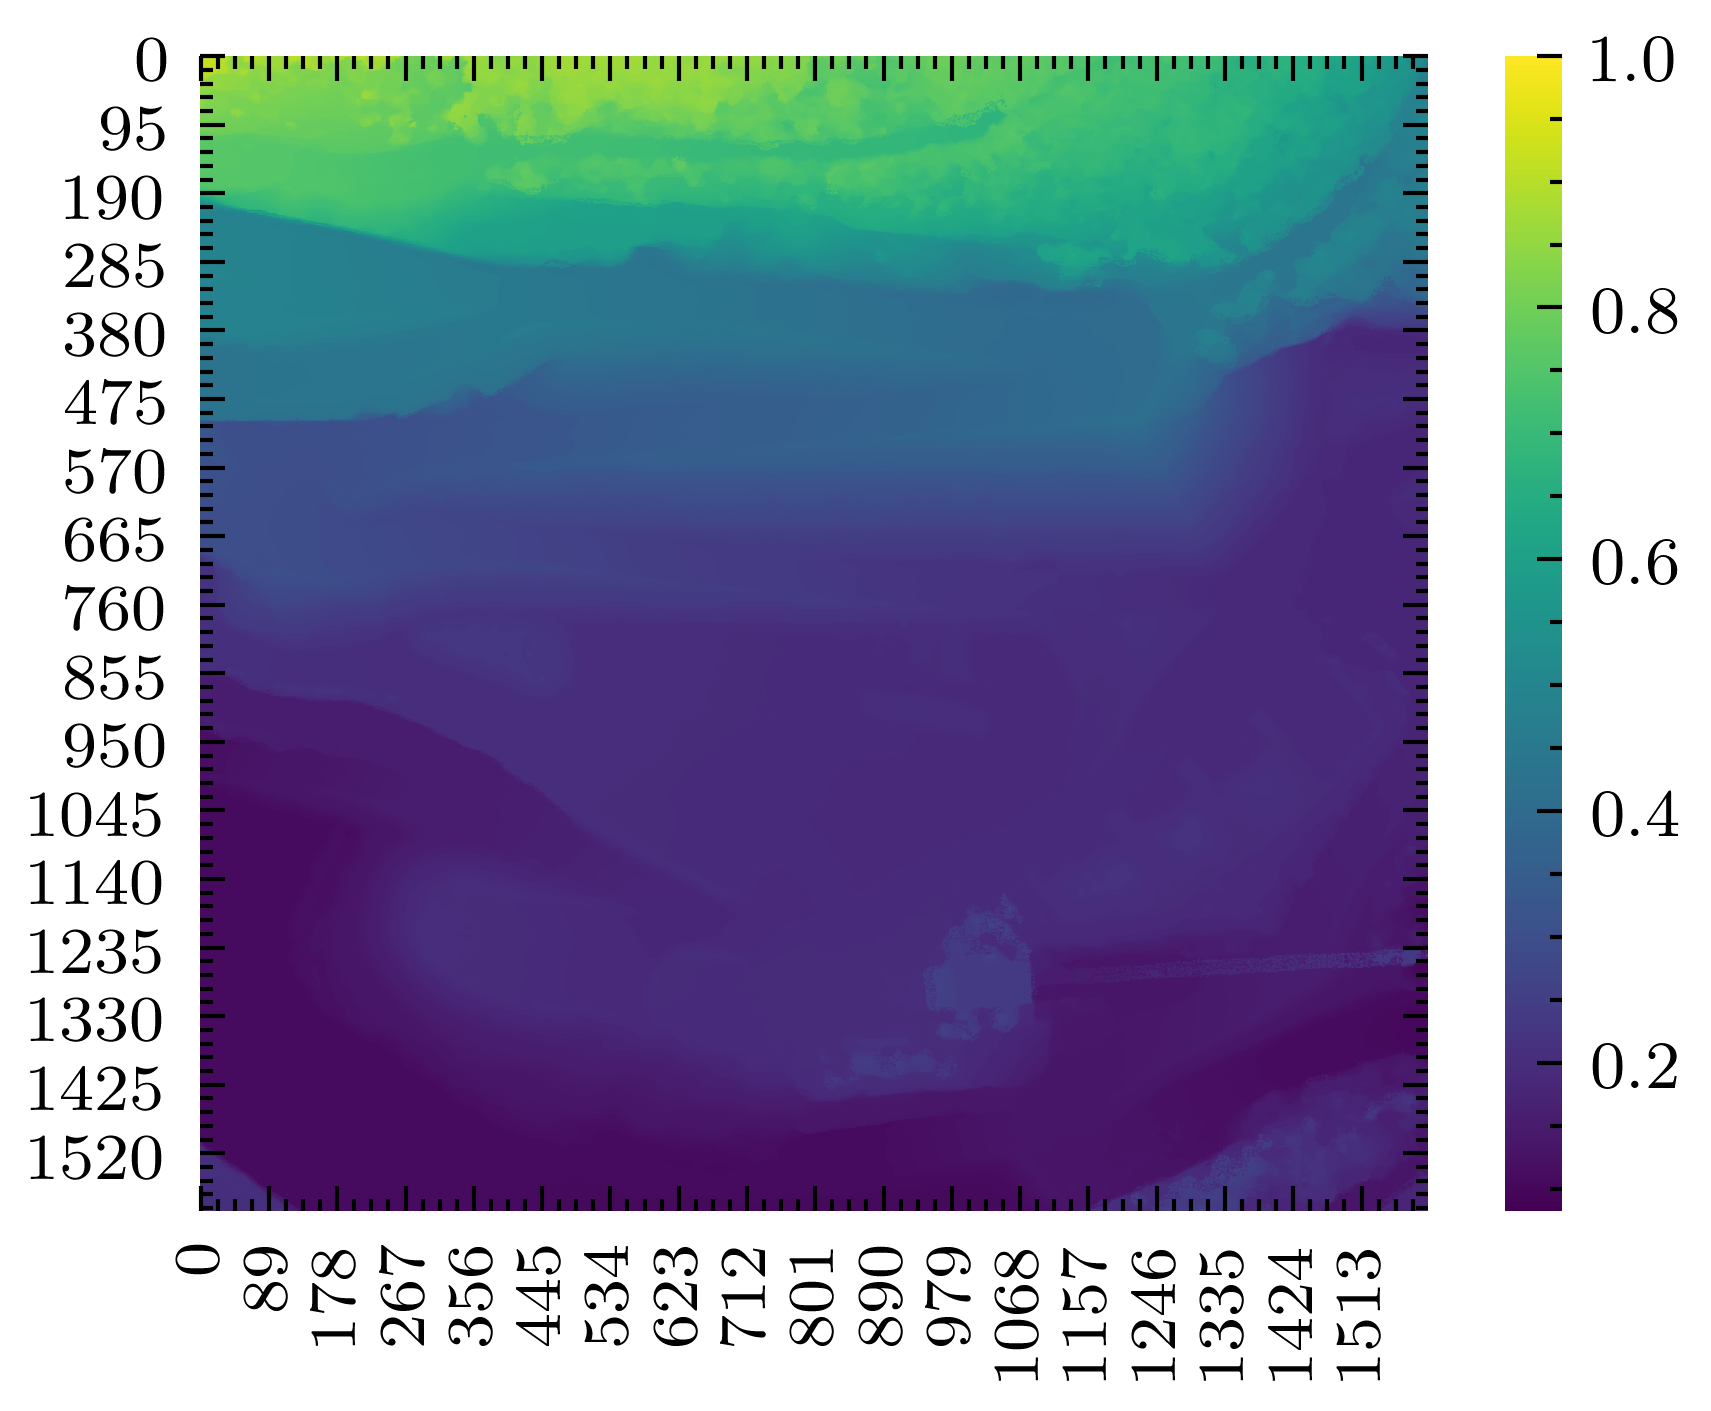
\includegraphics[width=\textwidth]{../img/hm/querry-big-10.png}
            \caption{\emph{Quarry} heightmap}
        \end{subfigure}
        \begin{subfigure}[b]{0.45\linewidth}
            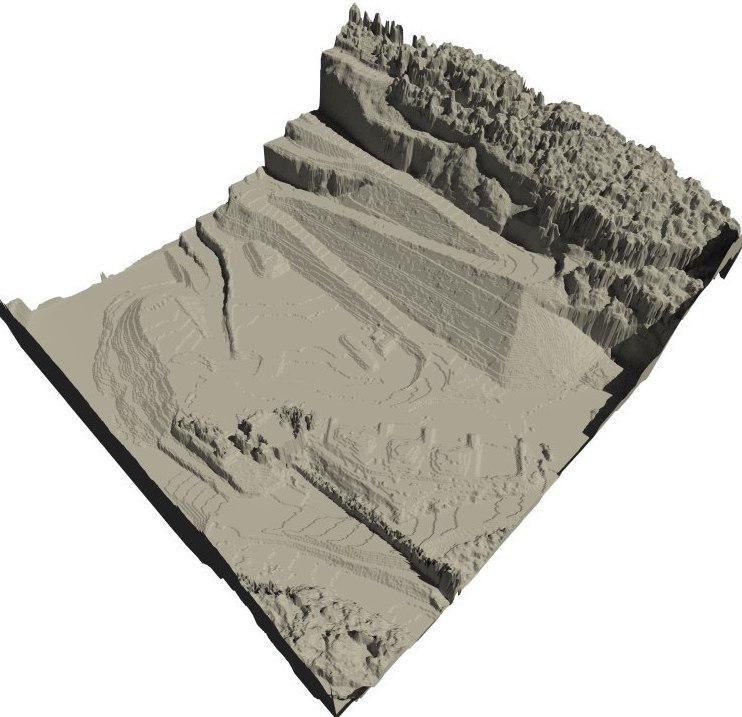
\includegraphics[width=\textwidth]{../img/quarry-rendered.png}
            \caption{\emph{Quarry} map}
            \end{subfigure}    
    \caption{A heightmap}
    \end{figure}
We used thirty maps of $513\times513$ pixel with a resolution of $0.02cm/pixel$ in order to represent a $10\times10m$ region. We generated them by 2D simplex noise \cite{simplex}, a variant of Perlin noise \cite{perlin}, a widely used technique in terrain generation litterature. We created four main categories of terrains: $bumps$, $rails$, $steps$ and $slopes$/$ramps$. For each map we add three different rocky texture to create even more different situations.

\paragraph{Bumps:}
We genered four different maps with increasing bumps using simplex noise with features size $\in[200,100,50,25 ]$. 
\begin{figure}[H]
    \centering
        \begin{subfigure}[b]{0.45\textwidth}
            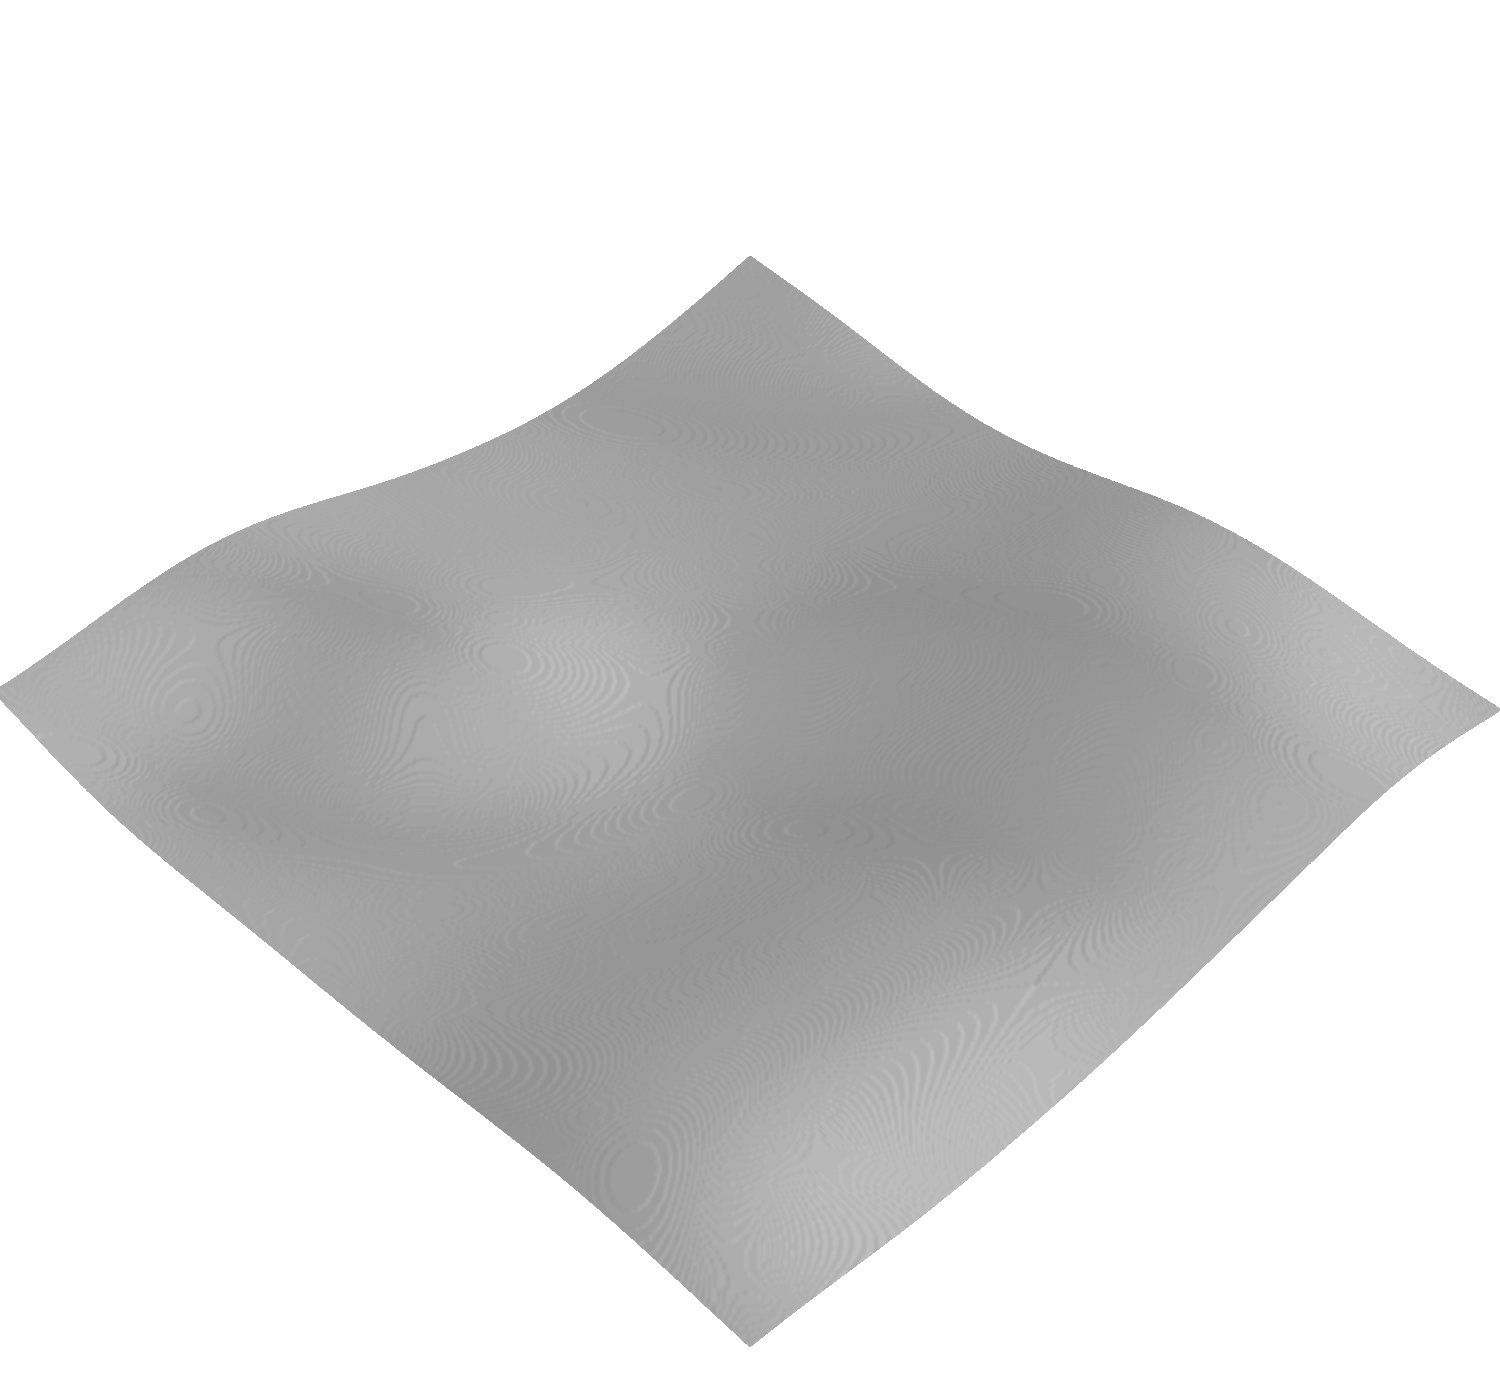
\includegraphics[width=\textwidth]{../img/hm3d/bumps0.png}
            \caption{\emph{bumps0}}
        \end{subfigure}
        \begin{subfigure}[b]{0.45\linewidth}
            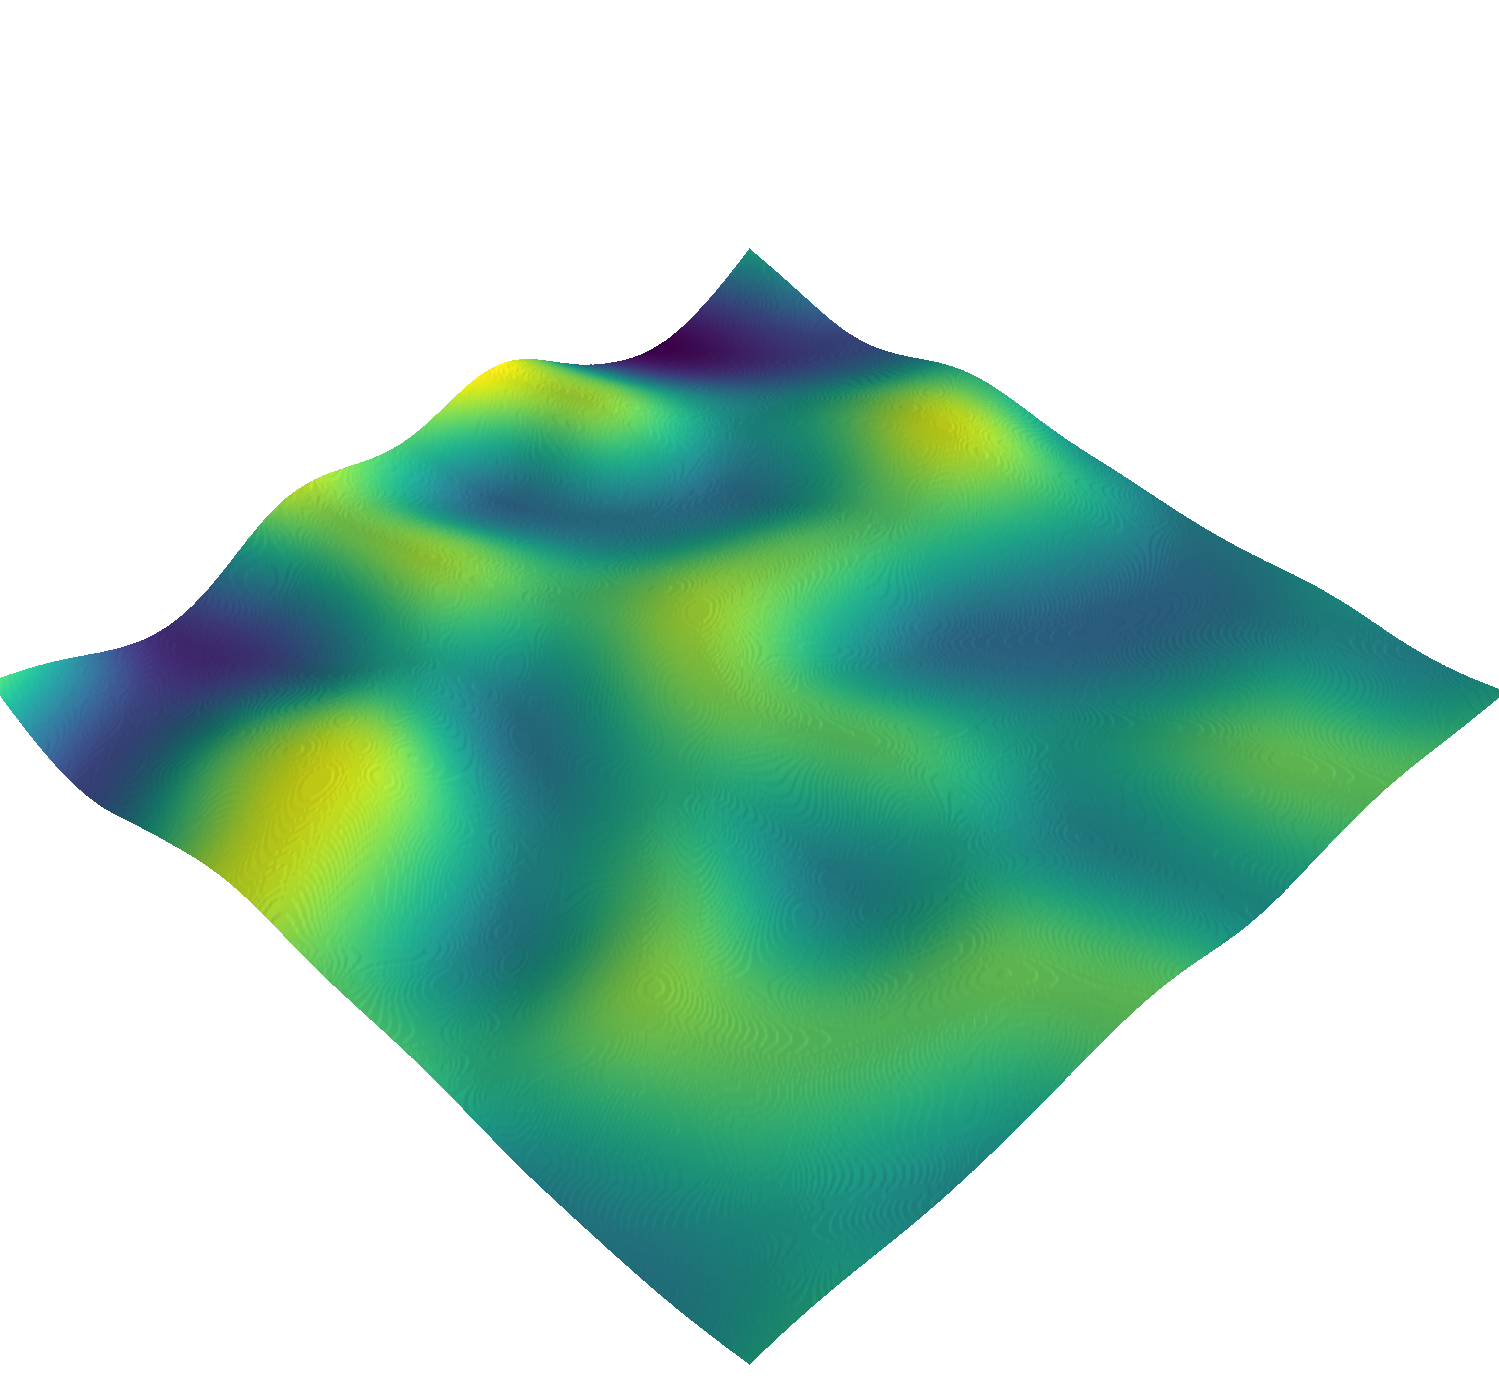
\includegraphics[width=\textwidth]{../img/hm3d/bumps1.png}
            \caption{\emph{bumps1}}
            \end{subfigure}    
          \begin{subfigure}[b]{0.45\textwidth}
            
\includegraphics[width=\textwidth]{../img/hm3d/bumps2.png}
            \caption{\emph{bumps2}}
        \end{subfigure}    
        \begin{subfigure}[b]{0.45\textwidth}
            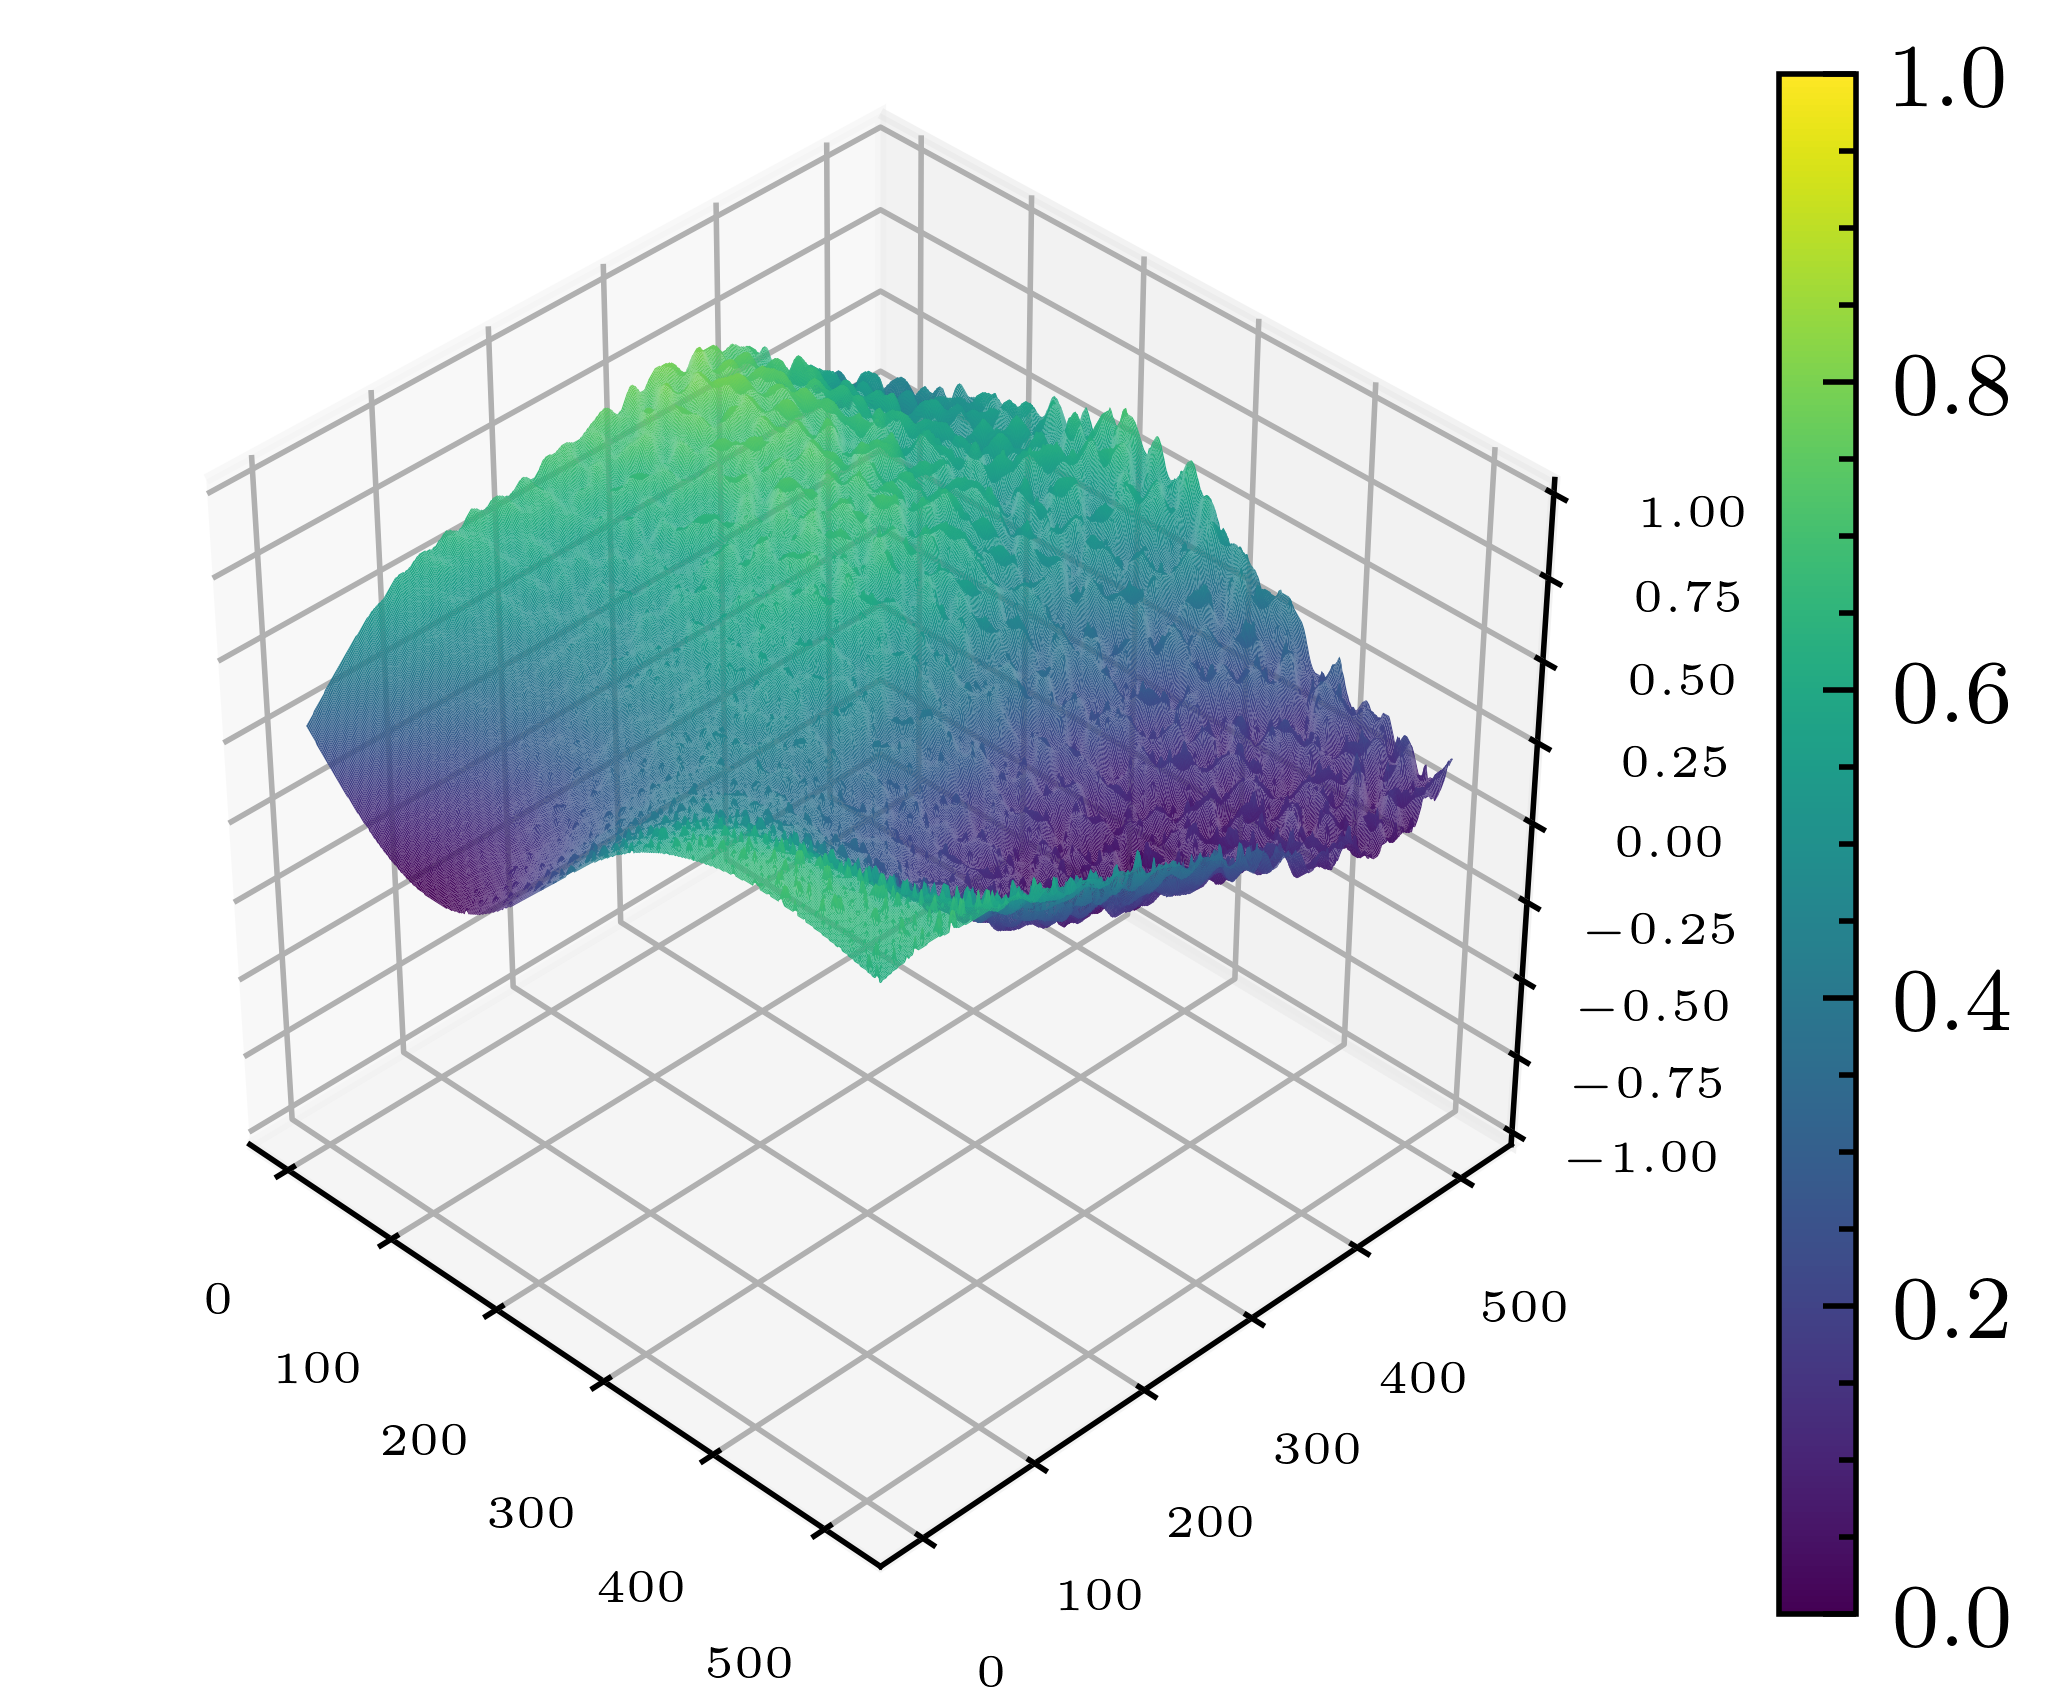
\includegraphics[width=\textwidth]{../img/hm3d/bumps3.png}
            \caption{\emph{bumps3}}
        \end{subfigure}    
    \label{fig: heightmaps}
    \caption{Bumps maps.}
\end{figure}
\paragraph{Bars:} in these maps there are wall with different shapes and heights. In 
\begin{figure}[H]
    \centering
        \begin{subfigure}[b]{0.45\textwidth}
            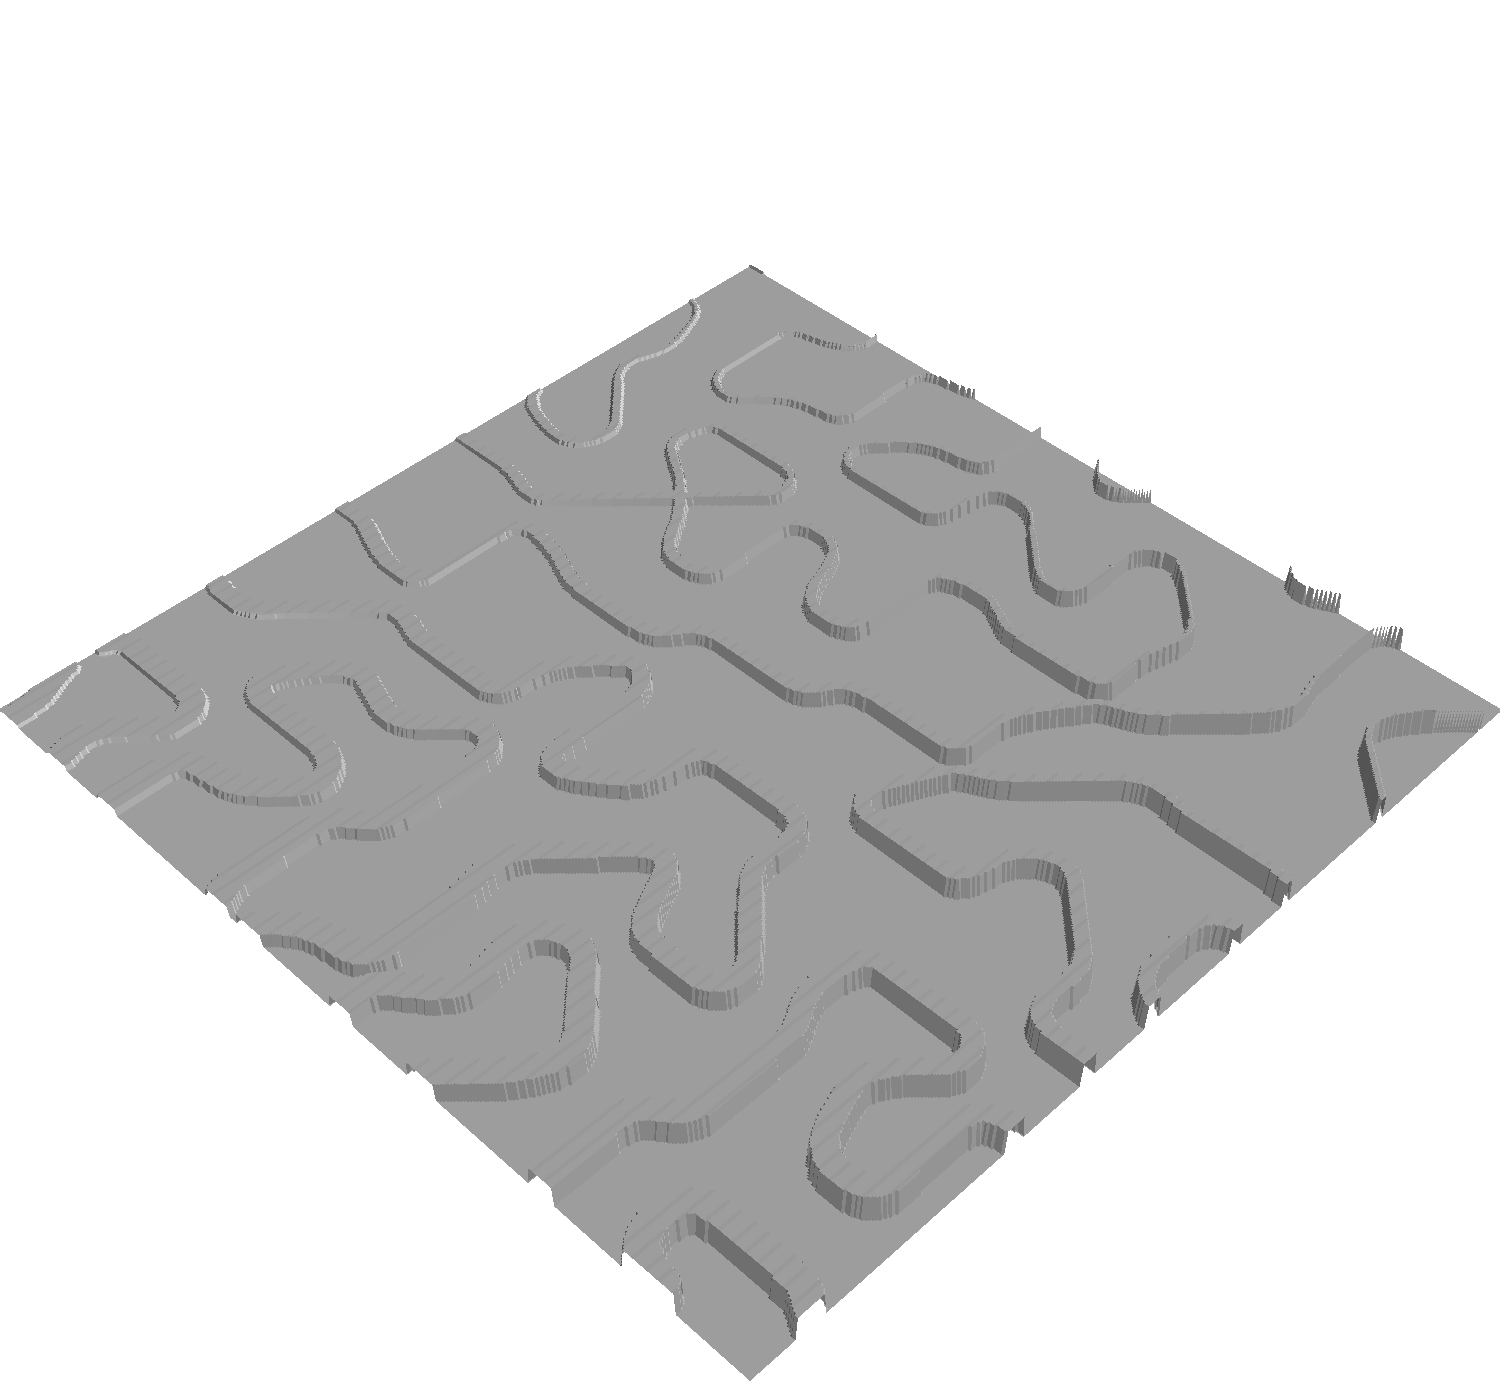
\includegraphics[width=\textwidth]{../img/hm3d/bars1.png}
            \caption{\emph{bars1}}
        \end{subfigure}
        \begin{subfigure}[b]{0.45\linewidth}
            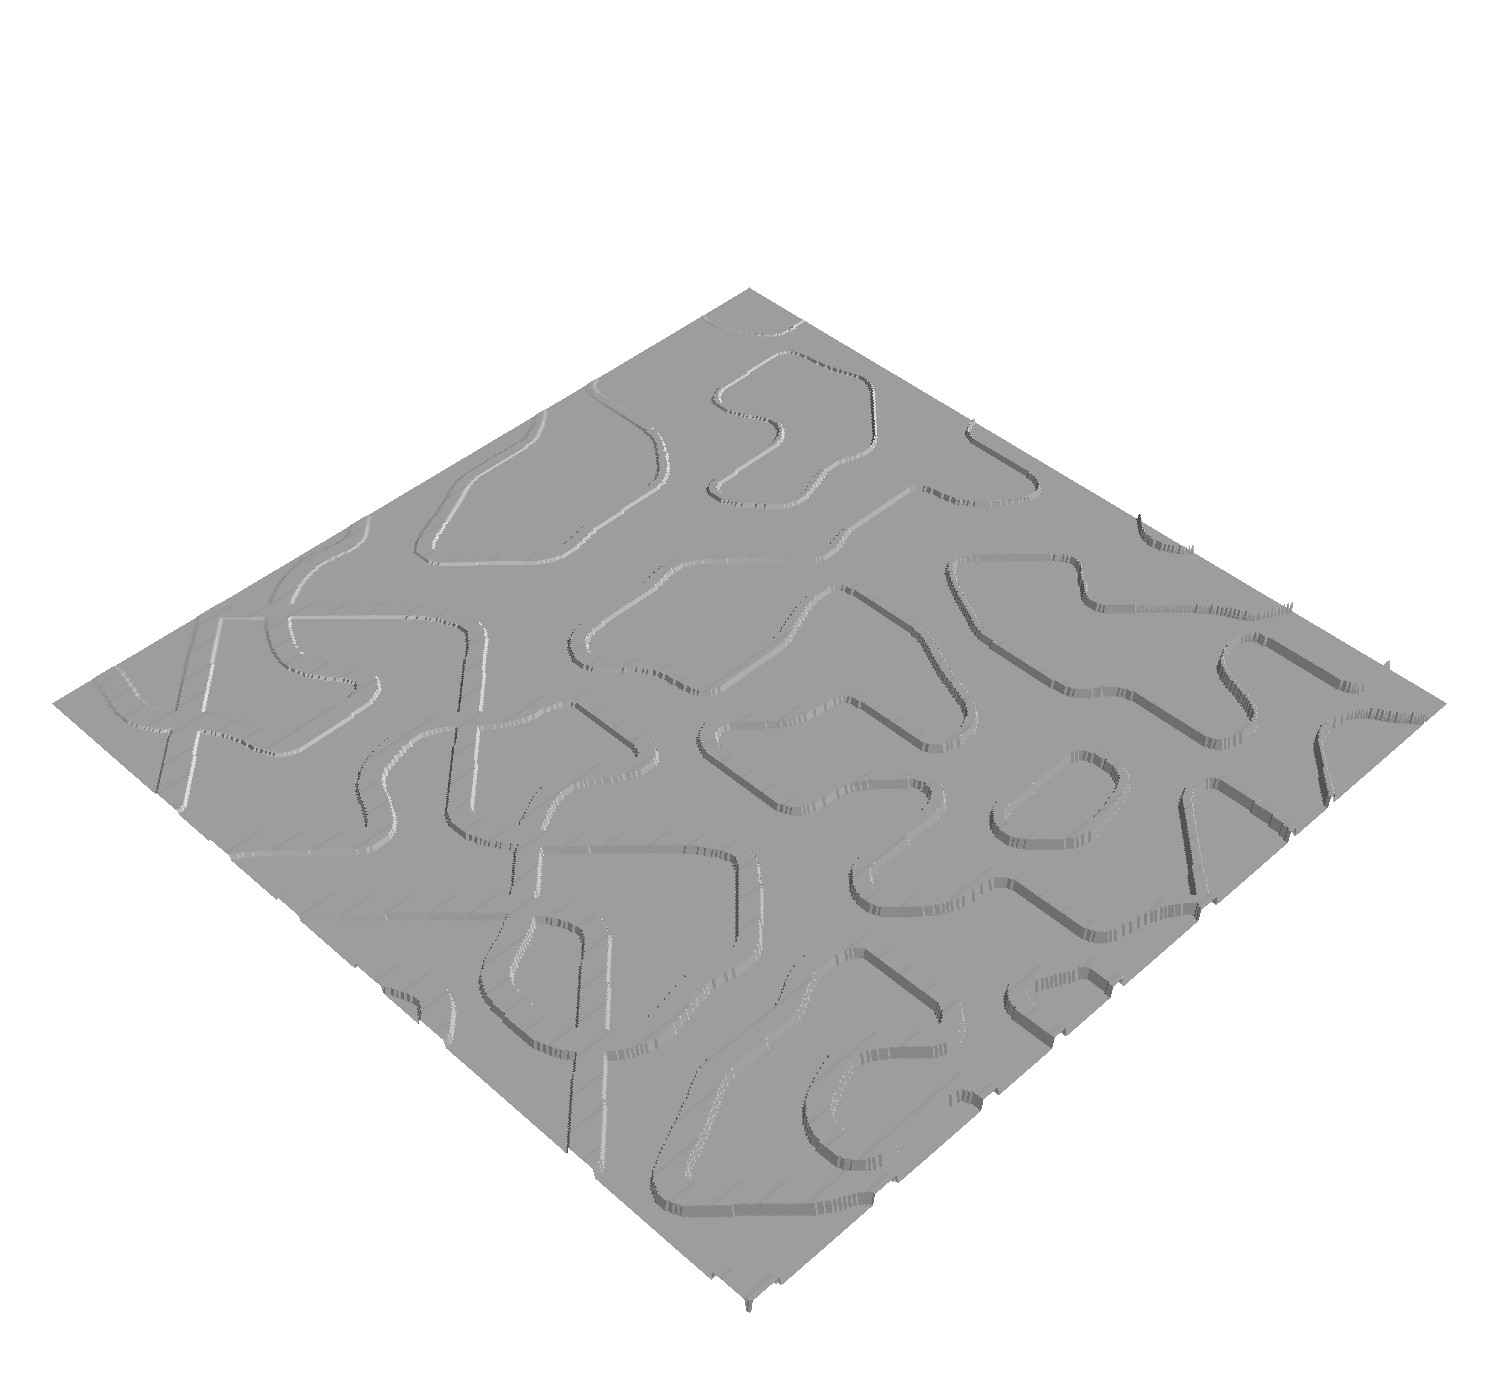
\includegraphics[width=\textwidth]{../img/hm3d/bars3.png}
            \caption{\emph{bars3}}
            \end{subfigure}     
    \label{fig: heightmaps}
    \caption{Bars maps.}
\end{figure}
\paragraph{Rails:} ground with slots.
\begin{figure}[H]
    \centering
        \begin{subfigure}[b]{0.45\textwidth}
            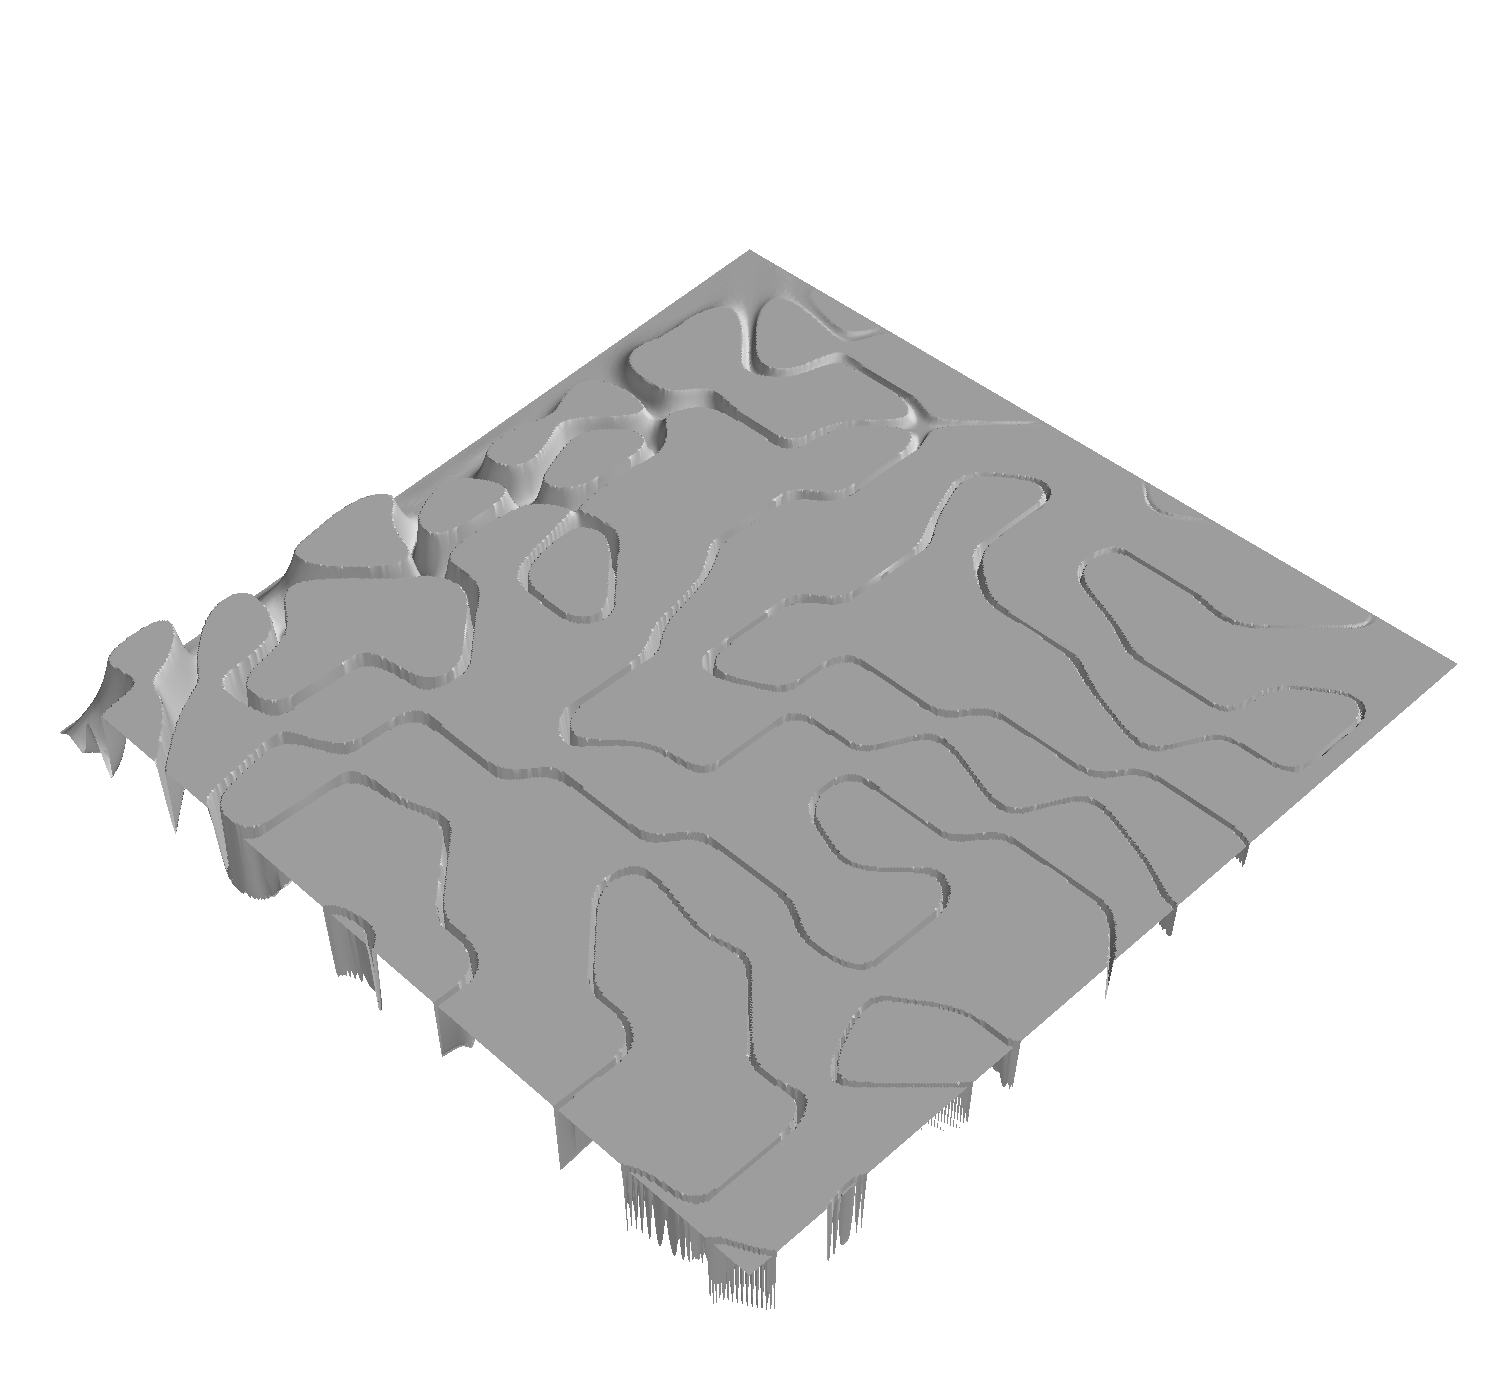
\includegraphics[width=\textwidth]{../img/hm3d/rails1.png}
            \caption{\emph{rails1}}
        \end{subfigure}
        \begin{subfigure}[b]{0.45\linewidth}
            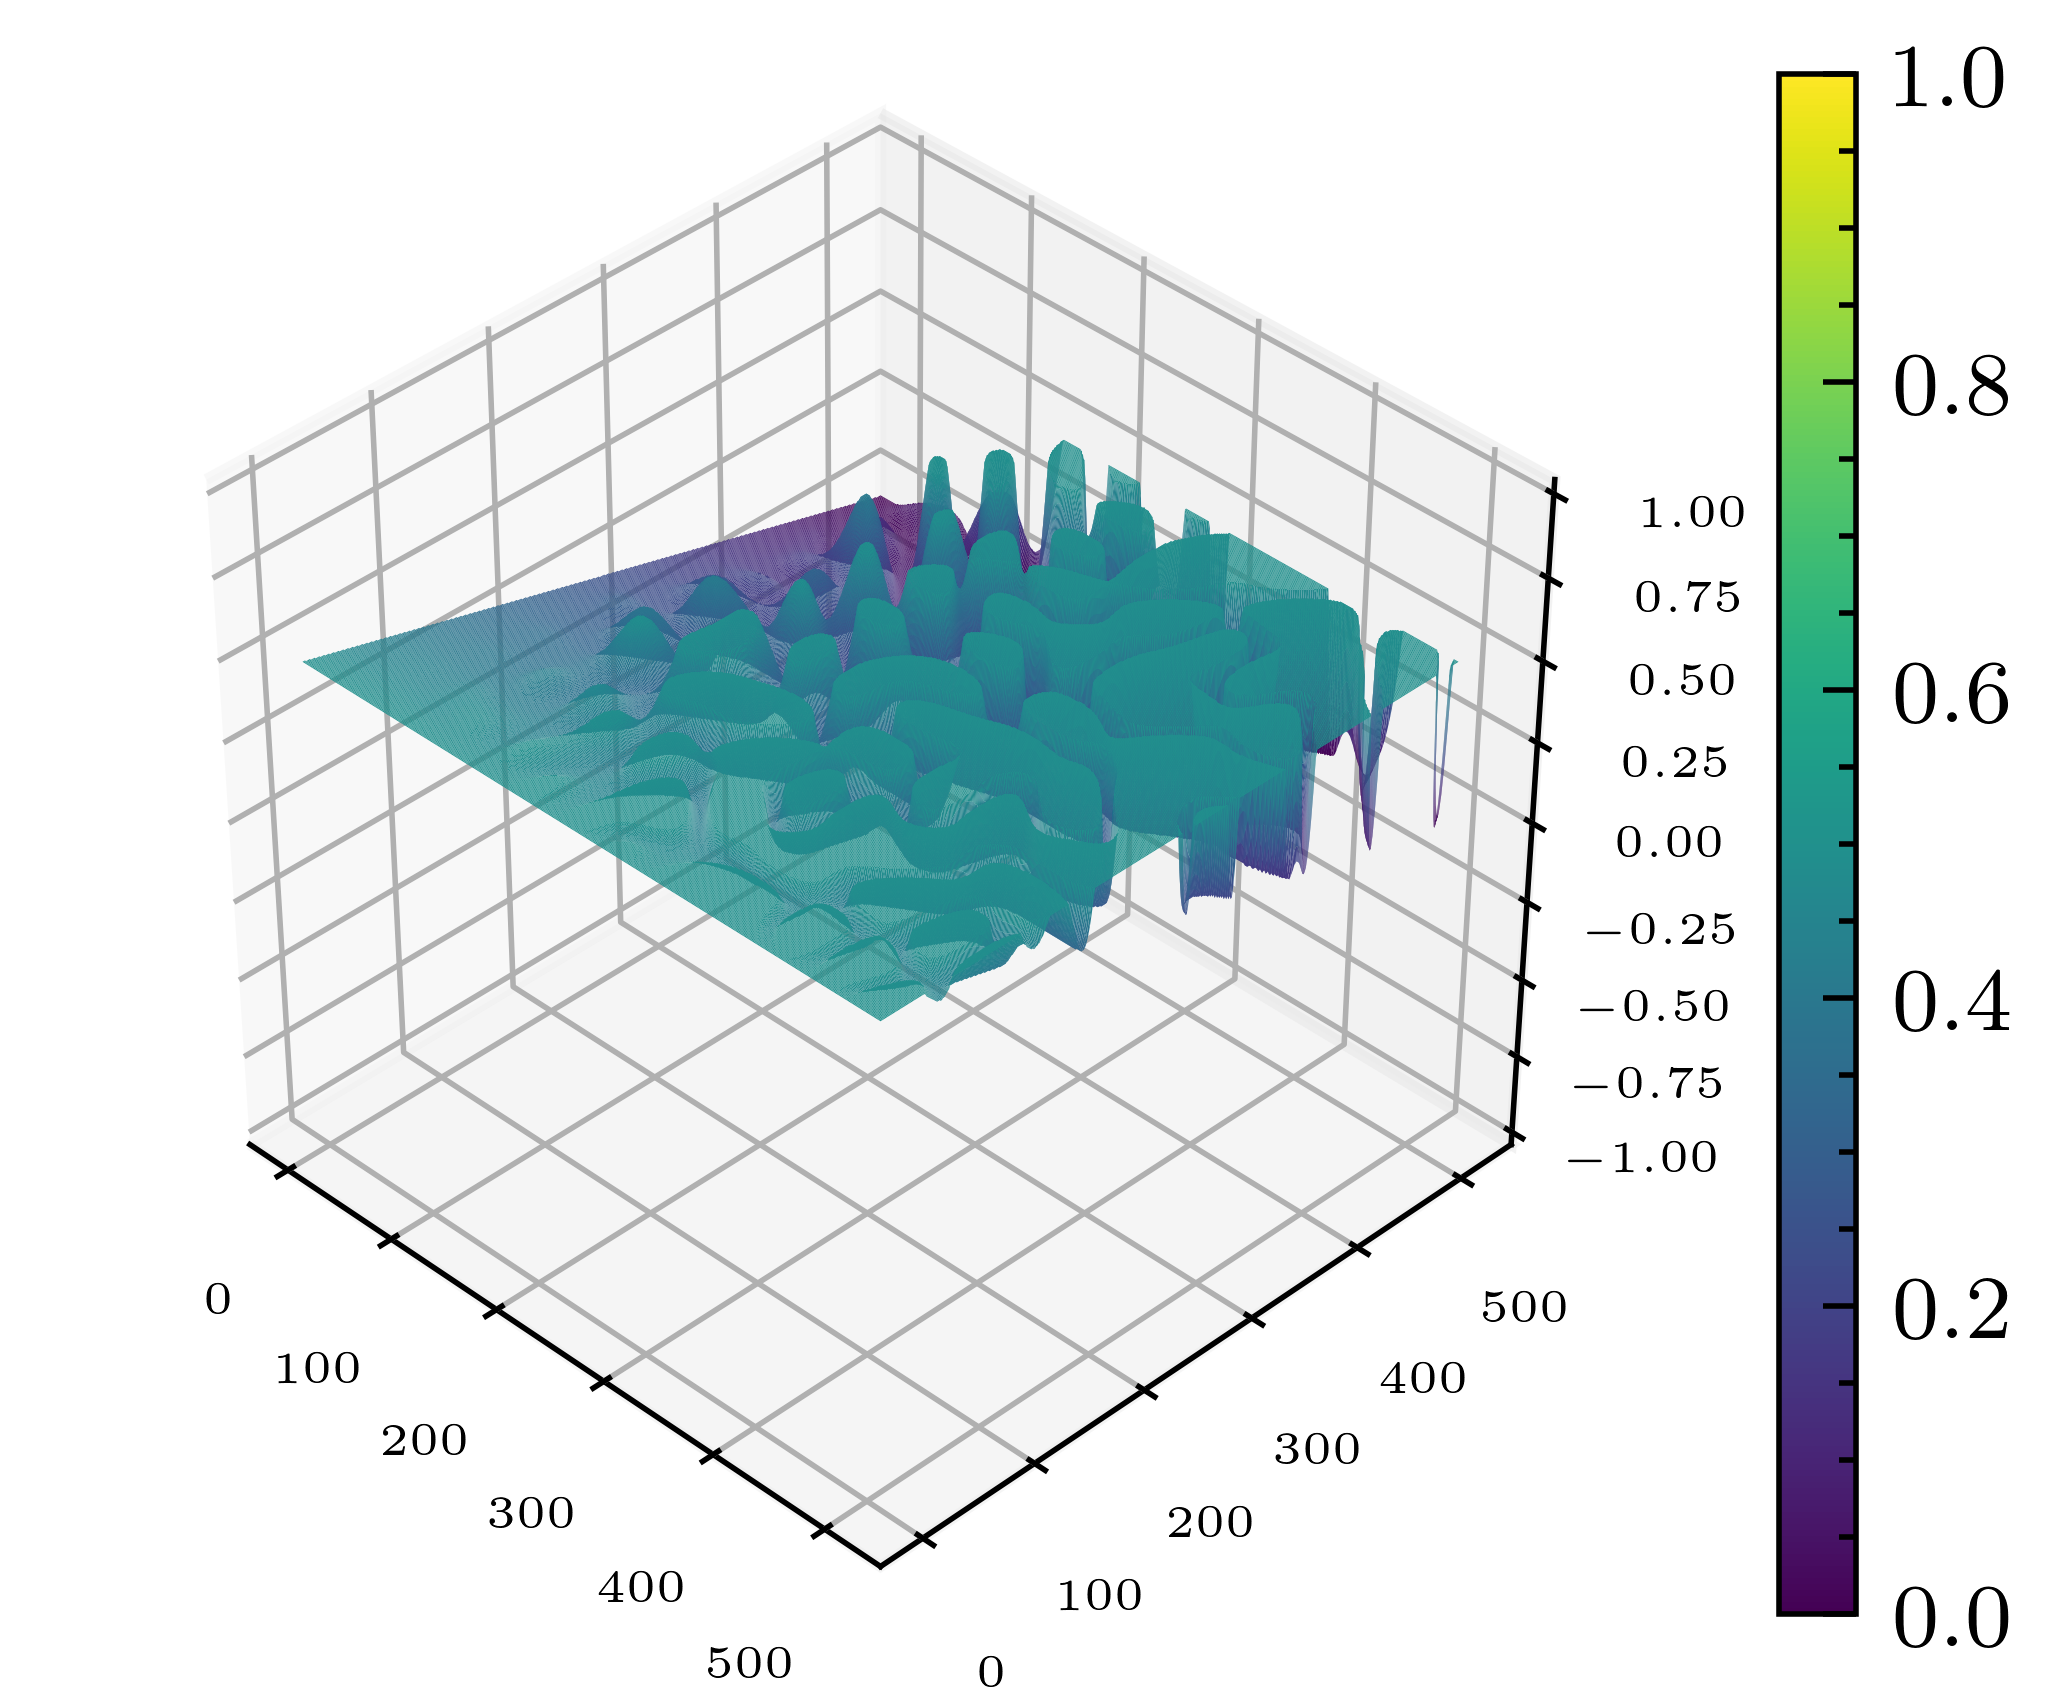
\includegraphics[width=\textwidth]{../img/hm3d/rails2.png}
            \caption{\emph{rails2}}
            \end{subfigure}    
          \begin{subfigure}[b]{0.45\textwidth}
            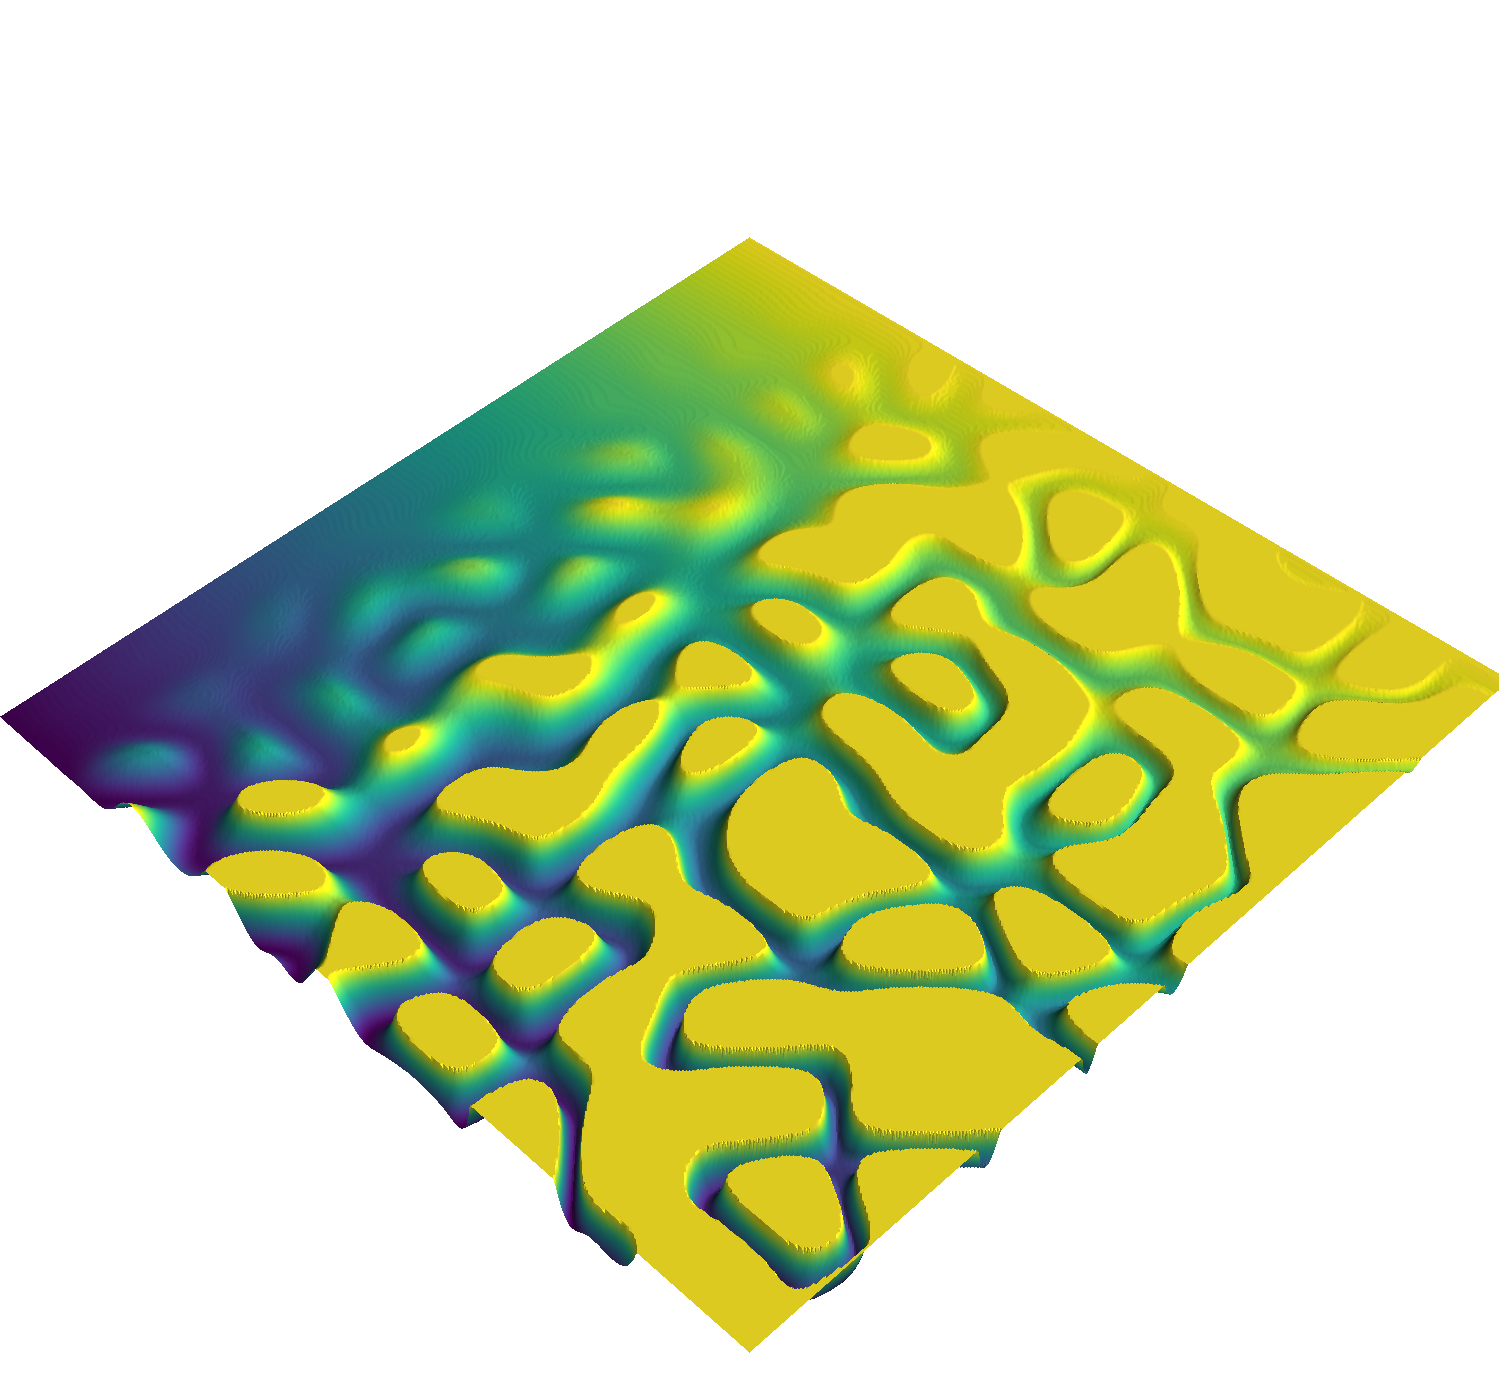
\includegraphics[width=\textwidth]{../img/hm3d/rails3.png}
            \caption{\emph{rails3}}
        \end{subfigure}    
    \label{fig: heightmaps}
    \caption{Rails maps.}
\end{figure}
\paragraph{Steps:} There are maps have huge wall and holes
\begin{figure}[H]
    \centering
        \begin{subfigure}[b]{0.45\textwidth}
            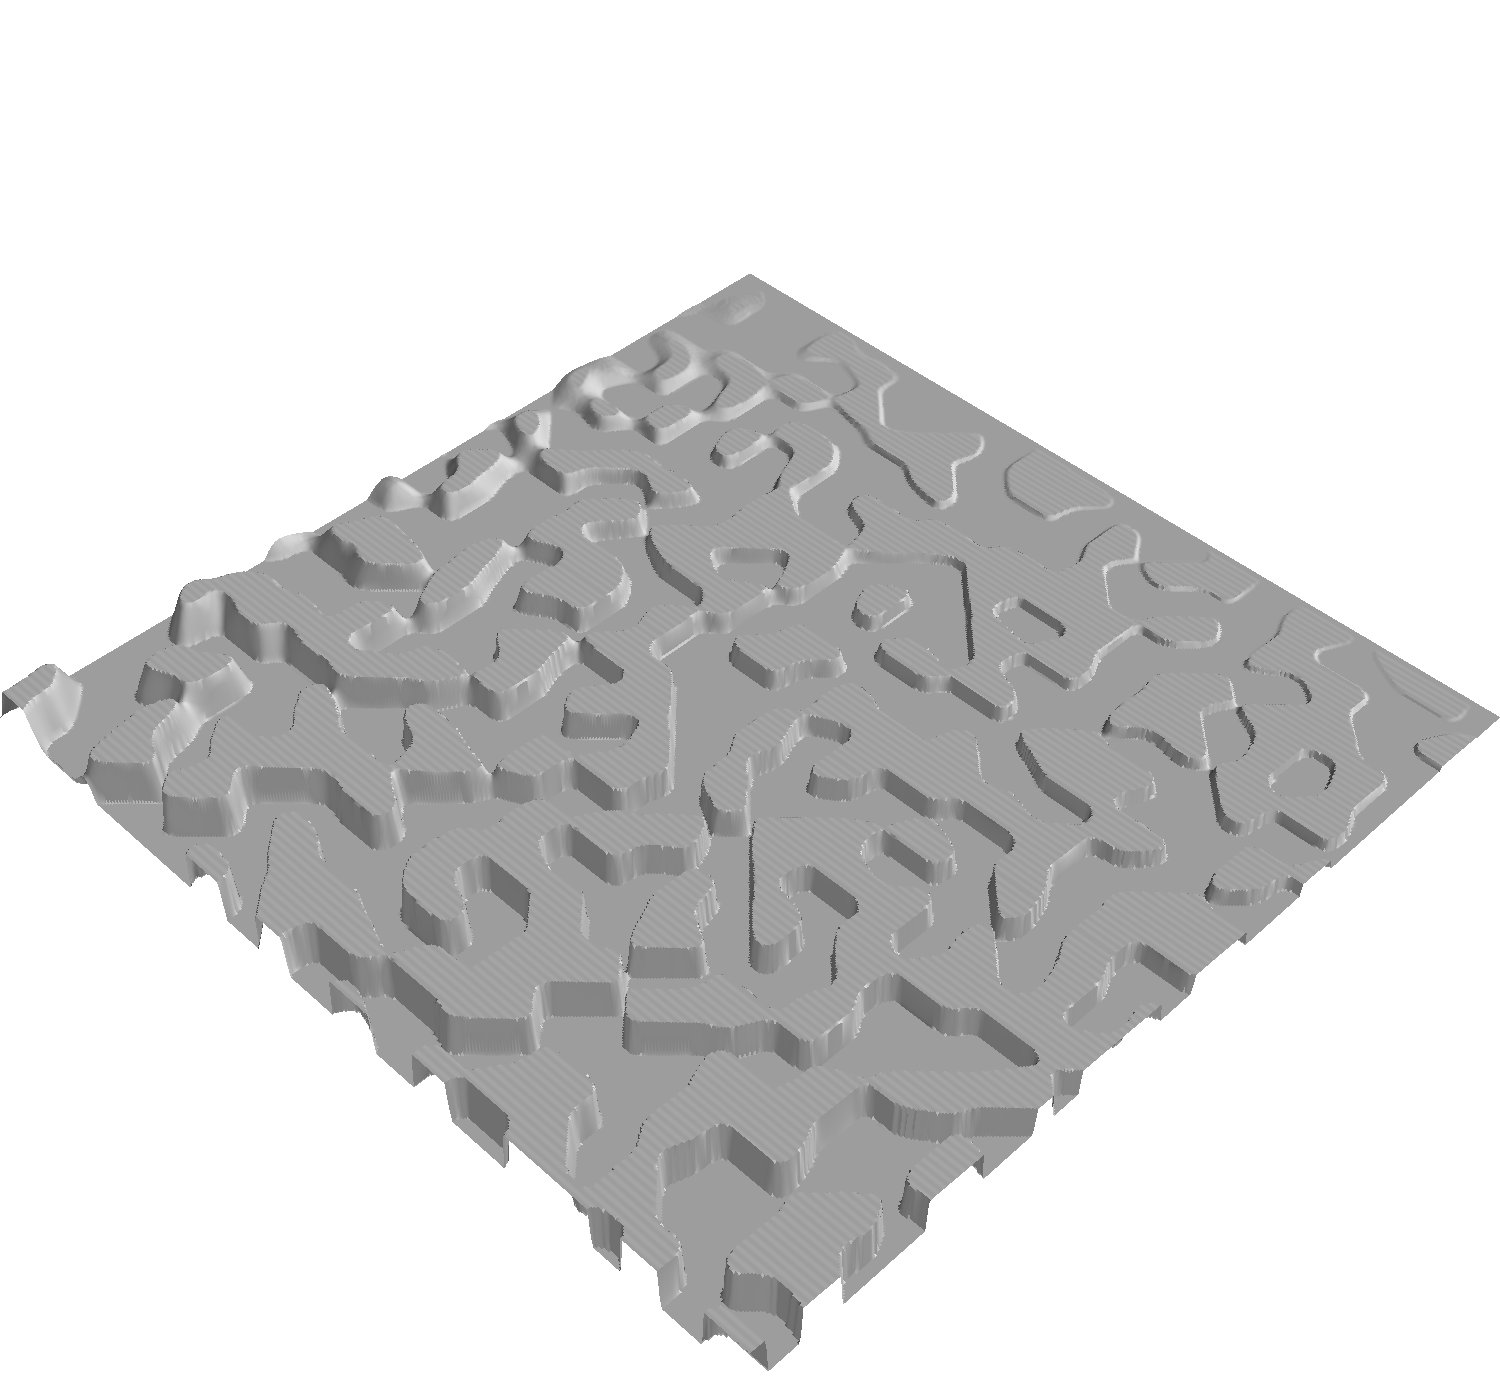
\includegraphics[width=\textwidth]{../img/hm3d/steps1.png}
            \caption{\emph{steps1}}
        \end{subfigure}
        \begin{subfigure}[b]{0.45\linewidth}
            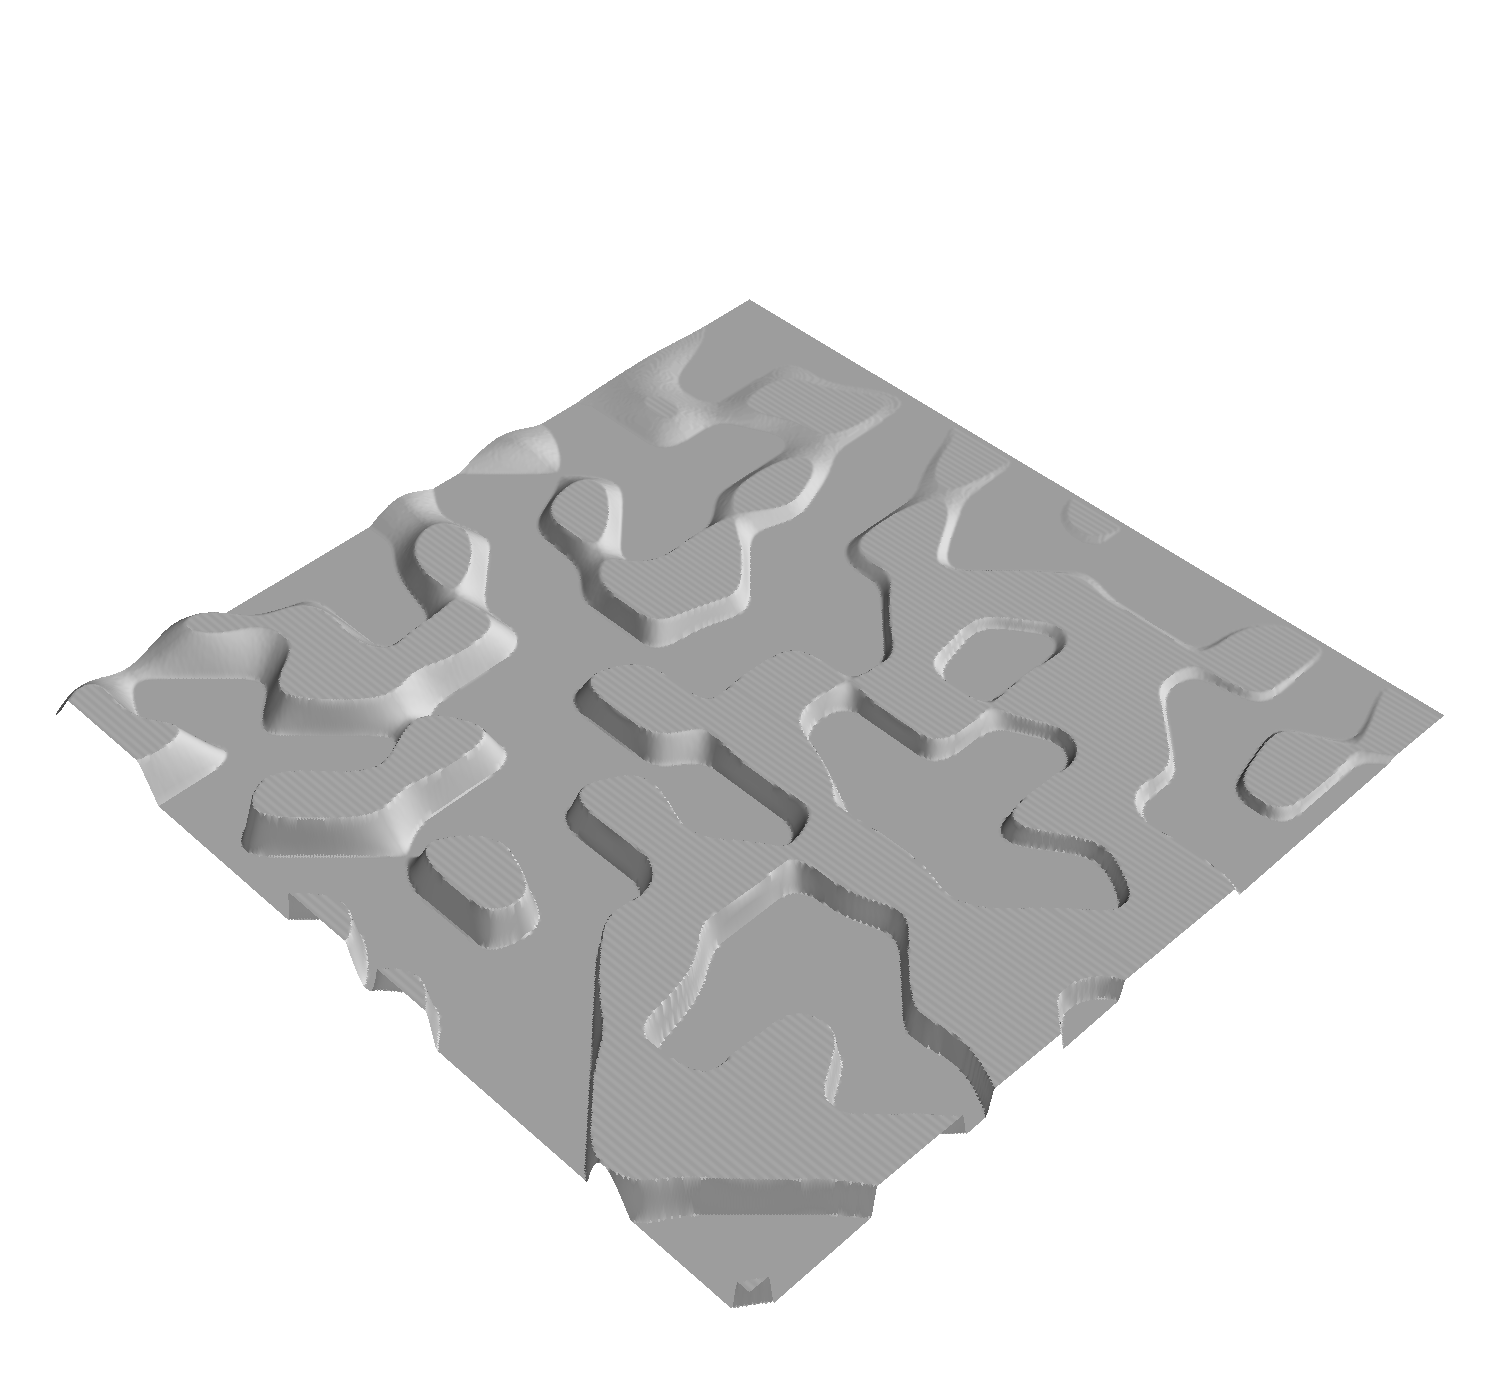
\includegraphics[width=\textwidth]{../img/hm3d/steps2.png}
            \caption{\emph{steps2}}
            \end{subfigure}    
          \begin{subfigure}[b]{0.45\textwidth}
            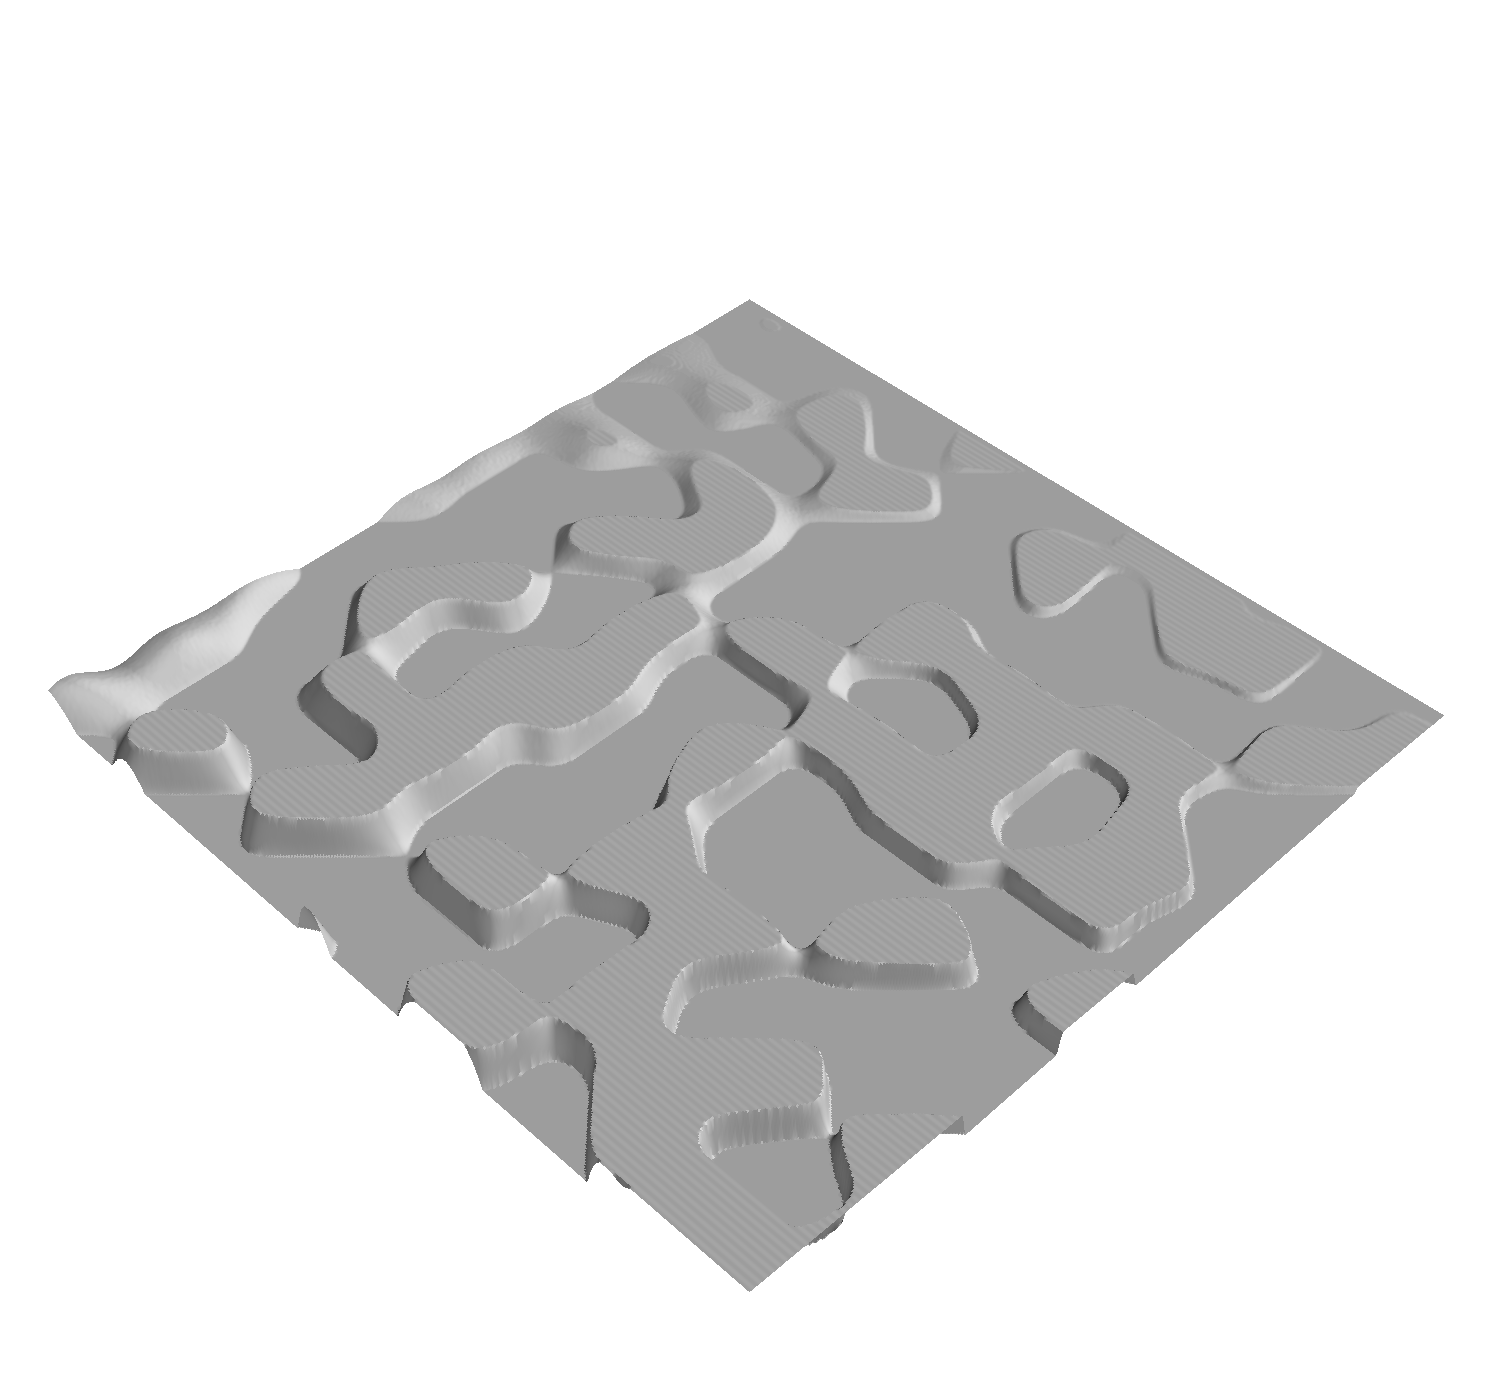
\includegraphics[width=\textwidth]{../img/hm3d/steps3.png}
            \caption{\emph{steps3}}
        \end{subfigure}    
    \label{fig: heightmaps}
    \caption{Steps maps.}
\end{figure}
\paragraph{Slopes/Ramps:} uneven terrain scaled by different height factors from $3$ to $5$ used to include samples where \emph{Krock} has to climb.
\begin{figure}[H]
    \centering
        \begin{subfigure}[b]{0.45\textwidth}
            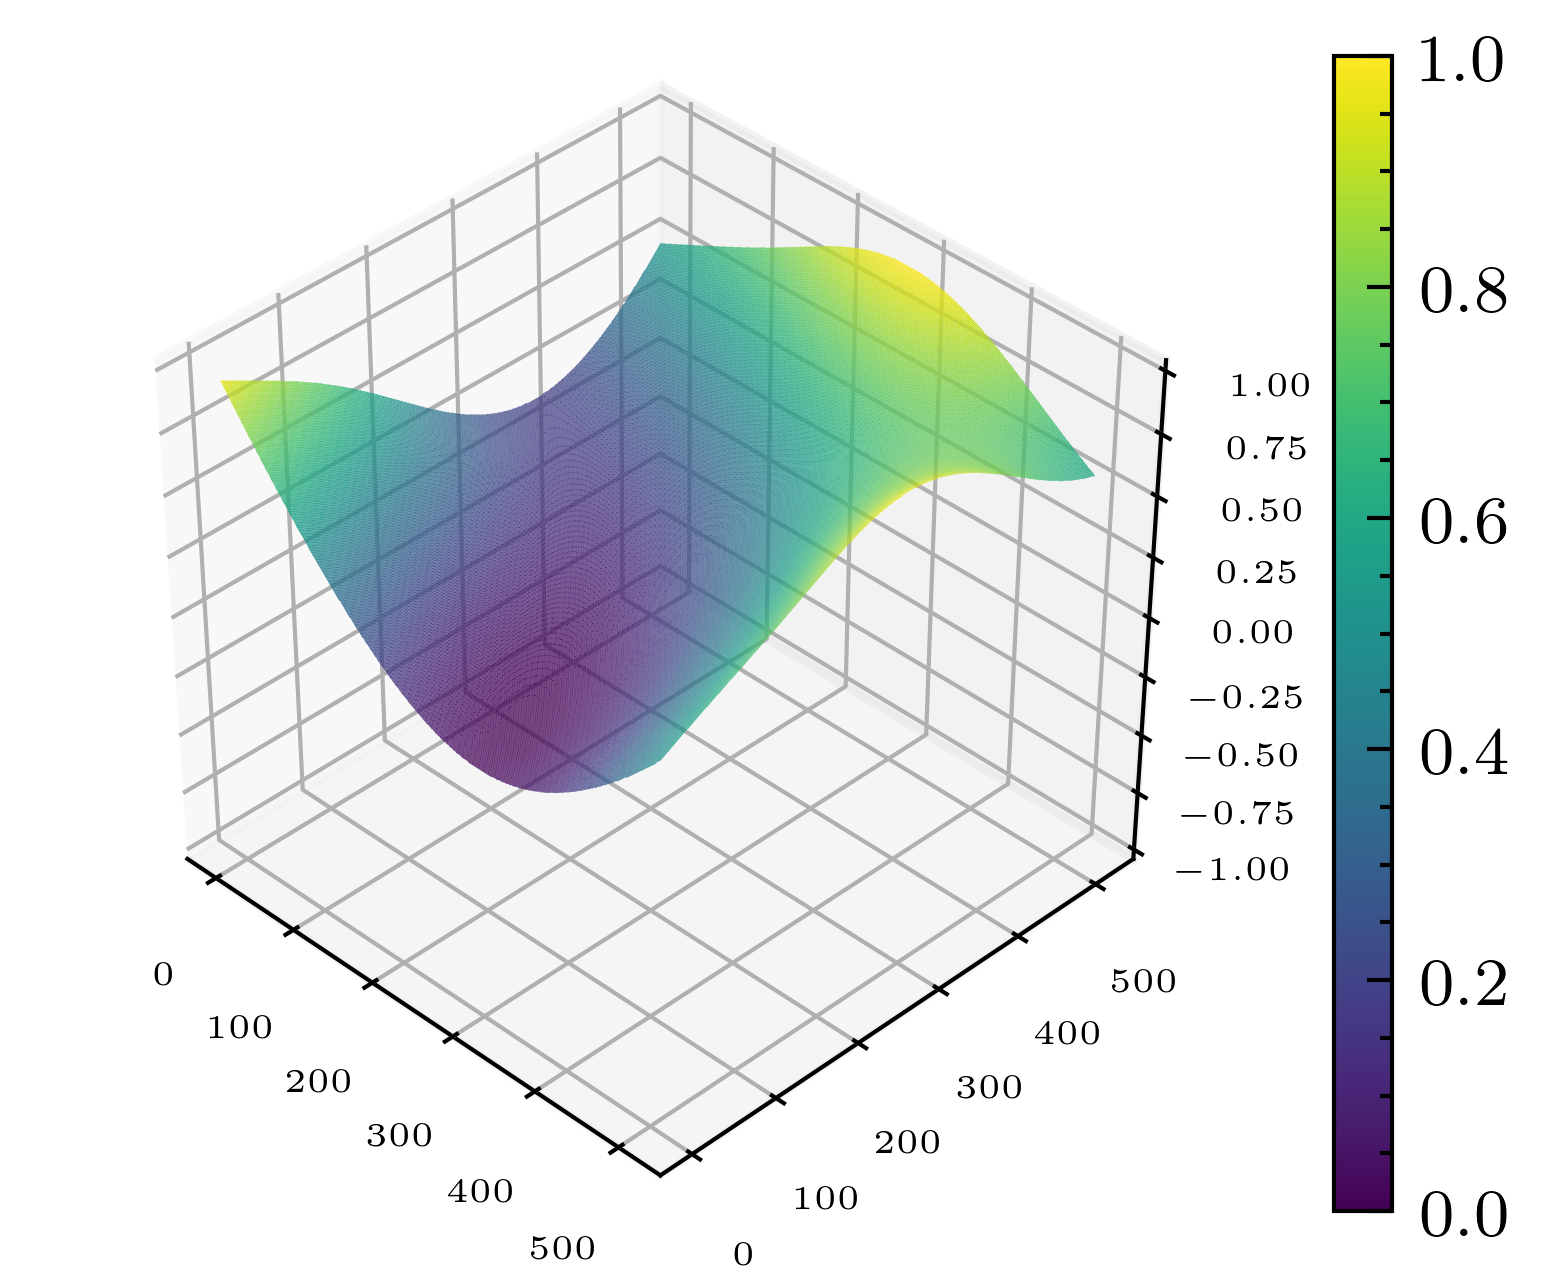
\includegraphics[width=\textwidth]{../img/hm3d/ramp0.png}
            \caption{\emph{ramp0}}
        \end{subfigure}
        \begin{subfigure}[b]{0.45\linewidth}
            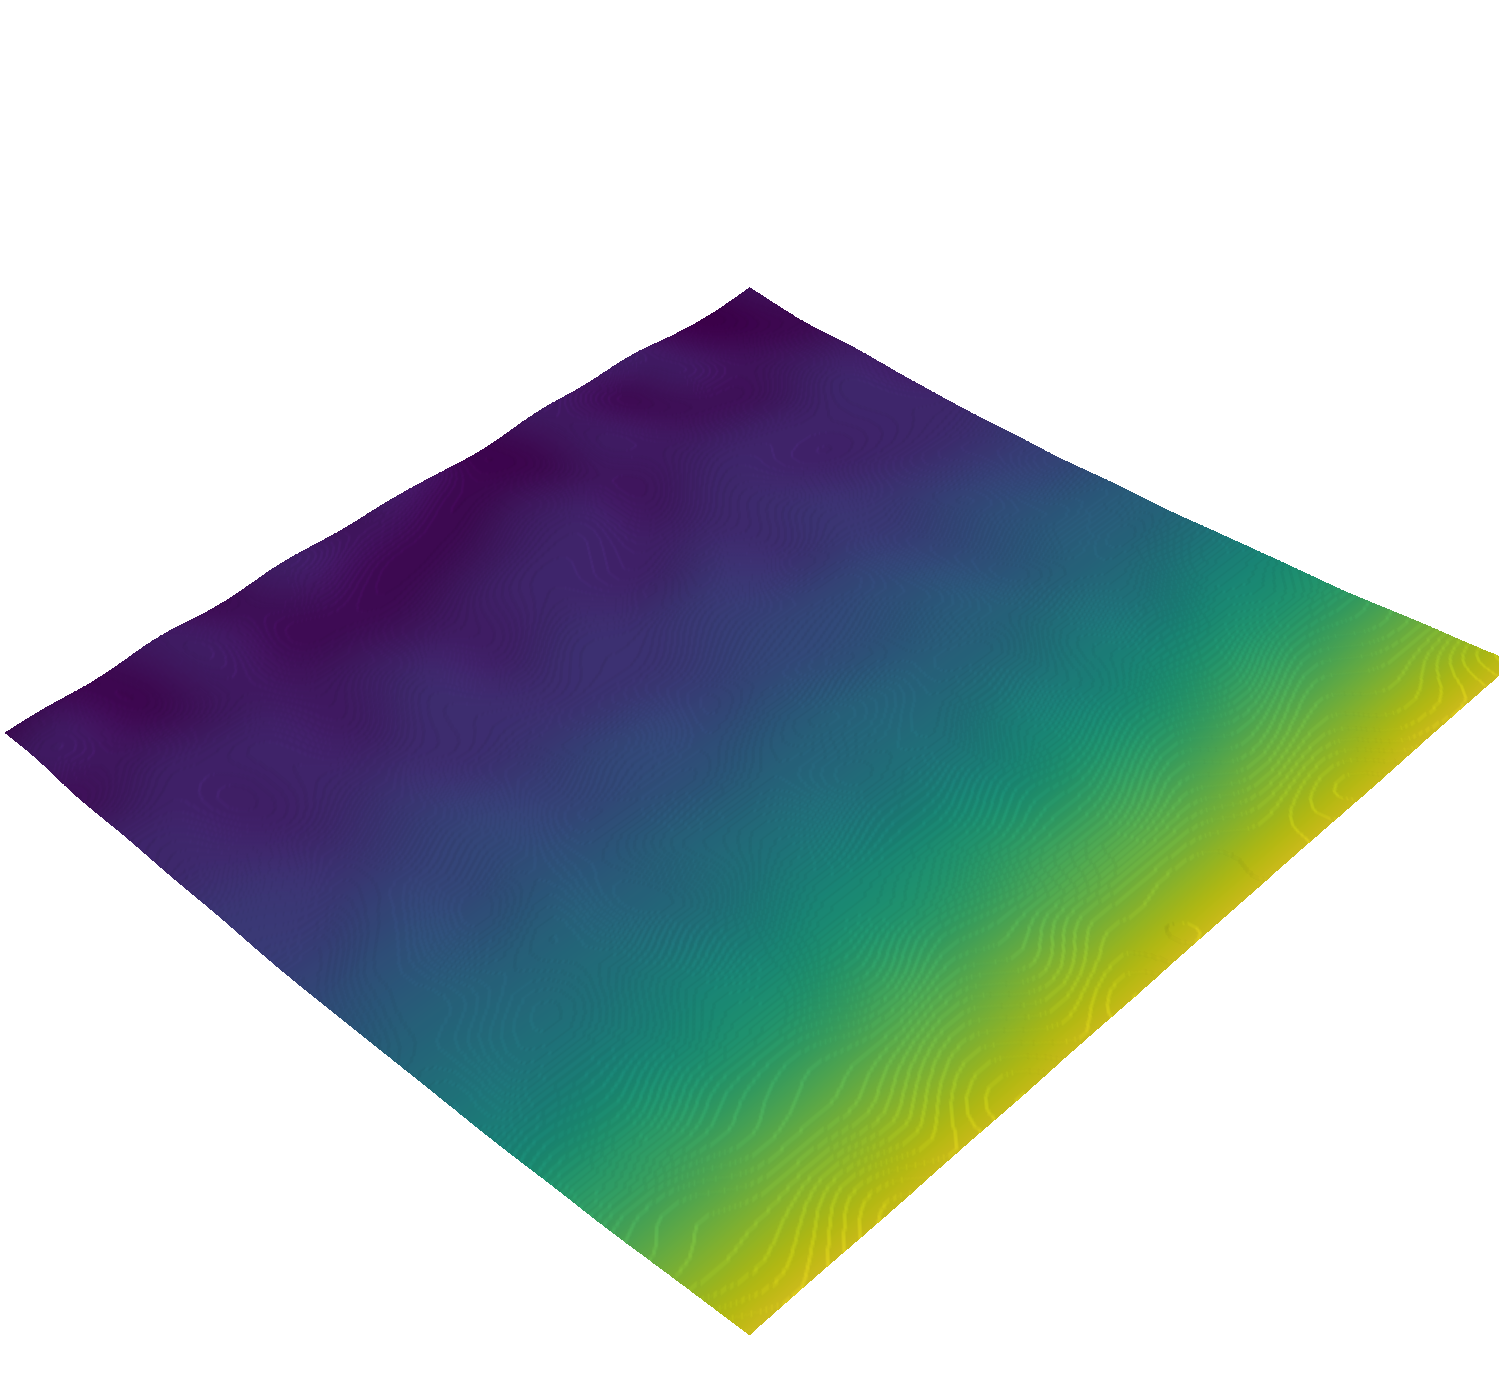
\includegraphics[width=\textwidth]{../img/hm3d/ramp1.png}
            \caption{\emph{ramp1}}
            \end{subfigure}    
          \begin{subfigure}[b]{0.45\textwidth}
            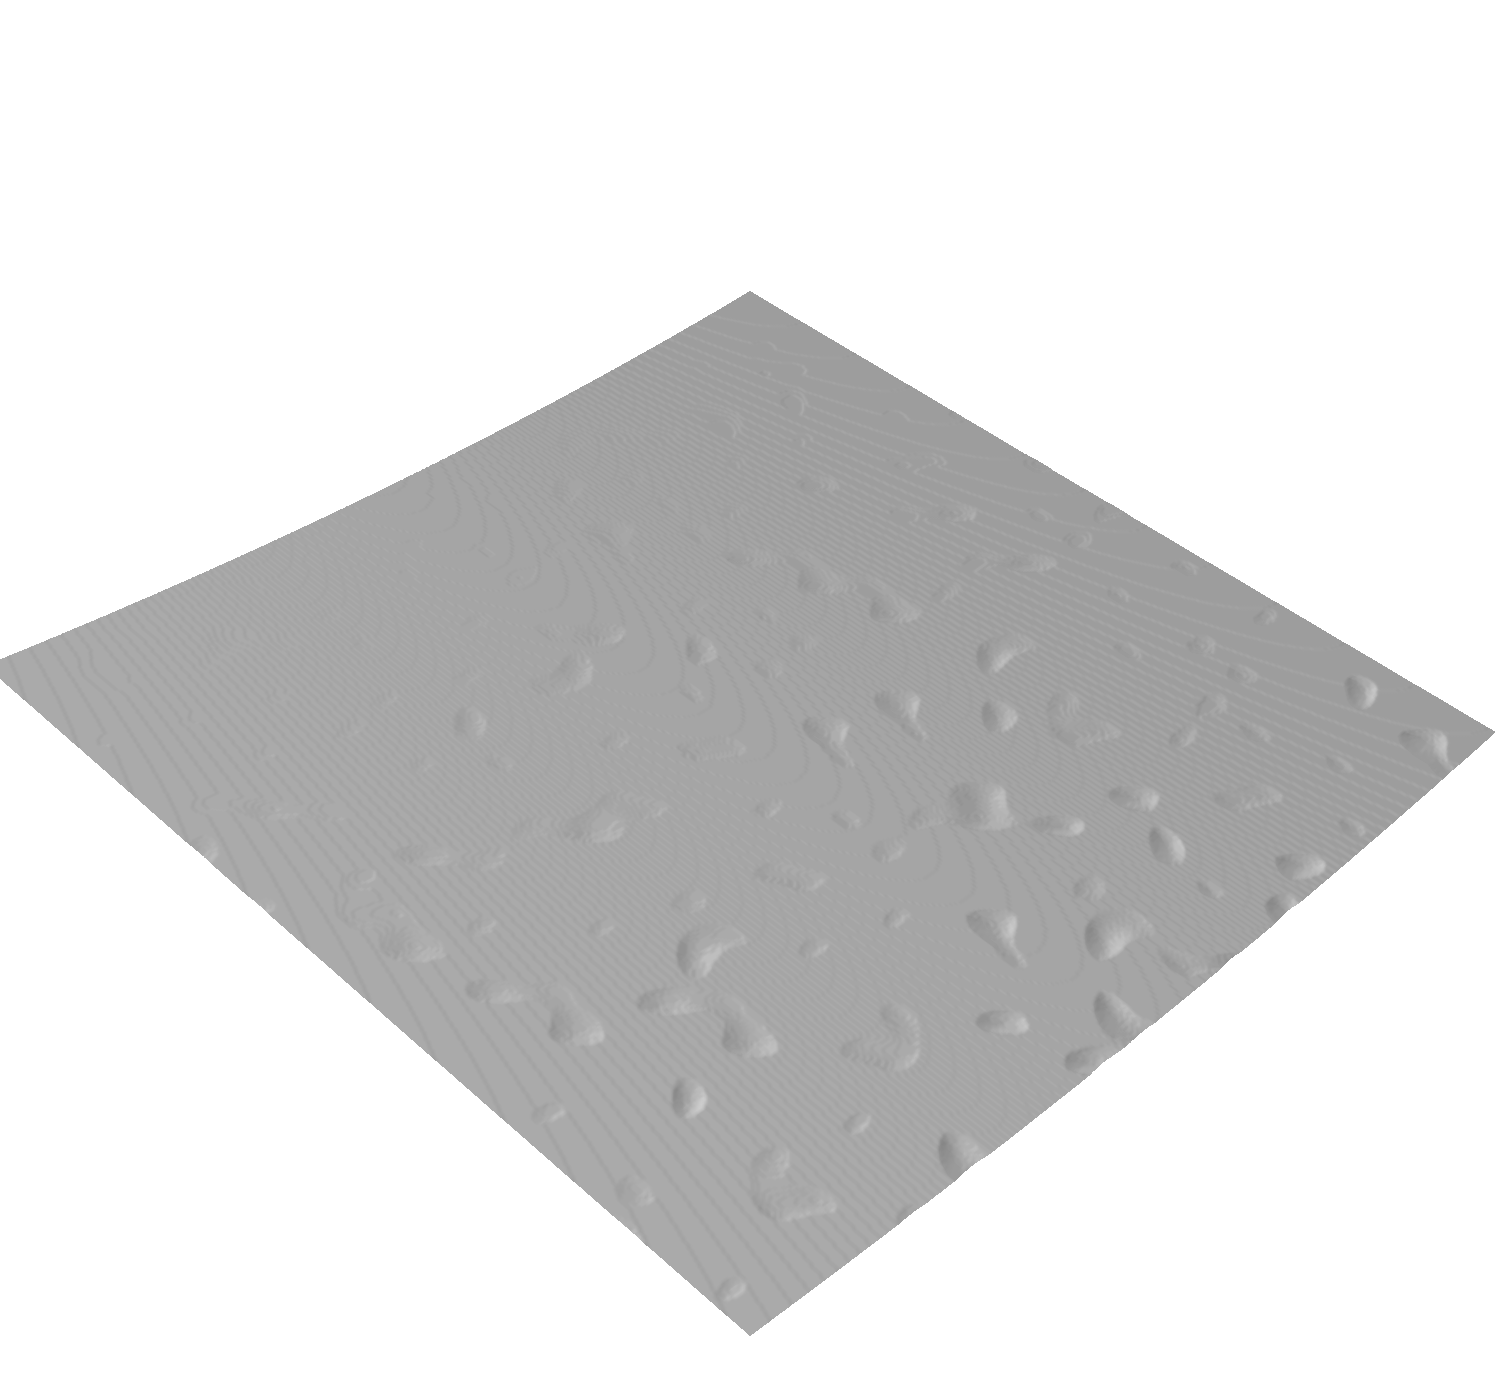
\includegraphics[width=\textwidth]{../img/hm3d/slope_rocks1.png}
            \caption{\emph{slope\_rocks1}}
        \end{subfigure}    
    \label{fig: heightmaps}
    \caption{Slopes maps.}
\end{figure}

\todo[inline]{3d rendered heightmap from Blender should visualize better the idea}
\begin{figure}[H]
    \centering
        \begin{subfigure}[b]{0.45\textwidth}
            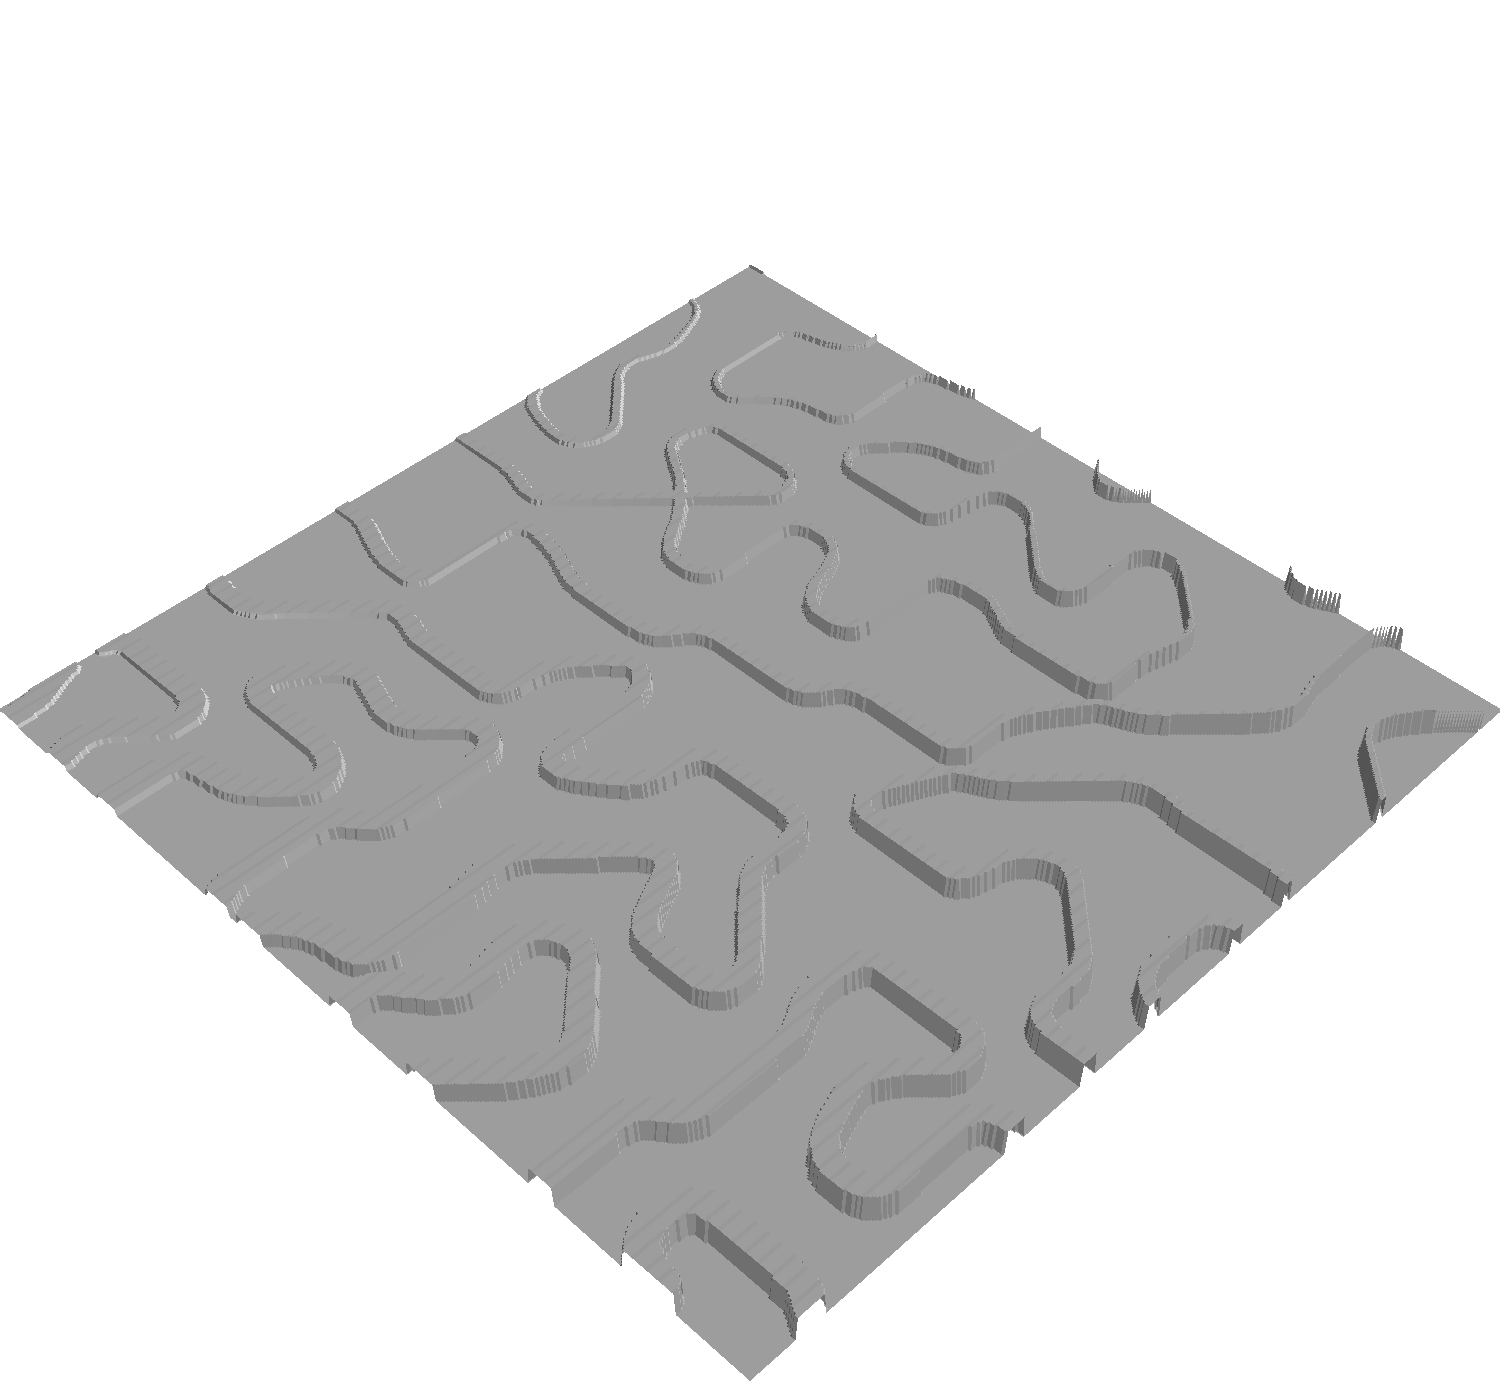
\includegraphics[width=\textwidth]{../img/hm3d/bars1.png}
            \caption{\emph{bars1}}
        \end{subfigure}
        \begin{subfigure}[b]{0.45\linewidth}
            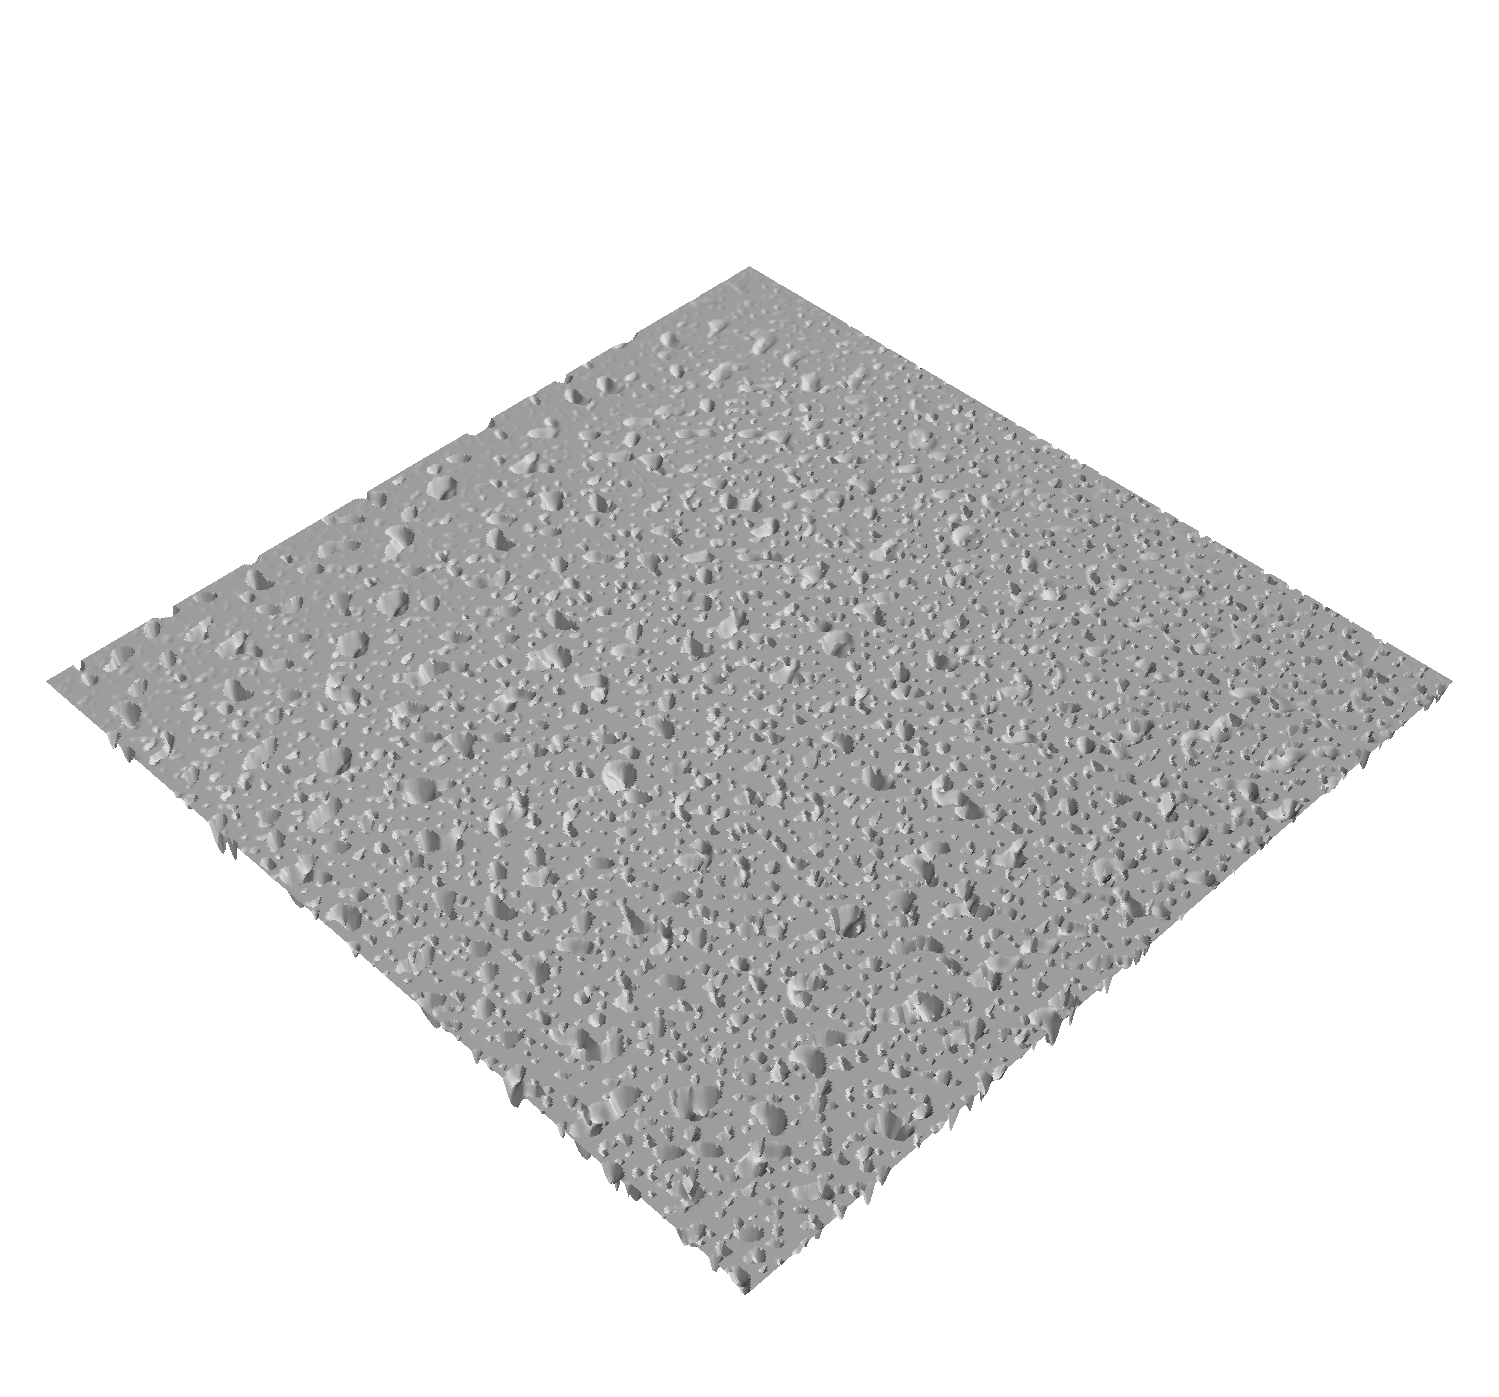
\includegraphics[width=\textwidth]{../img/hm3d/holes1.png}
            \caption{\emph{holes1}}
            \end{subfigure}    
          \begin{subfigure}[b]{0.45\textwidth}
            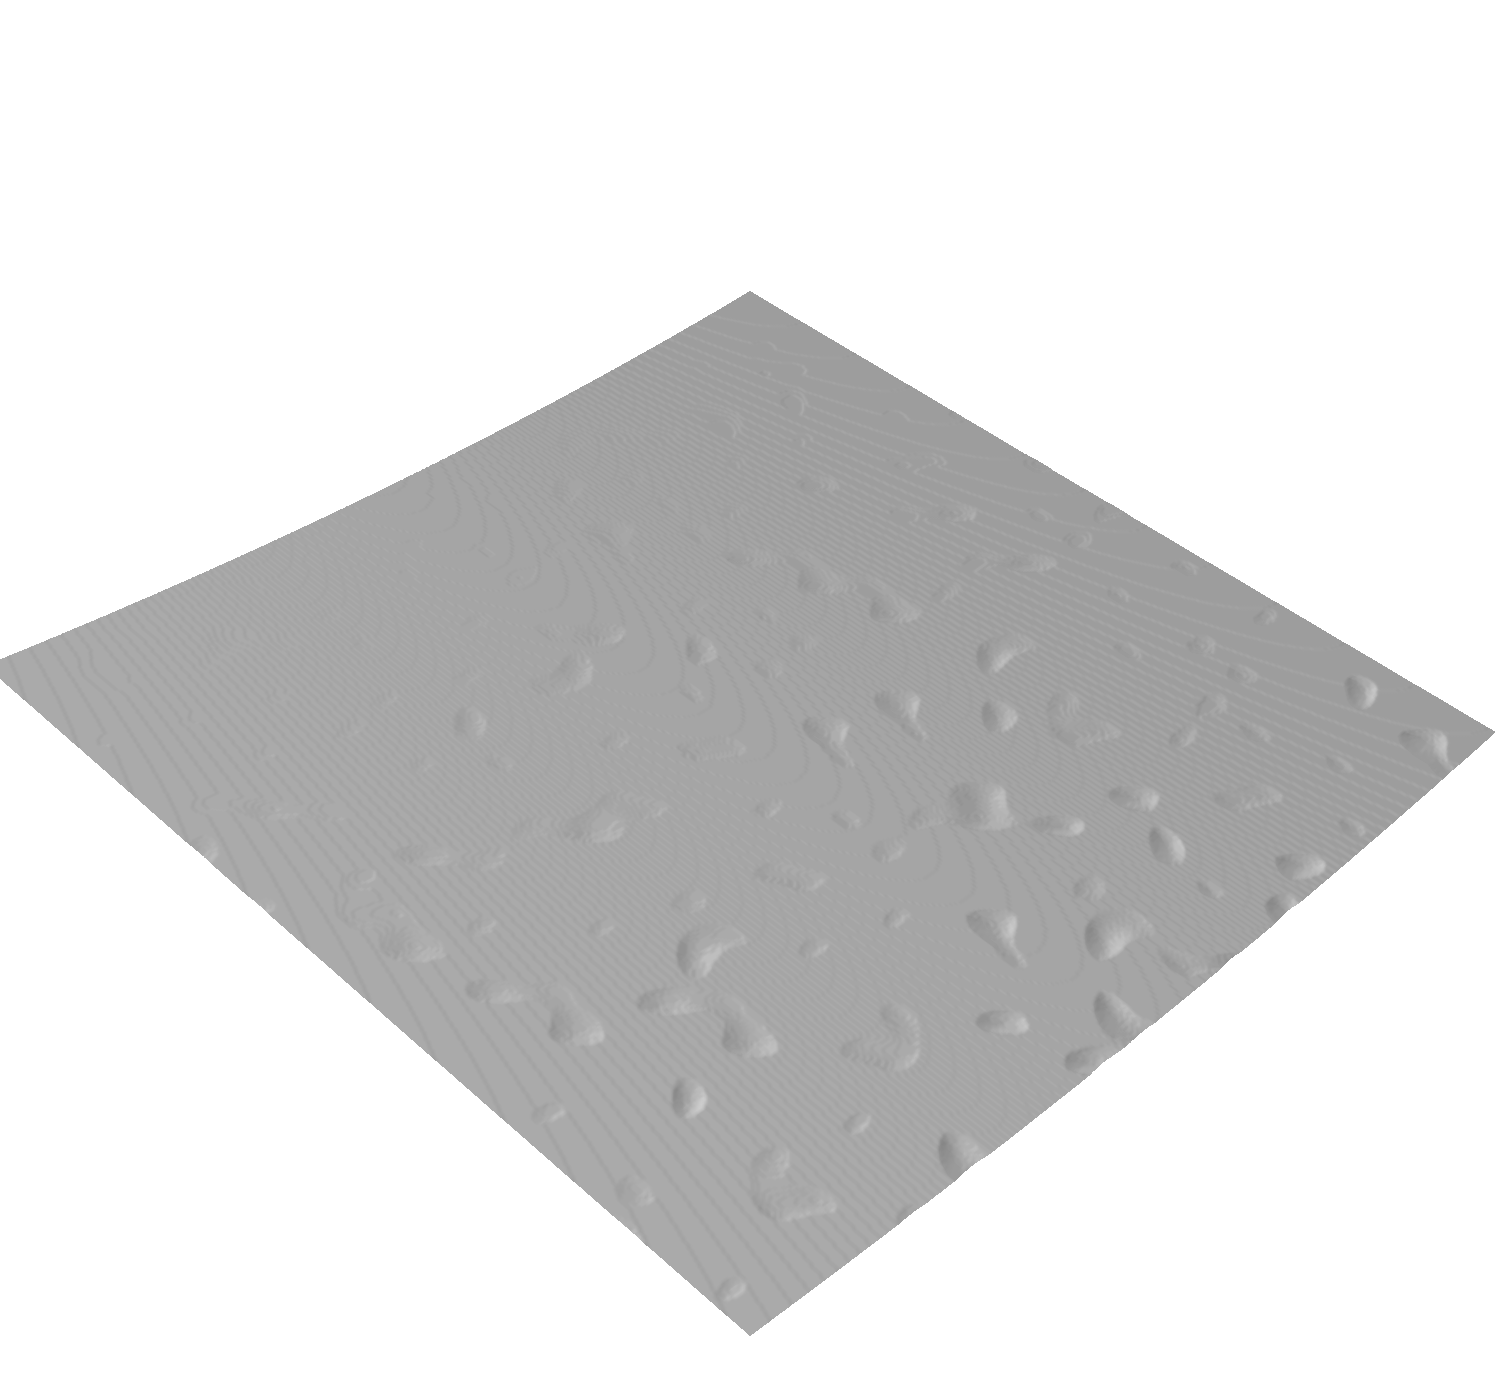
\includegraphics[width=\textwidth]{../img/hm3d/slope_rocks1.png}
            \caption{\emph{slope\_rocks1}}
        \end{subfigure}    
        \begin{subfigure}[b]{0.45\textwidth}
            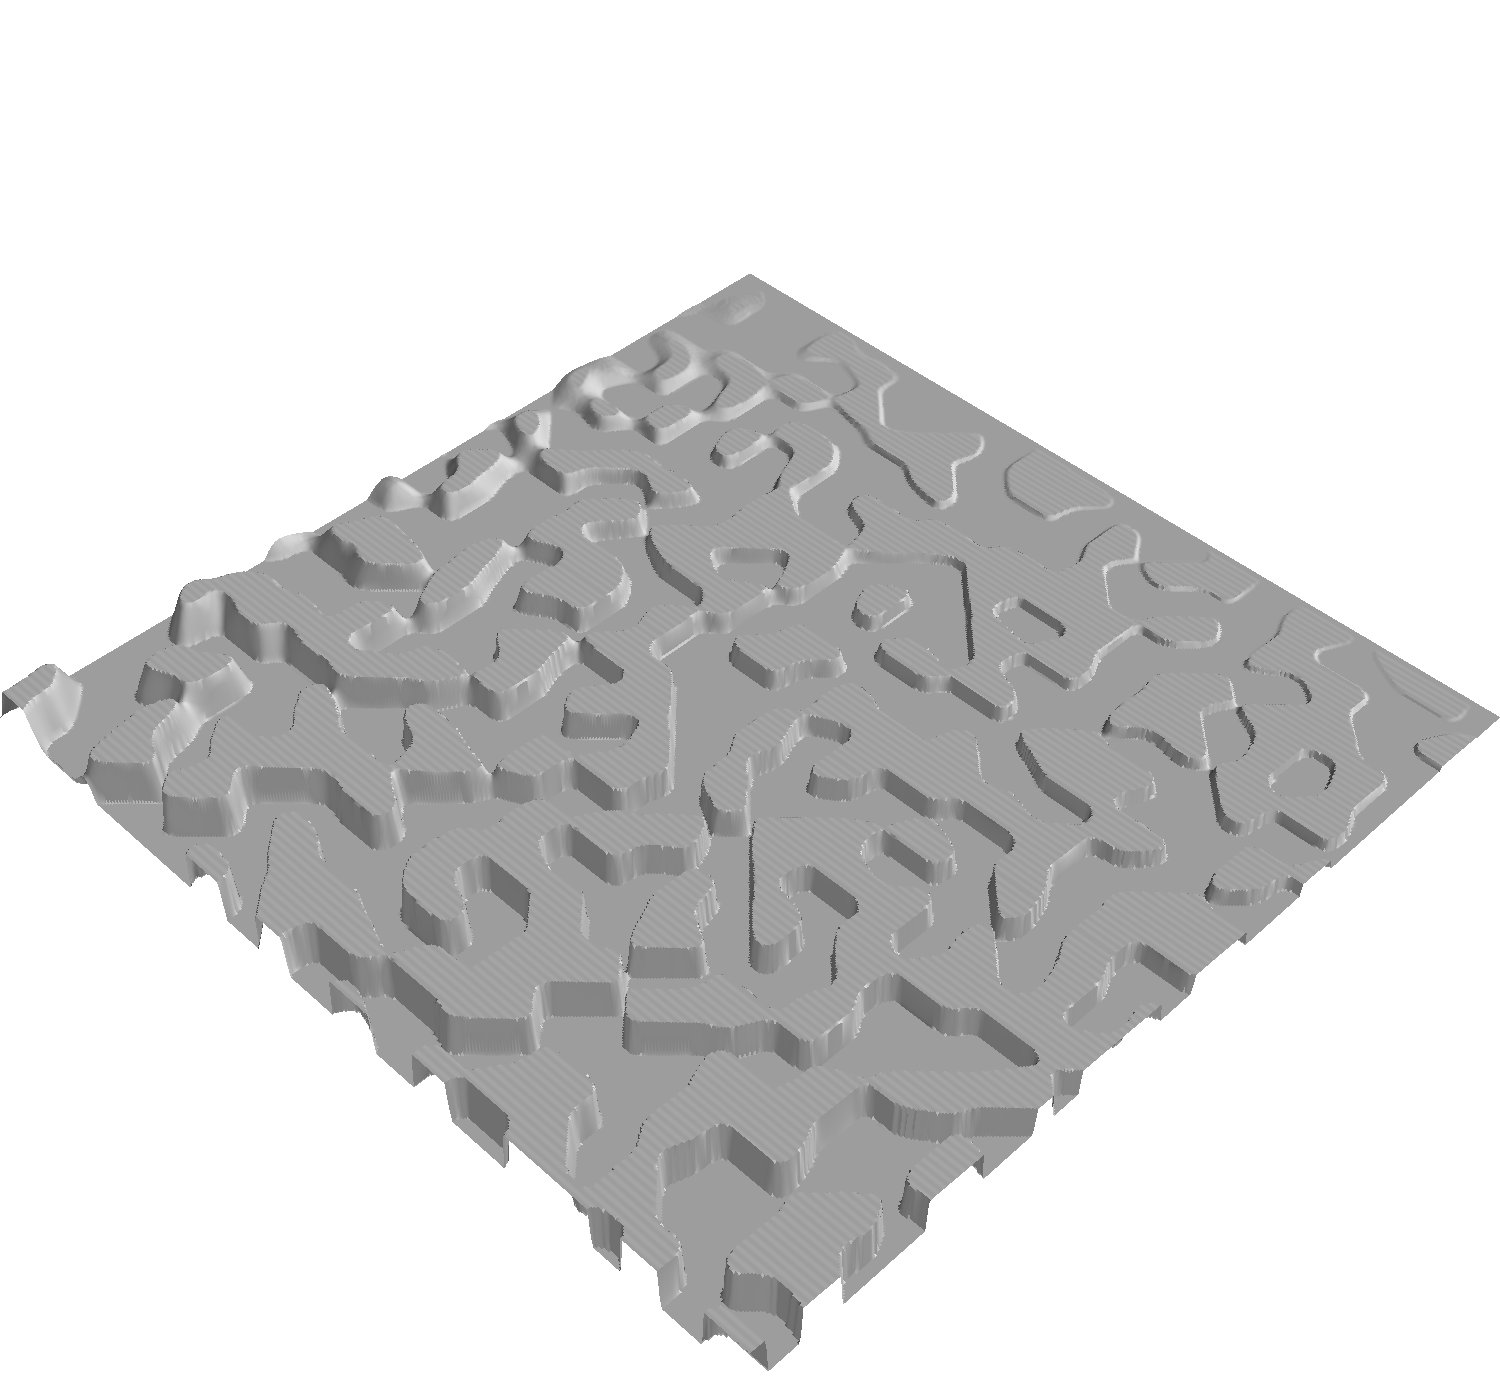
\includegraphics[width=\textwidth]{../img/hm3d/steps1.png}
            \caption{\emph{steps1}}
        \end{subfigure}    
    \label{fig: heightmaps}
    \caption{Some of the synthetic heightmaps}
\end{figure}
\todo[inline]{blender maps are better but I need to write a proper code to generate them}
\subsubsection{Simulator}
We used Webots to move \emph{Krock} on the genereted terrain. The robot controlled was implemented by EPFL \todo{cite them?} and handed to IDSIA \todo{cite?}. The controller implements a ROS' node to publish \emph{Krock} status including its pose at a rate of $250hz$. We decide to reduce it $50hz$ by using ROS build it \texttt{throttle} command. 
To load the map into the simulator we had to convert it to Webots's \emph{.wbt} file. Unfortunately, the simulator lacks support for heightmap so we had to use a script to read the image and perform the conversion.

To communicate with the simulator, Webots exposes a wide number of ROS services, similar to HTTP endpoints, with which we can communicate. The client can use the services to get the value of a field of a Webots' Node, for example, if we want to get the terrain height, we have to ask for the field value \texttt{height} from \texttt{TERRAIN} node. In addition, to call one service, we first have to get the correct type of message we wish to send and then we can call it. We decided to implement a little library called \href{https://github.com/FrancescoSaverioZuppichini/Master-Thesis/tree/master/core/utilities/webots2ros}{\texttt{webots2ros}} to hide all the complexity needed to fetch a field value from a node.

We also implement one additional library called \href{https://github.com/FrancescoSaverioZuppichini/Master-Thesis/tree/master/core/simulation/agent}{\texttt{Agent}} to create reusable robot's interfaces independent from the simulator. The package supports callbacks that can be attached to each agent adding additional features. Finally, we used \emph{Gym} \cite{gym}, a toolkit to develop and evaluate reinforcement learning algorithms, to define our environment. Due to the library's popularity,  the code can easily be shared with other researches or we may directly experiment with already made RL algorithm in the future without changing the code.

\subsubsection{Simulation}
To collect \emph{Krock}'s interaction with the environment, we spawn the robot on the ground and let it move forward for $t$ seconds. We repeat this process $n$ times per each map.
    Unfortunately, spawning the robot is not a trivial task. In certain maps, for instance, \emph{bars1}, we must avoid spawning on an obstacle otherwise the run will be ruined by \emph{Krock} getting stuck at the beginning. To solve the problem, we define a random spawn strategy used in most of the maps without big obstacles such as \emph{slope\_rocks}, and a flat ground spawn strategy for the others. The random spawn just selects a random position and rotation for the robot. On the other hand, the flat ground strategy first selects suitable spawn positions by using a sliding window on the heightmap of size equal \emph{Krock}'s footprint and check if the mean pixel value is lower than a small threshold. If so, we store the center coordinates of the patch. Intuitively, if a patch is flat the mean value will be close to zero.
    
We clustered those points with K-Means in $k$ clusters where $k$ is the number of spawning points we need, in our case fifty. By clustering, we guarantee to cover all region of the map. The following picture shows this strategy on \emph{bars1}. 
\begin{figure}[H]
    \begin{subfigure}[b]{0.5\textwidth}
        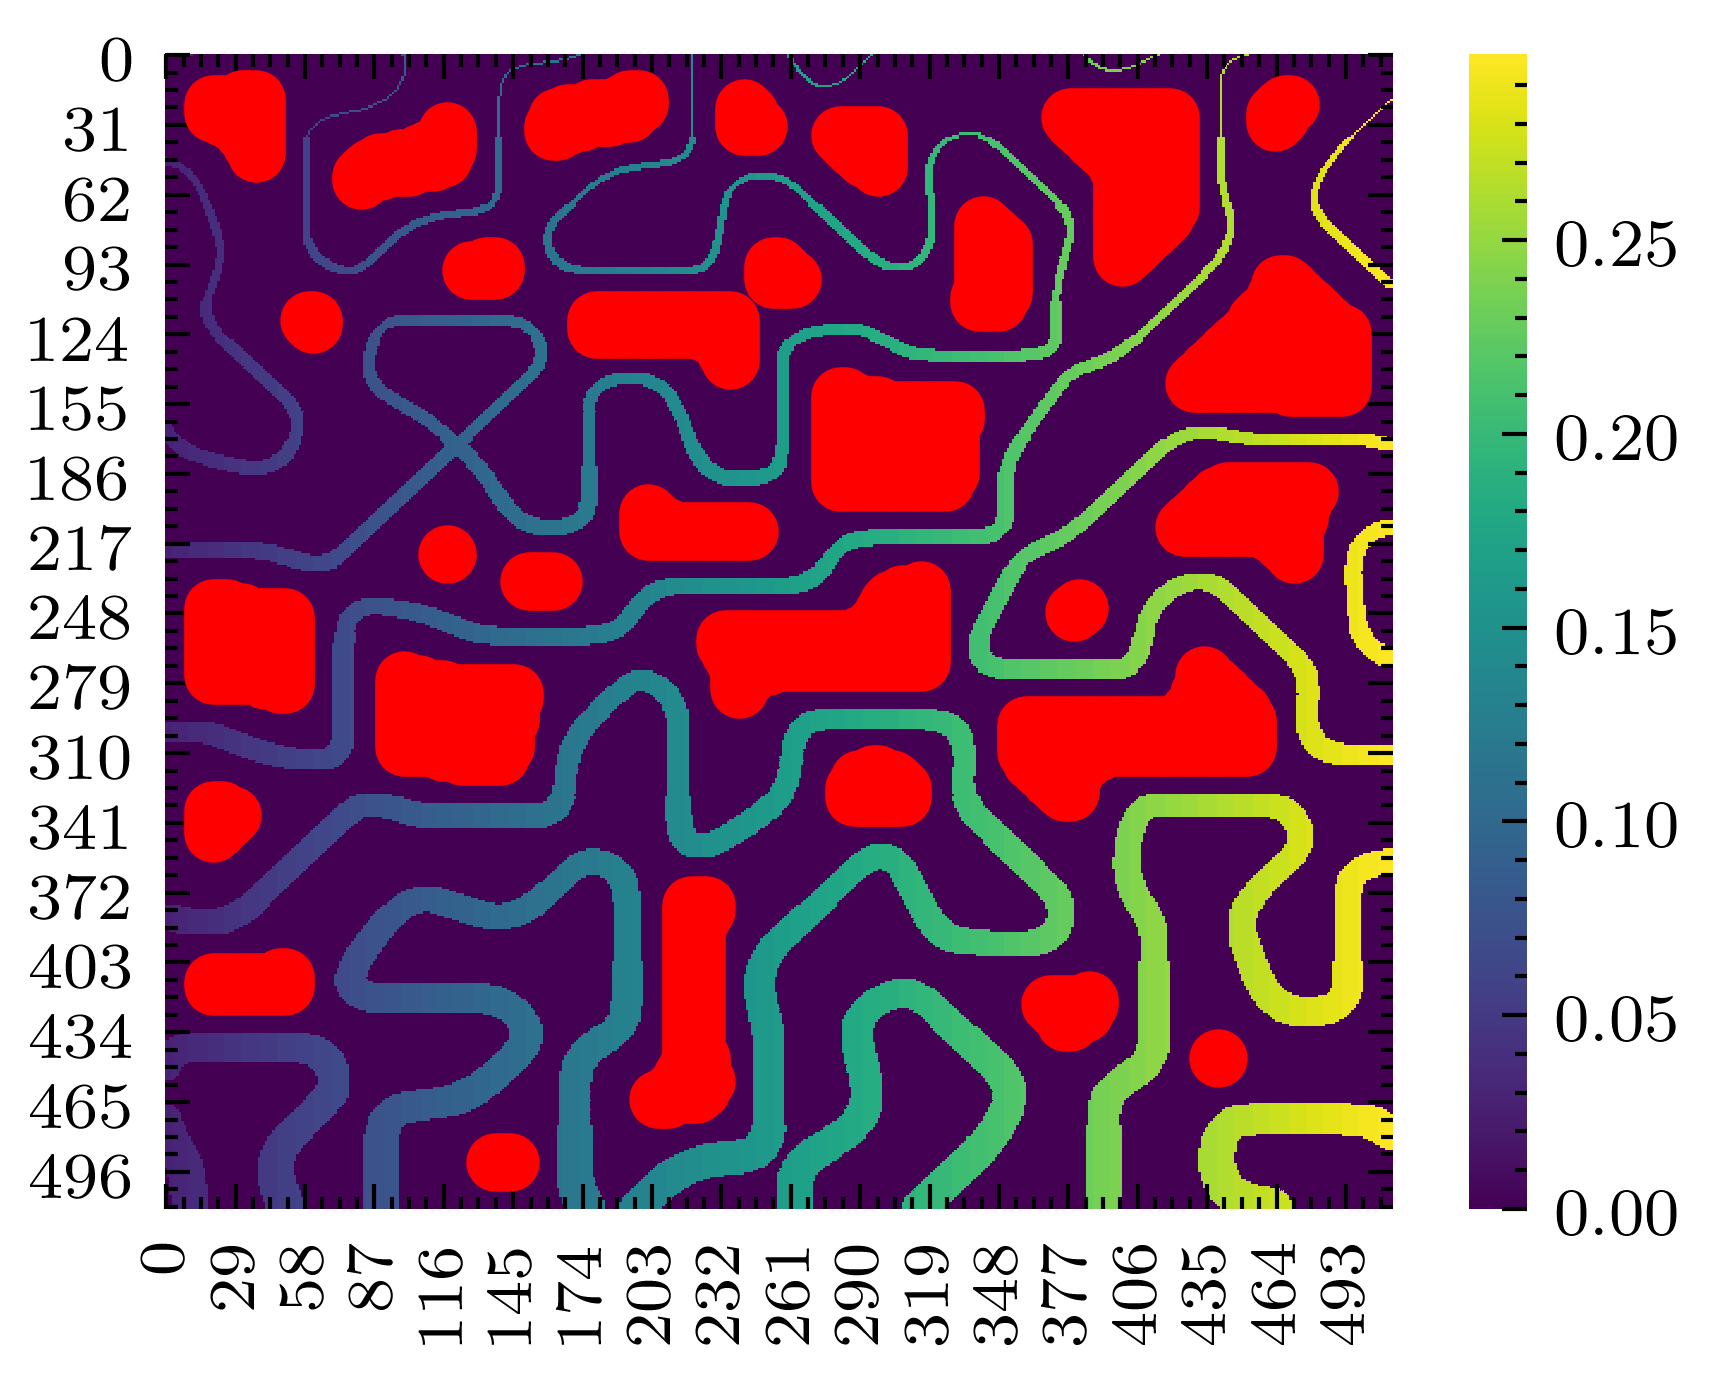
\includegraphics[width=\textwidth]{../img/3/spawn/flat-spawn-10.png}
        \caption{Flat regions}
    \end{subfigure}
    \begin{subfigure}[b]{0.5\textwidth}
        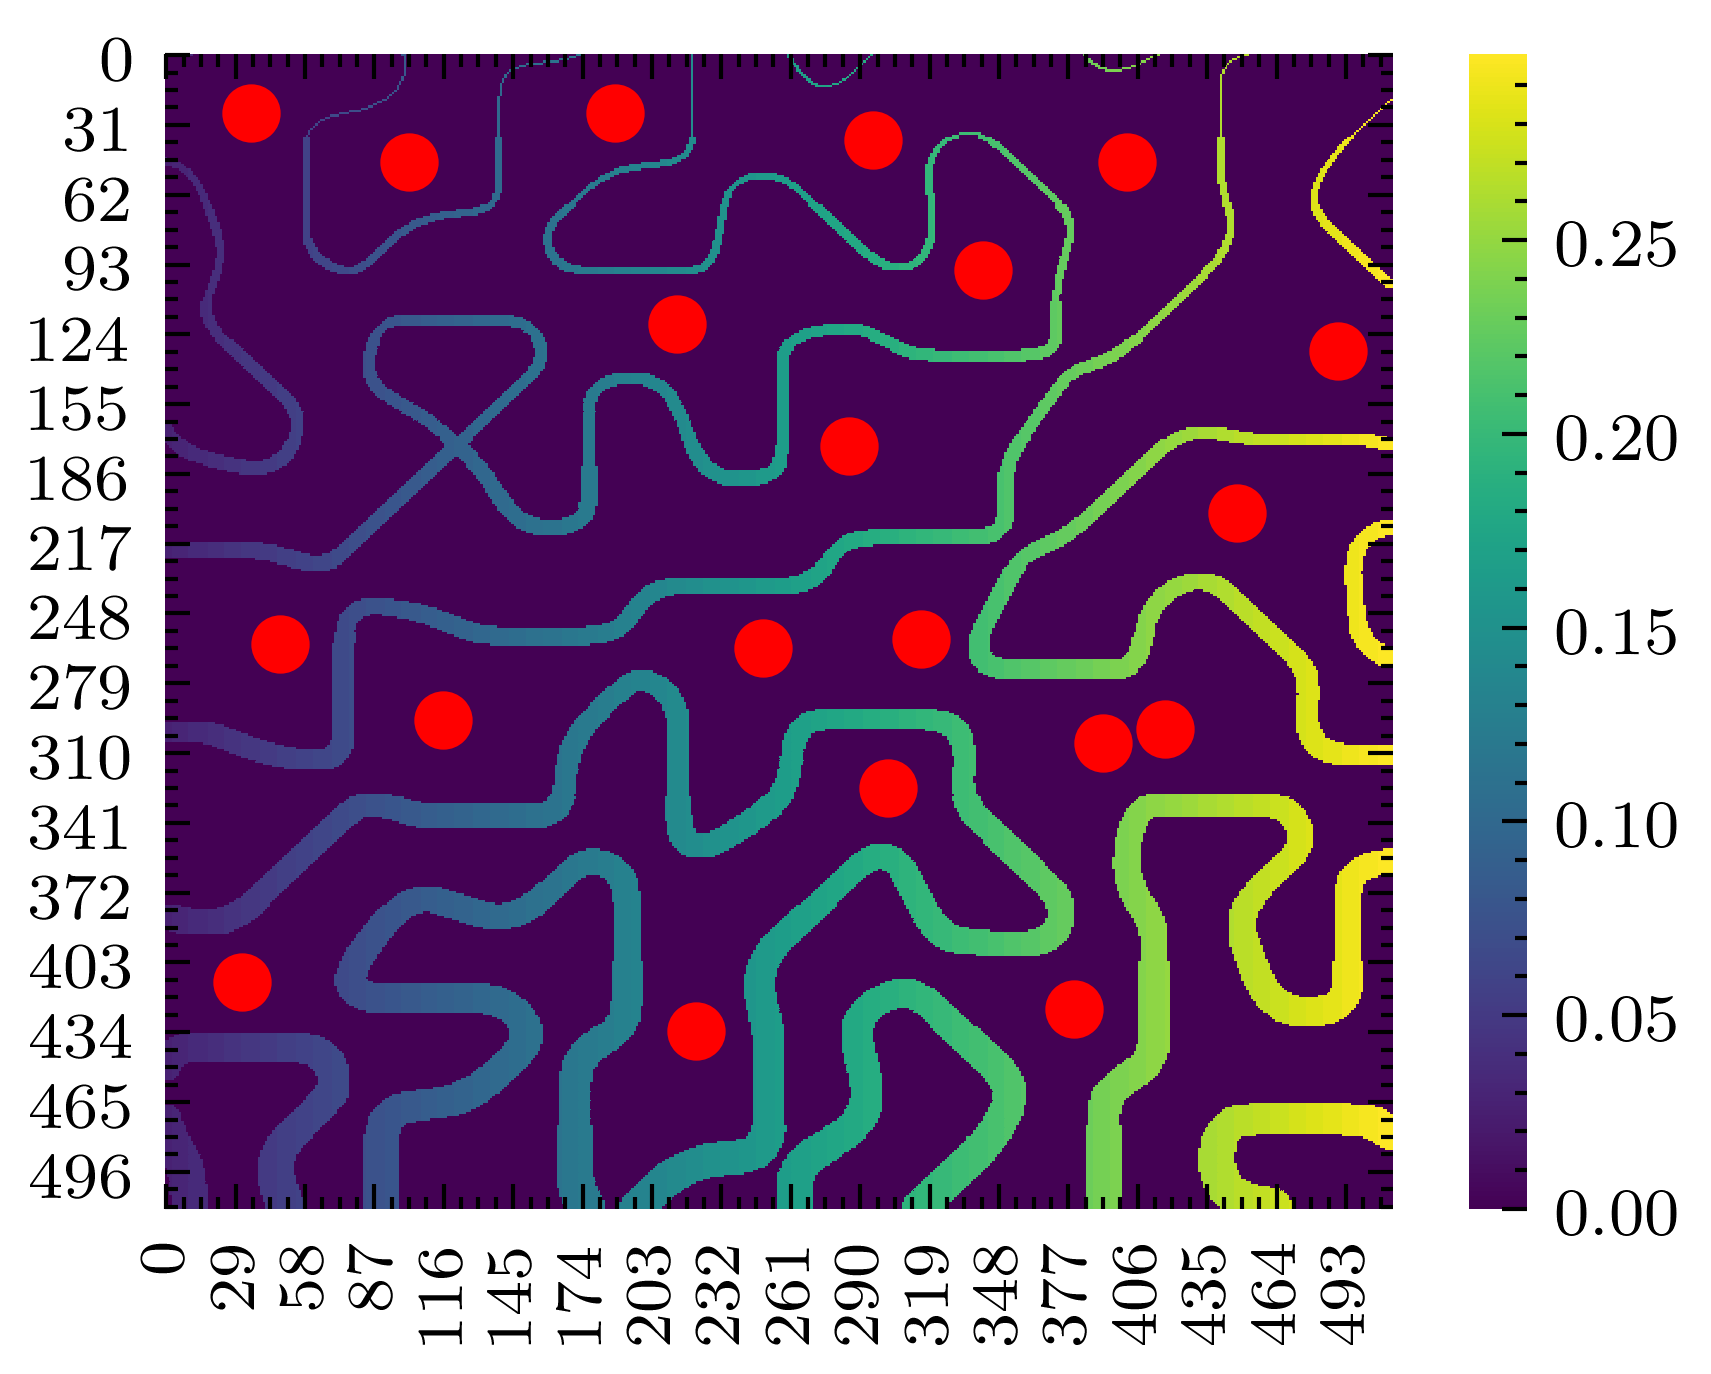
\includegraphics[width=\textwidth]{../img/3/spawn/spawn-10.png}
        \caption{K-Means with $k=20$}
    \end{subfigure}  
\label{fig: spawn-strat}
\caption{Examples of the spawning selection process (marked as red blobs) for the map \emph{bars1} }   
\end{figure}
The following table shows the maps configuration used in the simulator.
\begin{table*}[h]
    \centering
    \ra{1.2}
    
    \begin{tabular}{@{}llccccc@{}}
      \toprule
      & Map & Height(m) & Spawn & Texture & Simulations & max time(s) \\ 
      \hline
      &\multirow{3}{*}{\emph{bumps0}} & \multirow{3}{*}{2} & \multirow{3}{*}{random} &- & \multirow{3}{*}{50} & \multirow{3}{*}{10} \\
      &&&& rocks1 &  &  \\ 
      &&&& rocks2 &  &  \\ 
      \hline
      &\multirow{3}{*}{\emph{bumps1}} & \multirow{3}{*}{1} & \multirow{3}{*}{random}& - & \multirow{3}{*}{50} & \multirow{3}{*}{10} \\
      &&&& rocks1 &  &  \\ 
      &&&& rocks2 &  &  \\ 
      \hline
      &\multirow{4}{*}{\emph{bumps2}} & \multirow{3}{*}{1} & \multirow{4}{*}{random} &- & \multirow{3}{*}{50} & \multirow{4}{*}{10} \\
      &&&& rocks1 &  &  \\ 
      &&&& rocks2 &  &  \\ 
      && 2 && - &  &  \\ 
      \hline
      &\multirow{3}{*}{\emph{bumps3}} & \multirow{3}{*}{1}& \multirow{3}{*}{random} & - & \multirow{4}{*}{50} & \multirow{3}{*}{10} \\
      &&&& rocks1 &  &  \\ 
      &&&& rocks2 &  &  \\ 
      \hline
      &\emph{steps1} & 1 &random & - & \multirow{3}{*}{50} &  \multirow{3}{*}{10} \\
      &\emph{steps2} & 1 &flat & - &  &  \\
      &\emph{steps3} & 1 &random & - &  &  \\
      \hline
      &\emph{rails1} & 1 & \multirow{3}{*}{flat} &\multirow{3}{*}{-} & \multirow{3}{*}{50} & 20 \\
      &\emph{rails2} & 1 &&  &  & \multirow{2}{*}{10} \\
      &\emph{rails3} & 1 &&  &  &  \\
      \hline
      &\multirow{2}{*}{\emph{bars1}} & 1 & \multirow{3}{*}{flat} & - & \multirow{3}{*}{50} & \multirow{3}{*}{10} \\
      && 2 &  & - &  &  \\
      &\emph{bars3} & 1 & & - &  &  \\
      \hline
      &\multirow{2}{*}{\emph{ramp0}} & \multirow{2}{*}{1} & \multirow{2}{*}{random} & rocks1 & 50 & \multirow{2}{*}{10} \\
      &&&& rocks2 & 50 &  \\
      \hline
      &\multirow{3}{*}{\emph{ramp1}} & 3 & \multirow{3}{*}{random} & \multirow{3}{*}{-} & \multirow{3}{*}{50} & \multirow{3}{*}{10} \\
      && 4 &&&& \\
      && 5 &&&& \\
      \hline 
      &\multirow{3}{*}{\emph{slope\_rocks1}} & 3 & \multirow{3}{*}{random} & \multirow{3}{*}{-} & \multirow{3}{*}{50} & \multirow{3}{*}{10} \\
      && 4 &&&& \\
      && 5 &&&& \\
      \bottomrule   
  
    \end{tabular}
    \caption{Maps configuration used in the simulator.}
  
  \end{table*}
  


\subsection{Postprocessing}
We now need to extract the patches for each pose $p_t$ of \emph{Krock} and compute the advancement for a given time window. To create the post-processing pipeline, we create an easy to use API called \href{https://github.com/FrancescoSaverioZuppichini/Master-Thesis/tree/master/core/utilities/pipeline}{\texttt{pipeline}} to define a cascade stream of function that is applied one after the other using a multi-thread queue to speed-up the process
\subsubsection{Parse simulation data}
First, we turn each \emph{.bag} file into a pandas dataframe and cache them into \emph{.csv} files. We used \href{https://github.com/aktaylor08/RosbagPandas}{\texttt{rosbag\_pandas}}, an open source library we ported to python3, to perform the conversion.
Then, we load the dataframes with the respective heightmaps and start the data cleaning process. We remove the rows corresponding tp the first second of the simulation time to account for the robot spawning time. Then we eliminate all the entries where the \emph{Krock} pose was near the edges of a map, we used a threshold of $22$ pixels since we notice  \emph{Krock} getting stuck in the borders of the terrain during a simulation. 
After cleaning the data, we convert \emph{Krock}quaternion rotation to Euler notation using the \href{https://duckduckgo.com/?q=ros+tf&atb=v154-1__&ia=web}{\texttt{tf}} package from ROS. Then, we extract the $\sin$ and $\cos$ from the Euler orientation last component and store them in a column.
Before caching again the resulting dataframes into \emph{.csv} files, we convert the robot's position into heightmap's coordinates used later to crop the correct region of the map.

Finally, we load again the last stage and compute the advancement by projecting the pose's position, $x$ and $y$, in the current line. Then, we select a time window according to the store rate, for if we select two seconds we need to multiply the rate by two, so $50*2=100$ since \emph{Krock} published with a $50hz$ frequency. Once the time window is defined, we project $x$ and $y$ on the current line The Robot Operating System (ROS) \cite{ROS} is a flexible framework for writing robot software. It is \emph{de facto} the industry and research standard framework for robotics due to its simple yet effective interface that facilitates the task of creating a robust and complex robot behavior regardless of the platforms. ROS works by establishing a peer-to-peer connection where each \emph{node} is to communicate between the others by exposing sockets endpoints, called \emph{topics}, to stream data or send \emph{messages}. used the $\sin$ and $\cos$ values calculated before to get the advancement.
\subsubsection{Extract patches}
To create the patches, we first discover the maximum advancement for one second by running some simulations of \emph{Krock} on flat ground and averaging the advancement. For our robot, the maximum speed is $33cm/s$ Then, we multiply the maximum displacement by the number of seconds we are interested in. We can now crop the corresponding region in the heightmap by including the whole \emph{Krock}'s footprint and the maximum advancement. The following figure visualizes the patch extraction process. 
\todo[inline]{figure that shows Krock somewhere with the patch bounding boxed}. Lastly, we create a final dataframe containing the map coordinates, the advancement, and the patches paths for each simulation and store them to disk as \emph{.csv} files. 

The whole pipeline takes less than one hour to run the first time with 16 threads, and, once it is cached, less than fifteen minutes to extract the patches. 

Once we extract the patches, we can always re-compute the advancement without re-running the whole pipeline. The next figure show proposed pipeline.
\begin{figure}[H] 
\centering
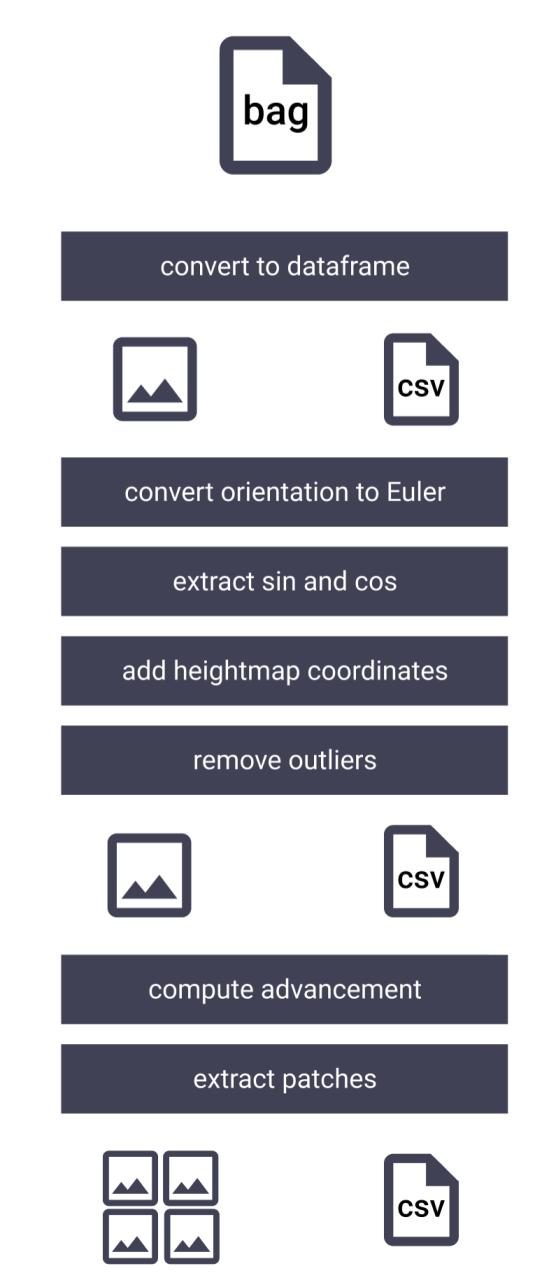
\includegraphics[width=0.4\textwidth]{../img/postprocessing-pipeline.jpg}
\caption{Postprocessing pipeline flow from top to bottom}
\label{fig: postprocessing-pipeline}
\end{figure}
\todo[inline]{add arrows!}
\subsection{Estimator}
In this section we shows the adopted models' architecture.
\subsubsection{Vanilla Model}
\subsubsection{ResNet}
We decide to use a Residual Network, ResNet \cite{he2015deep}, variant. Residual networks are deep convolutional
networks consisting of many stacked \" Residual Units \". Intuitively, the residual unit allows the input of a layer to contribute to the next layer's input by being added to the current layer's output. Due to possible different features dimension, the input must go through and identify map to make the addition possible. This allows a stronger gradient flows and mitigates the degradation problem. A \"Residual Units \" is composed by a two $3x3$ \emph{Convolution}, \emph{Batchnorm} \cite{ioffe2015batch} and a \emph{Relu} blocks. Formally, it is defined as: 
\begin{equation}
    \mathbf{y}=\mathcal{F}\left(\mathbf{x},\left\{W_{i}\right\}\right)+h(\mathbf{x})
    \label{eq : resnet}
\end{equation}
Where, $x$ and $y$ are the input and output vector of the layers considered. The function $\mathcal{F}\left(\mathbf{x},\left\{W_{i}\right\}\right)$ is the residual mapping to be learn and $h$ is the identity mapping. The next figure visualises the equation.

\begin{figure}[H]
    \centering
    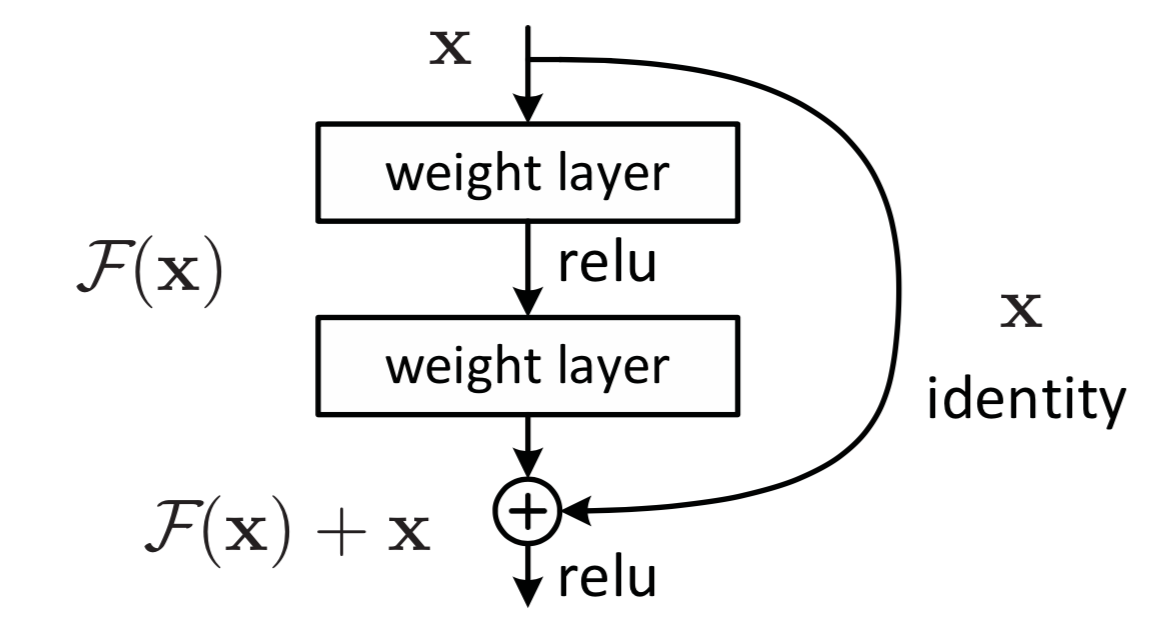
\includegraphics[scale=0.3]{../img/implementation/estimator/resnet_block.png}
    \caption{\emph{Resnet} block \cite{he2015deep}}
\end{figure}
When the input and output shapes mistmatch, the \emph{identity map} is applyed to the input as a $3x3$ Convolution with a stride of 2 to mimic the polling operator. A single block is composed by a $3x3$ \emph{Convolution}, \emph{Batchnorm} and a \emph{Relu} activation function. 
\subsubsection{Preactivation}
Following the recent work of He et al. \cite{he2015identity} we adopt \emph{pre-activation} in each block.\emph{Pre-activation} works by just reverse the order of the operations in a block.

\begin{figure}[H]
    \centering
    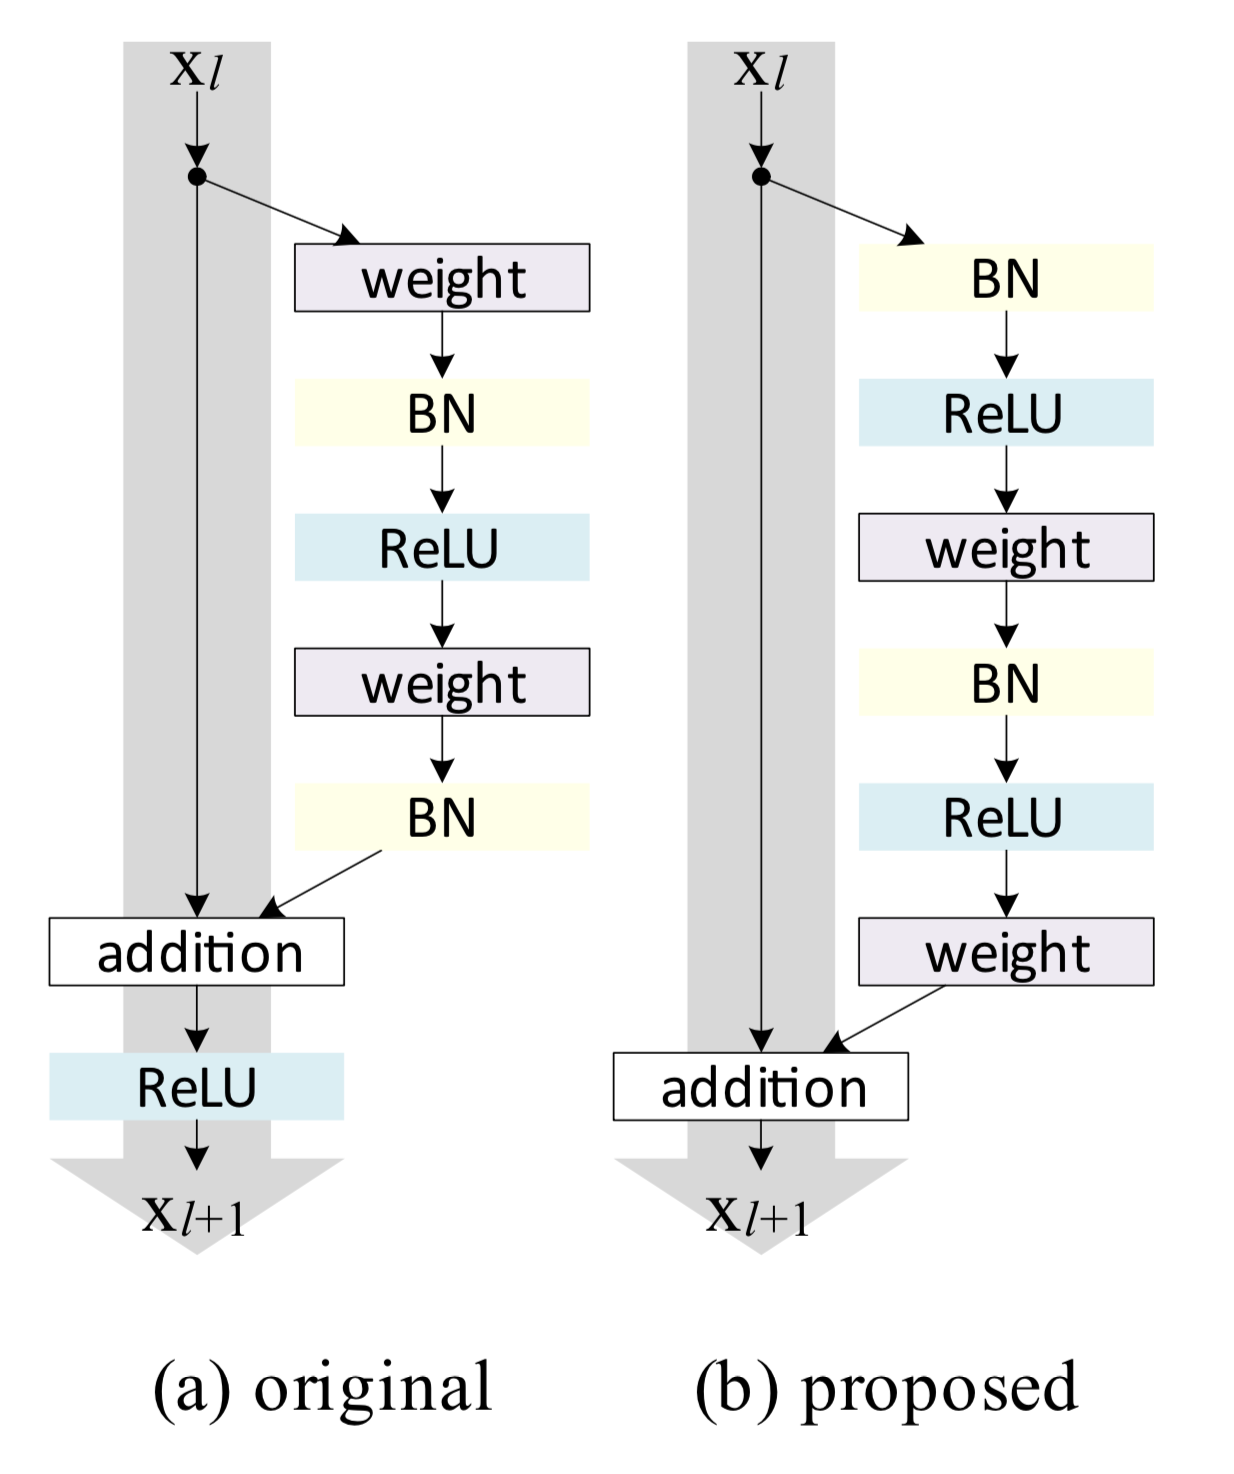
\includegraphics[scale=0.2]{../img/implementation/estimator/preactivation.png}
    \caption{\emph{Preactivation} \cite{he2015identity}}
\end{figure}
\subsubsection{Sqeeze and Excitation}
Finally, we also used the \emph{Squeeze and Excitation} (SE) module \cite{hu2017squeeze}. It is a form of attention that weights the channel of each convolutional operation by learnable scaling factors. Formally, for a given transformation, e.g. Convolution, defined as $\bm{F}_{tr}  : \bm{X} \mapsto \bm{U}$, $\bm{X} \in mathbb{R}^{H' \times W' \times C'}$, $\bm{U} \in \mathbb{R}^{H \times W \times C}$, the SE module first squeeze the information by using average pooling, $\bm{F}_{sq}$, the it excitates them using learnable weights, $\bm{F}_{ex}$ and finally, adaptive recalibration is performed, $\bm{F}_{scale}$.
The next figure visualises the SE module.
\begin{figure}[H]
    \centering
    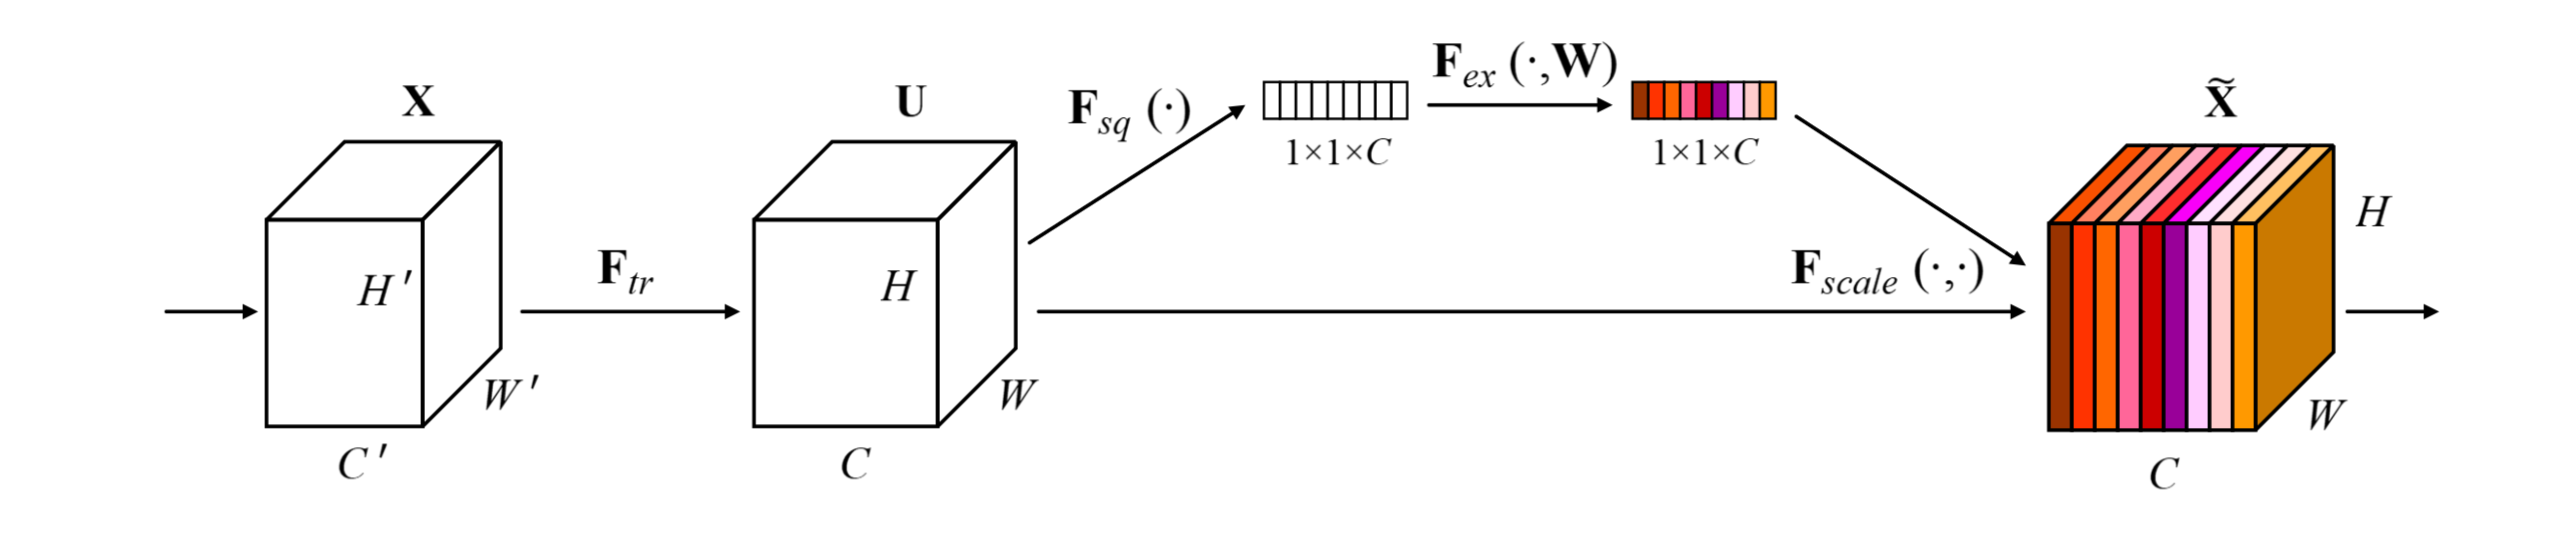
\includegraphics[width=\linewidth]{../img/implementation/estimator/se.png}
    \caption{\emph{Squeeze and Excitation} \cite{hu2017squeeze}}
\end{figure}
\subsubsection{Micro resnet}
Our network differs is composed by $n$ ResNet blocks, a depth of $d$ and a channel incrementing factor of $2$. We evaluate $n=[1,2], d=3$ with and without SE module all with a starting channel size of $16$ and finally select $n=1$ and $d=3$ with a starting channel size of $16$, we called this model architecture \emph{micro-resnet}. 

\begin{table}[H]
    \centering
    \ra{1.2}
        \begin{tabular}{@{}lc|cccc@{}}
        \hline
        & depth   &  \multicolumn{4}{c}{3}  \\ 
        \hline 
        & n   & \multicolumn{2}{c}{1} & \multicolumn{2}{c}{2}\\
        \hline
    \multirow{12}{*}{Layers}
     & &\multicolumn{4}{c}{$3 \ x\ 3,\ 16 \ stride\ 1$} \\ 
     \cline{3-6}
     & &\multicolumn{4}{c}{$2 \ x\ 2$ max-pool} \\ 
     \cline{3-6}
     & & \multicolumn{2}{c}{$\begin{bmatrix}
      3\ x\ 3, & 16 \\
      3\ x \ 3, & 16 \\  
     \end{bmatrix}$ x 1} & \multicolumn{2}{c}{$\begin{bmatrix}
        3\ x\ 3, & 16 \\
        3\ x \ 3, & 16 \\  
       \end{bmatrix}$ x 2}\\ 
       \cline{3-6}
     & & SE & - & SE & -\\ 
     \cline{3-6}
     & & \multicolumn{2}{c}{$\begin{bmatrix}
        3\ x \ 3, & 32 \\
        3\ x\ 3, & 32 \\  
       \end{bmatrix}$ x 1} & \multicolumn{2}{c}{$\begin{bmatrix}
        3\ x\ 3, & 32 \\
        3\ x \ 3, & 32 \\  
       \end{bmatrix}$ x 2} \\
       \cline{3-6}
       & & SE & - & SE & -\\ 
       \cline{3-6}
       & & \multicolumn{2}{c}{$\begin{bmatrix}
        3\ x \ 3, & 64 \\
        3 \ x \ 3, & 64 \\  
       \end{bmatrix}$ x 1} & \multicolumn{2}{c}{$\begin{bmatrix}
        3\ x\ 3, & 64 \\
        3\ x \ 3, & 64 \\  
       \end{bmatrix}$ x 2}\\  
       \cline{3-6}
       & & SE & - & SE & -\\ 
       \cline{3-6}
       & & \multicolumn{4}{c}{average pool, $1$-d fc, softmax} \\ 
       \hline

       Parameters & & TODO & 302,610  & TODO & TODO \\
       \hline
    \end{tabular}
    \caption{\emph{micro-resnet} architectures evaluated}
\end{table}
\todo[inline]{ask omar help to add margin in the rows}
\todo[inline]{add model picture}
\subsubsection{Normalization}
Before feeding the data to the models, we need to make the patches height invariant. This must be done to correctly normalize different patches taken from different maps with different height scaling factor. We subtract the height of the map corresponding \emph{Krock}'s position from the patch to correctly center it. The following figure shows the normalization process on the patch with the square in the middle.
\begin{figure}[H]
    \begin{subfigure}[b]{0.5\textwidth}
        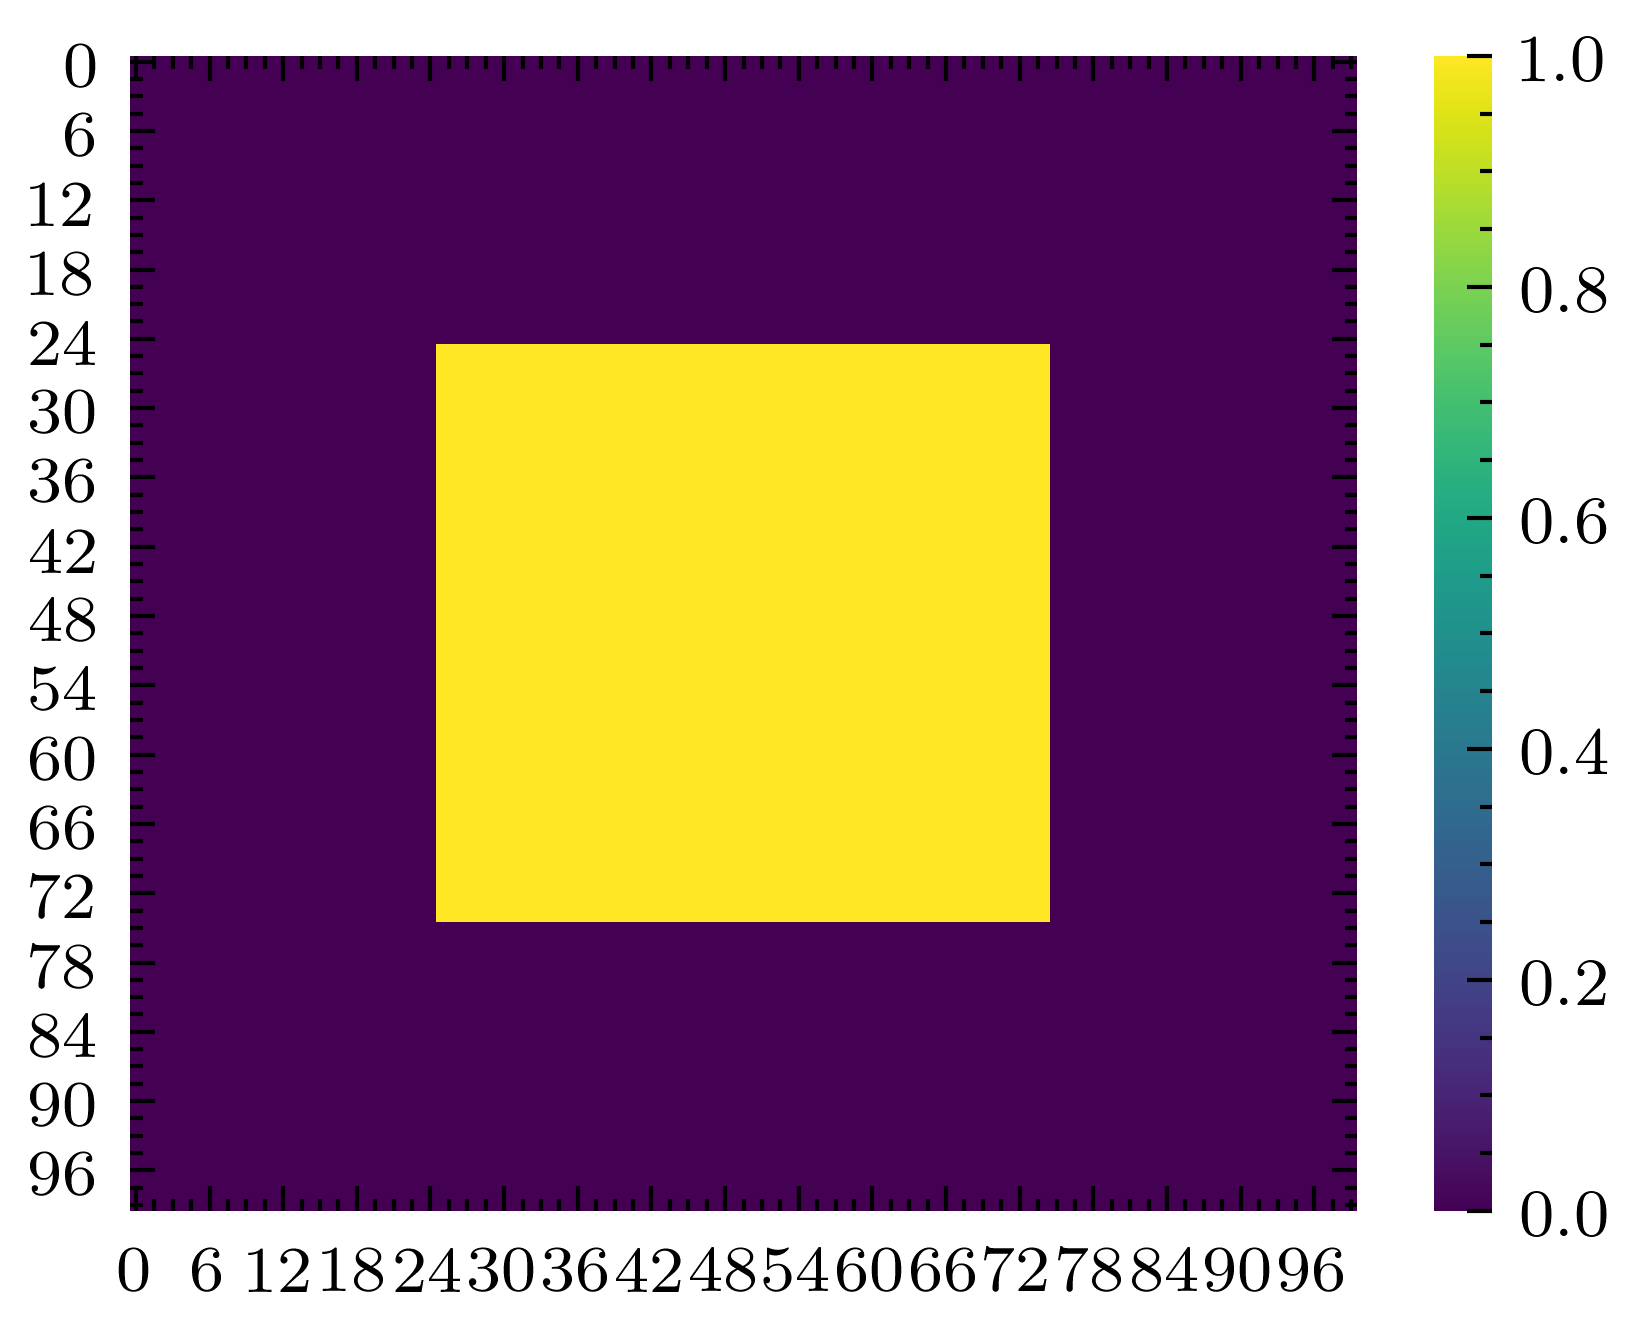
\includegraphics[width=\textwidth]{../img/data-aug/2d/square-middle.png}
        \caption{Input}
    \end{subfigure}
    \begin{subfigure}[b]{0.5\textwidth}
        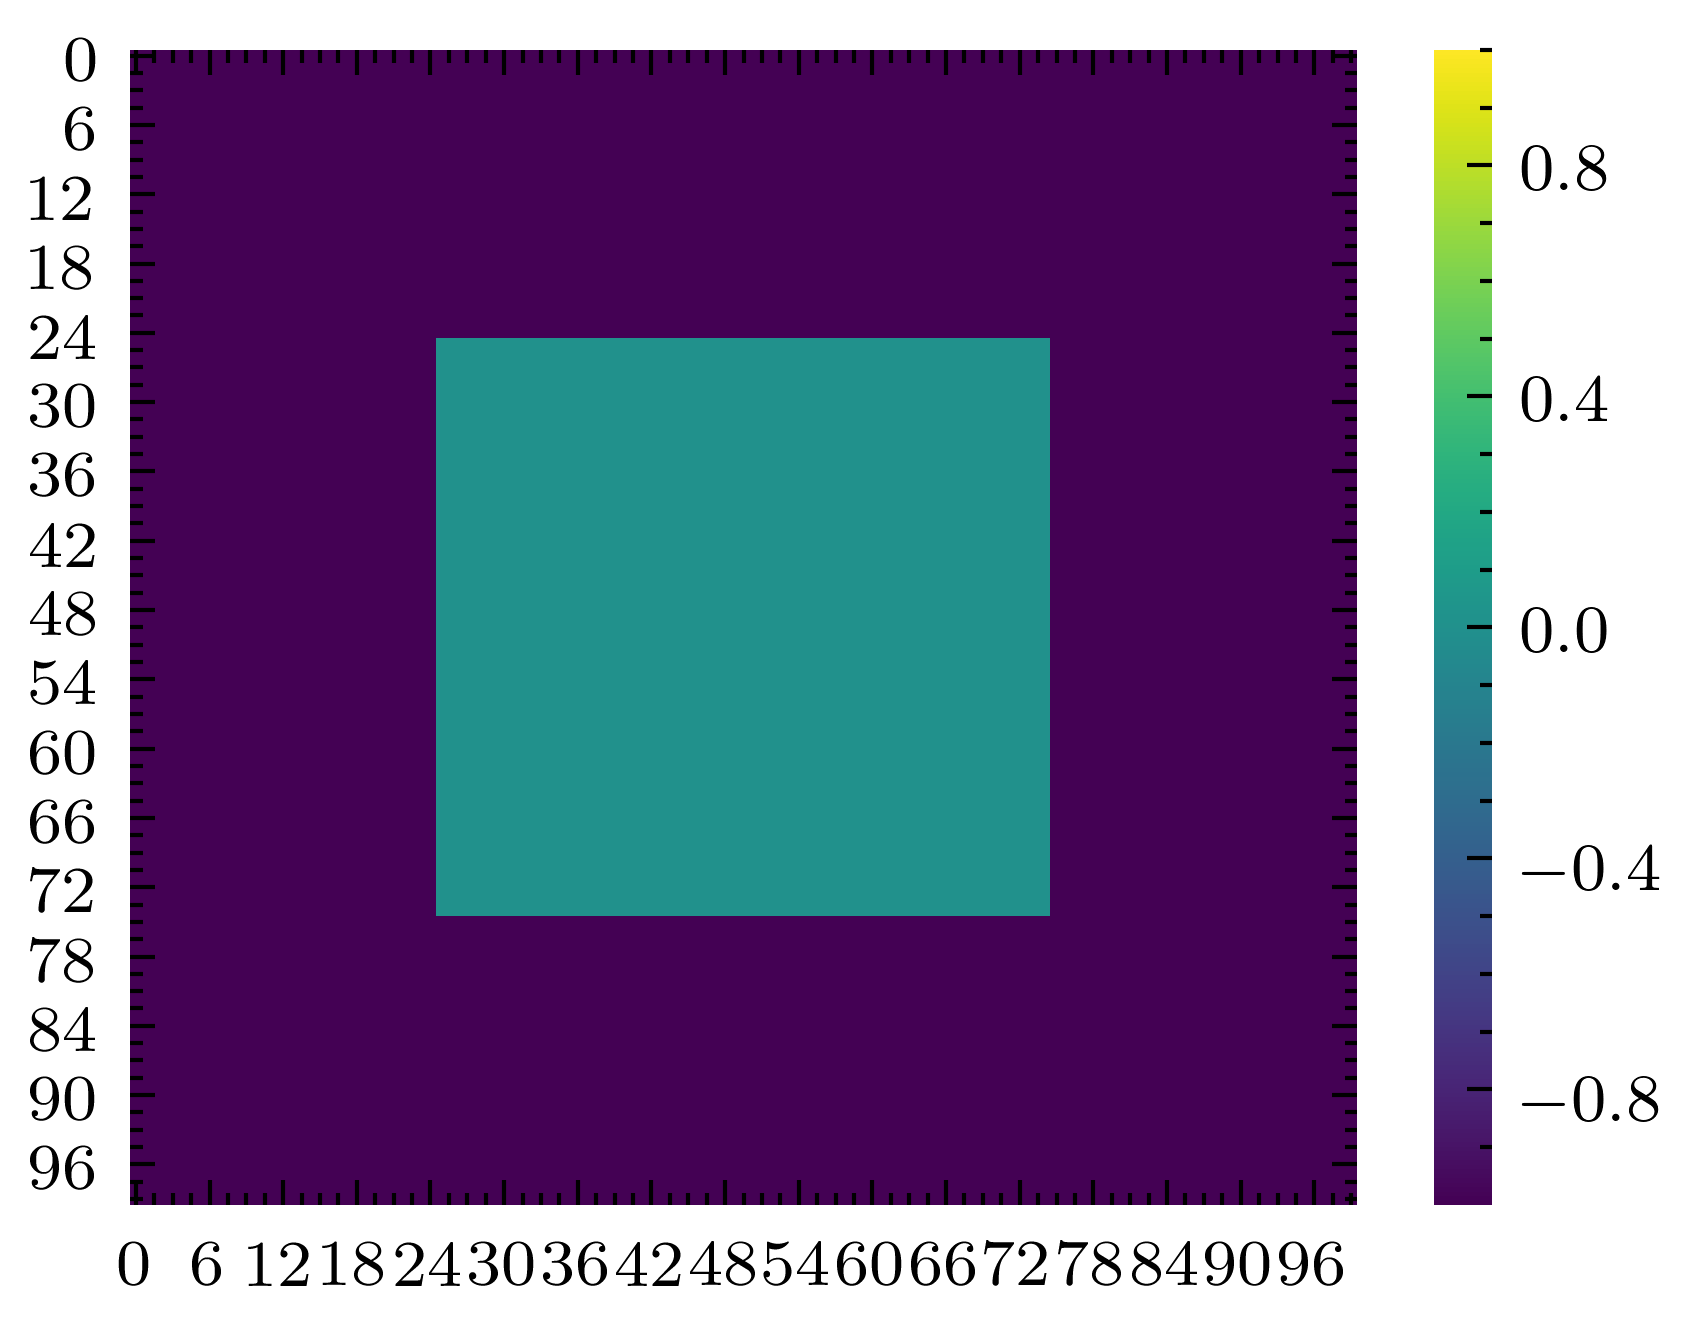
\includegraphics[width=\textwidth]{../img/data-aug/2d/square-middle-center.png}
        \caption{Height centered}
    \end{subfigure}  
    
          \begin{subfigure}[b]{0.5\textwidth}
        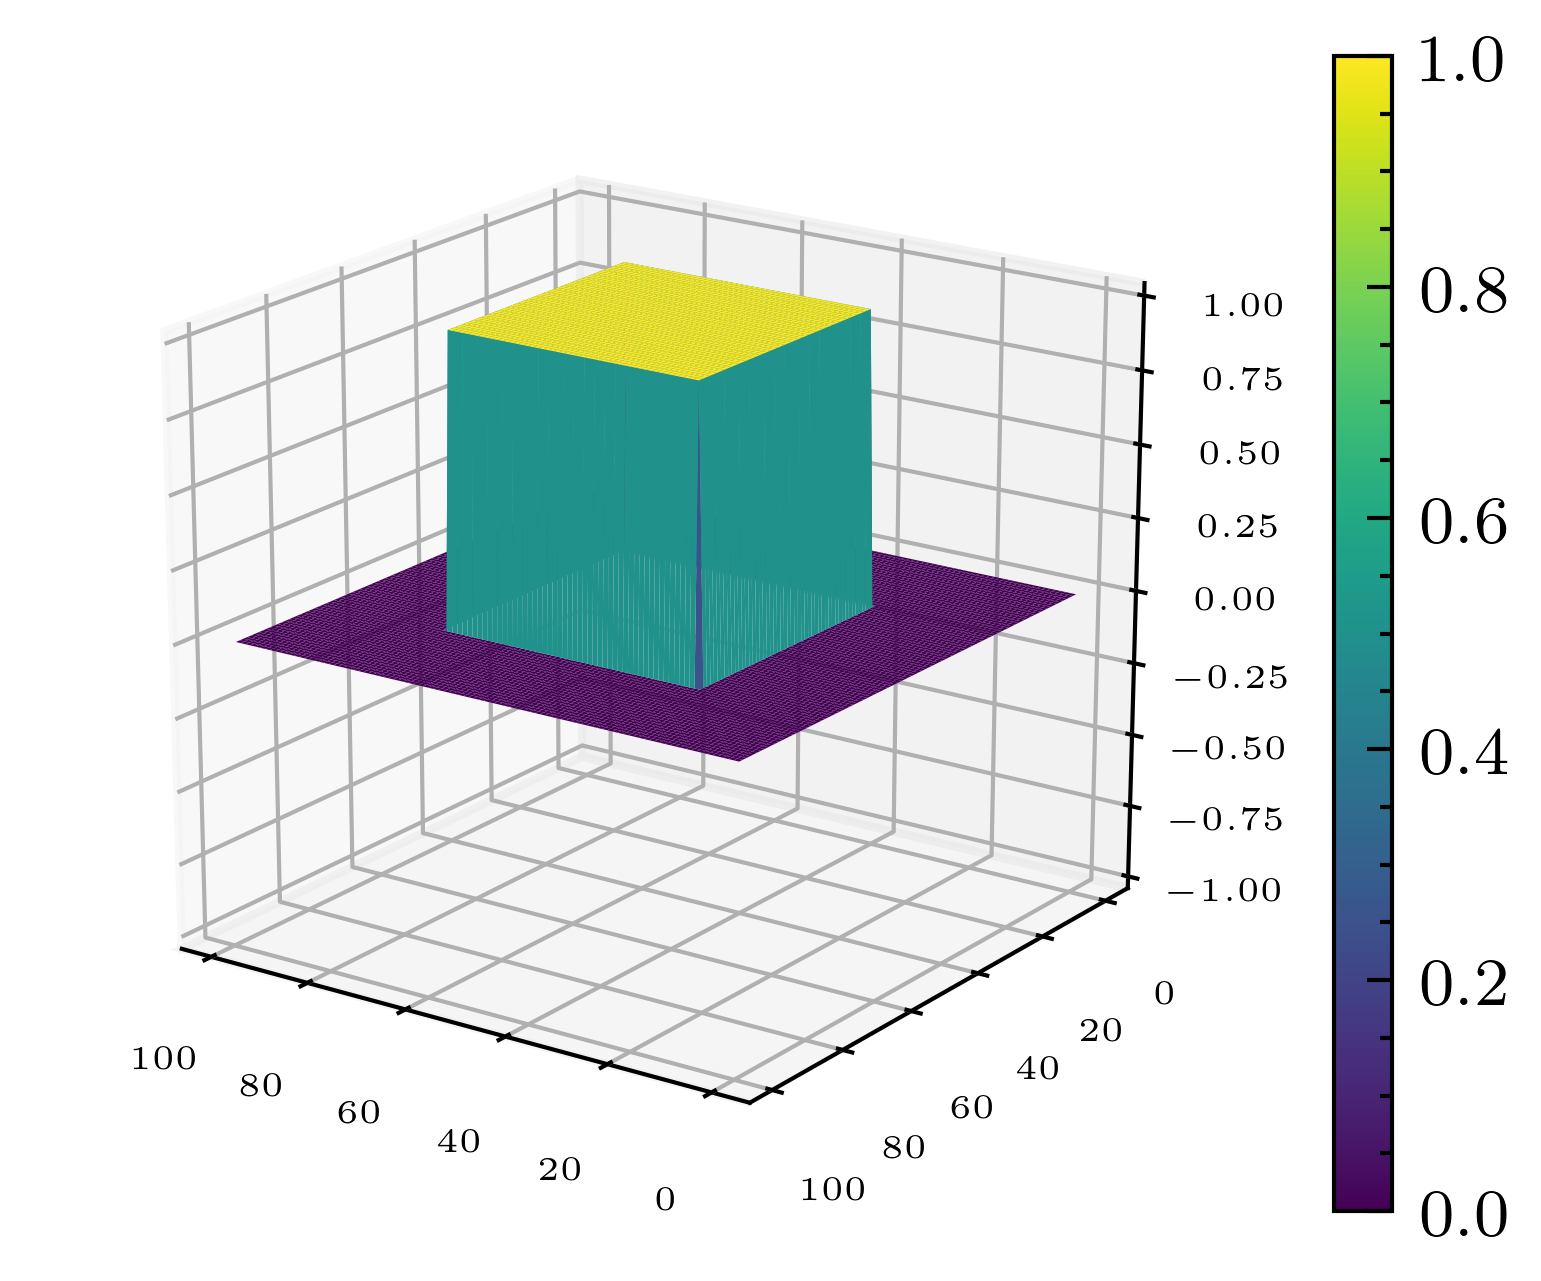
\includegraphics[width=\textwidth]{../img/data-aug/3d/square-middle.png}
        \caption{Input}
    \end{subfigure}
    \begin{subfigure}[b]{0.5\textwidth}
        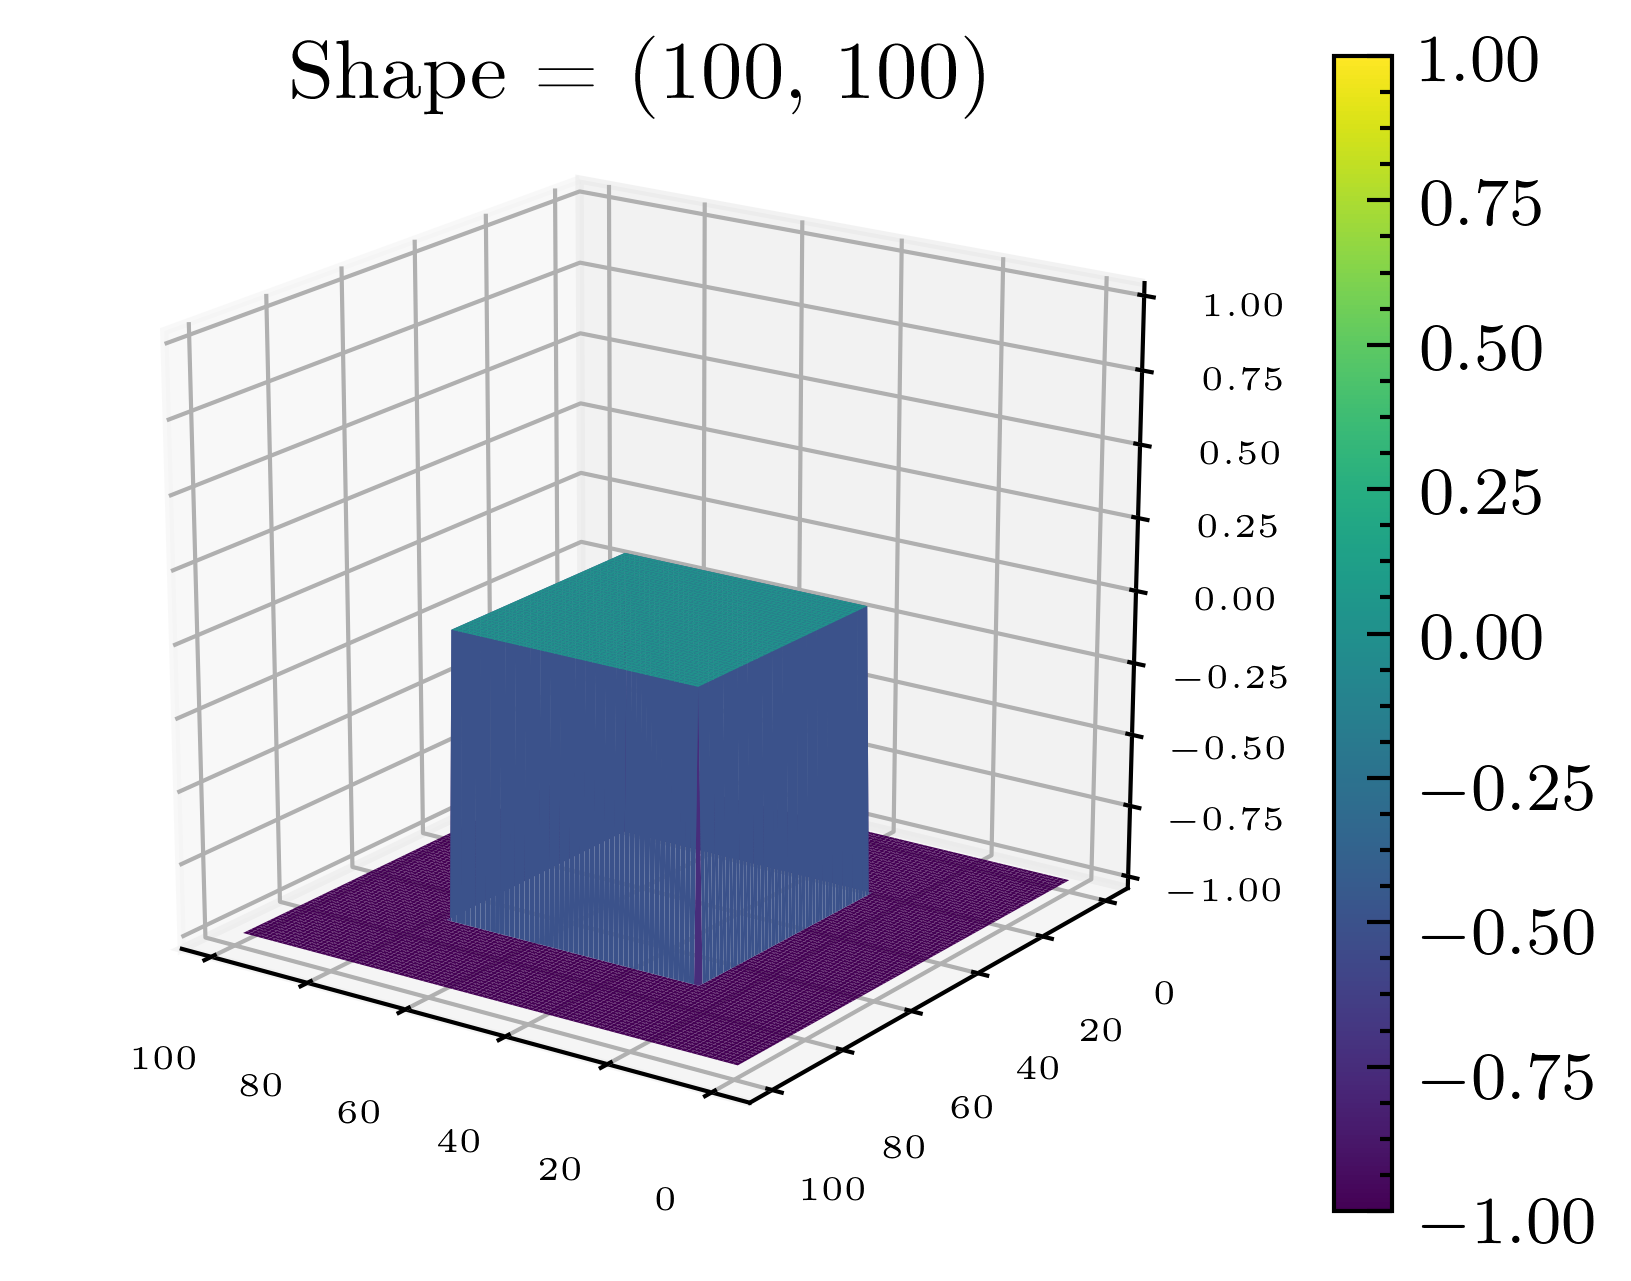
\includegraphics[width=\textwidth]{../img/data-aug/3d/square-middle-center.png}
        \caption{Height centered}
    \end{subfigure}  
\label{fig: center}
\caption{Normalization process}    
\end{figure}

\subsubsection{Data Augmentation}
\label{sec: data-aug}
Data augmentation is used to change the input of a model using different techniques to change it in order to produce more training examples. Since our inputs are heightmaps we cannot utilize the classic image manipulations such as shifts, flips, and zooms. Imagine that we have a patch with a wall in front of it, if we random rotate the image the wall may go in a position where the patch it is now traversable but its label is still not traversable, we have to be more creative. We decided to apply dropout, coarse dropout, and random simplex noise since they are traversability invariant. To illustrate those techniques we are going to use the following example patch of size $100x100$.
\begin{figure}[H]
    \begin{subfigure}[b]{0.5\textwidth}
        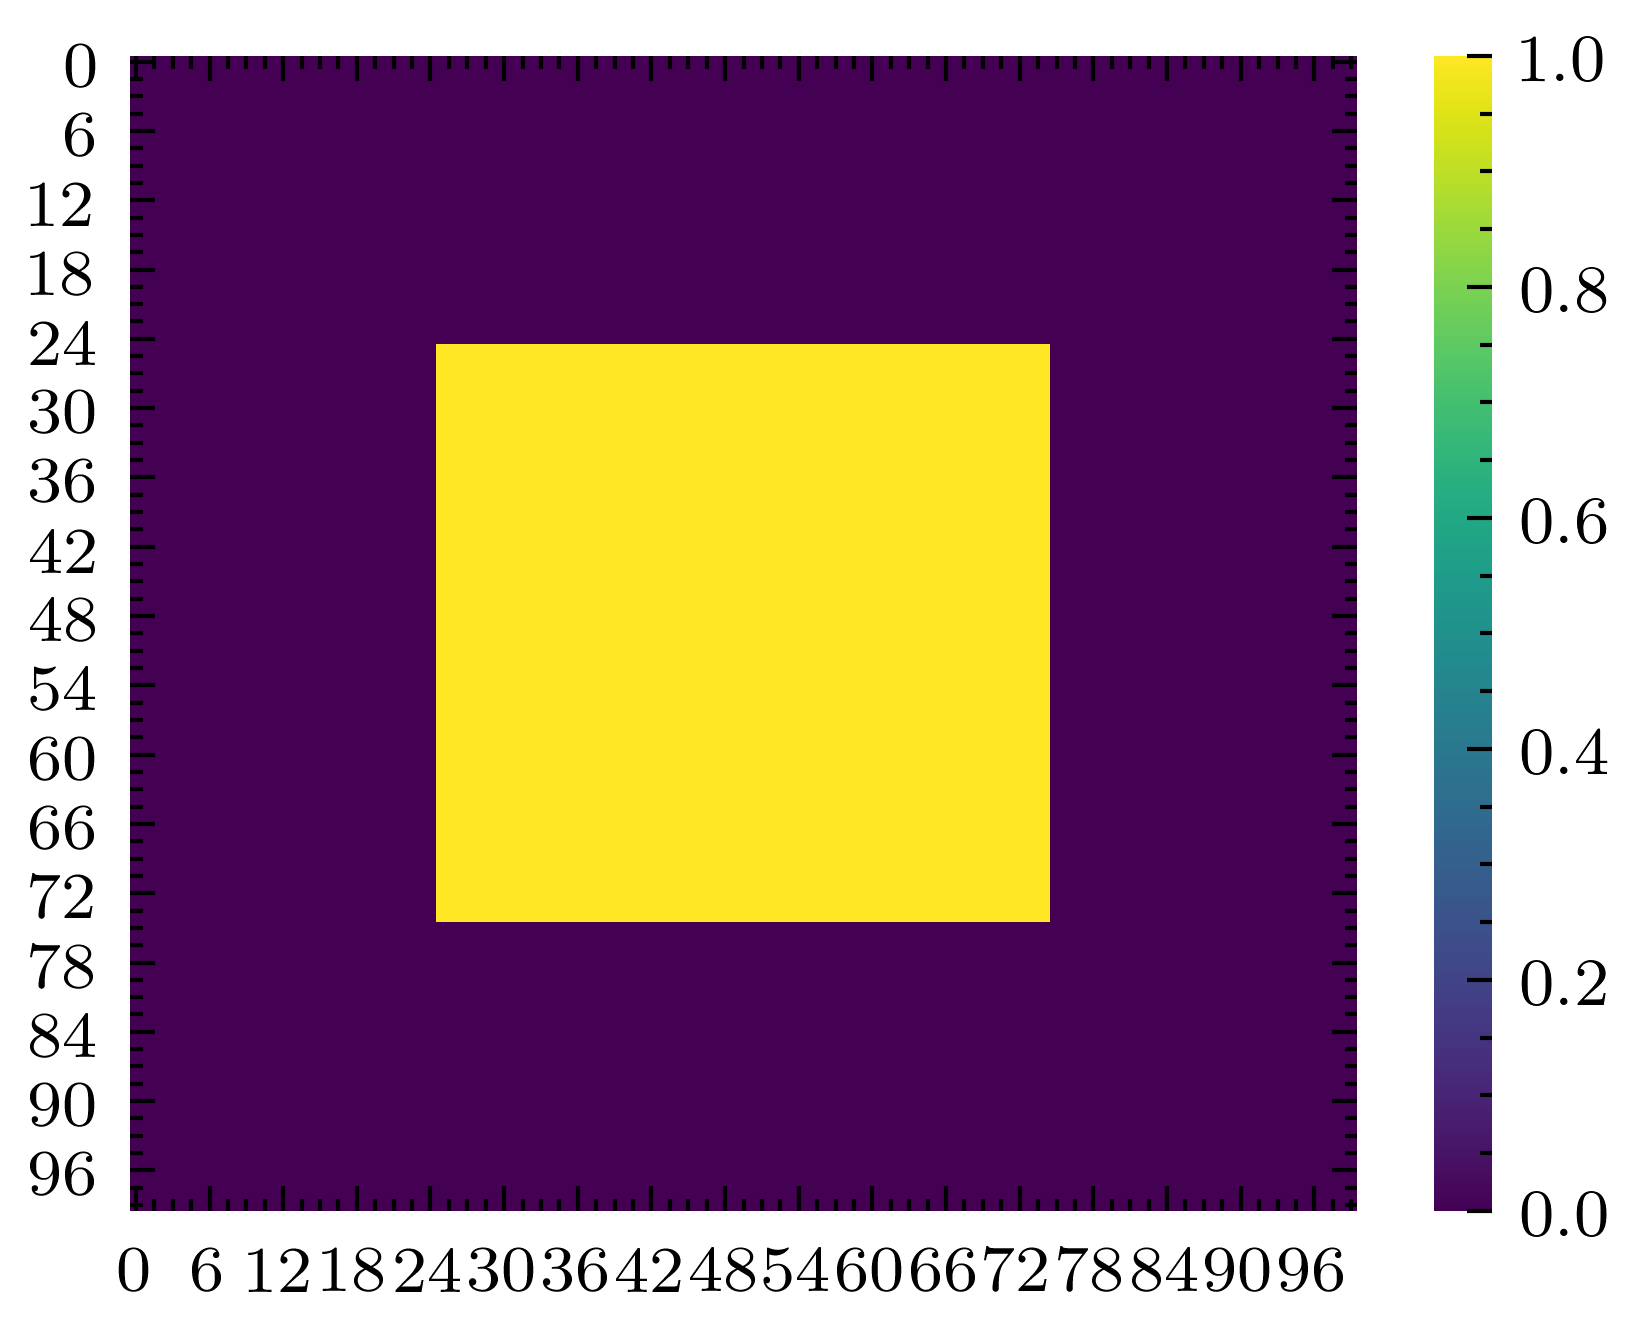
\includegraphics[width=\textwidth]{../img/data-aug/2d/square-middle.png}
    \end{subfigure}
    \begin{subfigure}[b]{0.5\textwidth}
        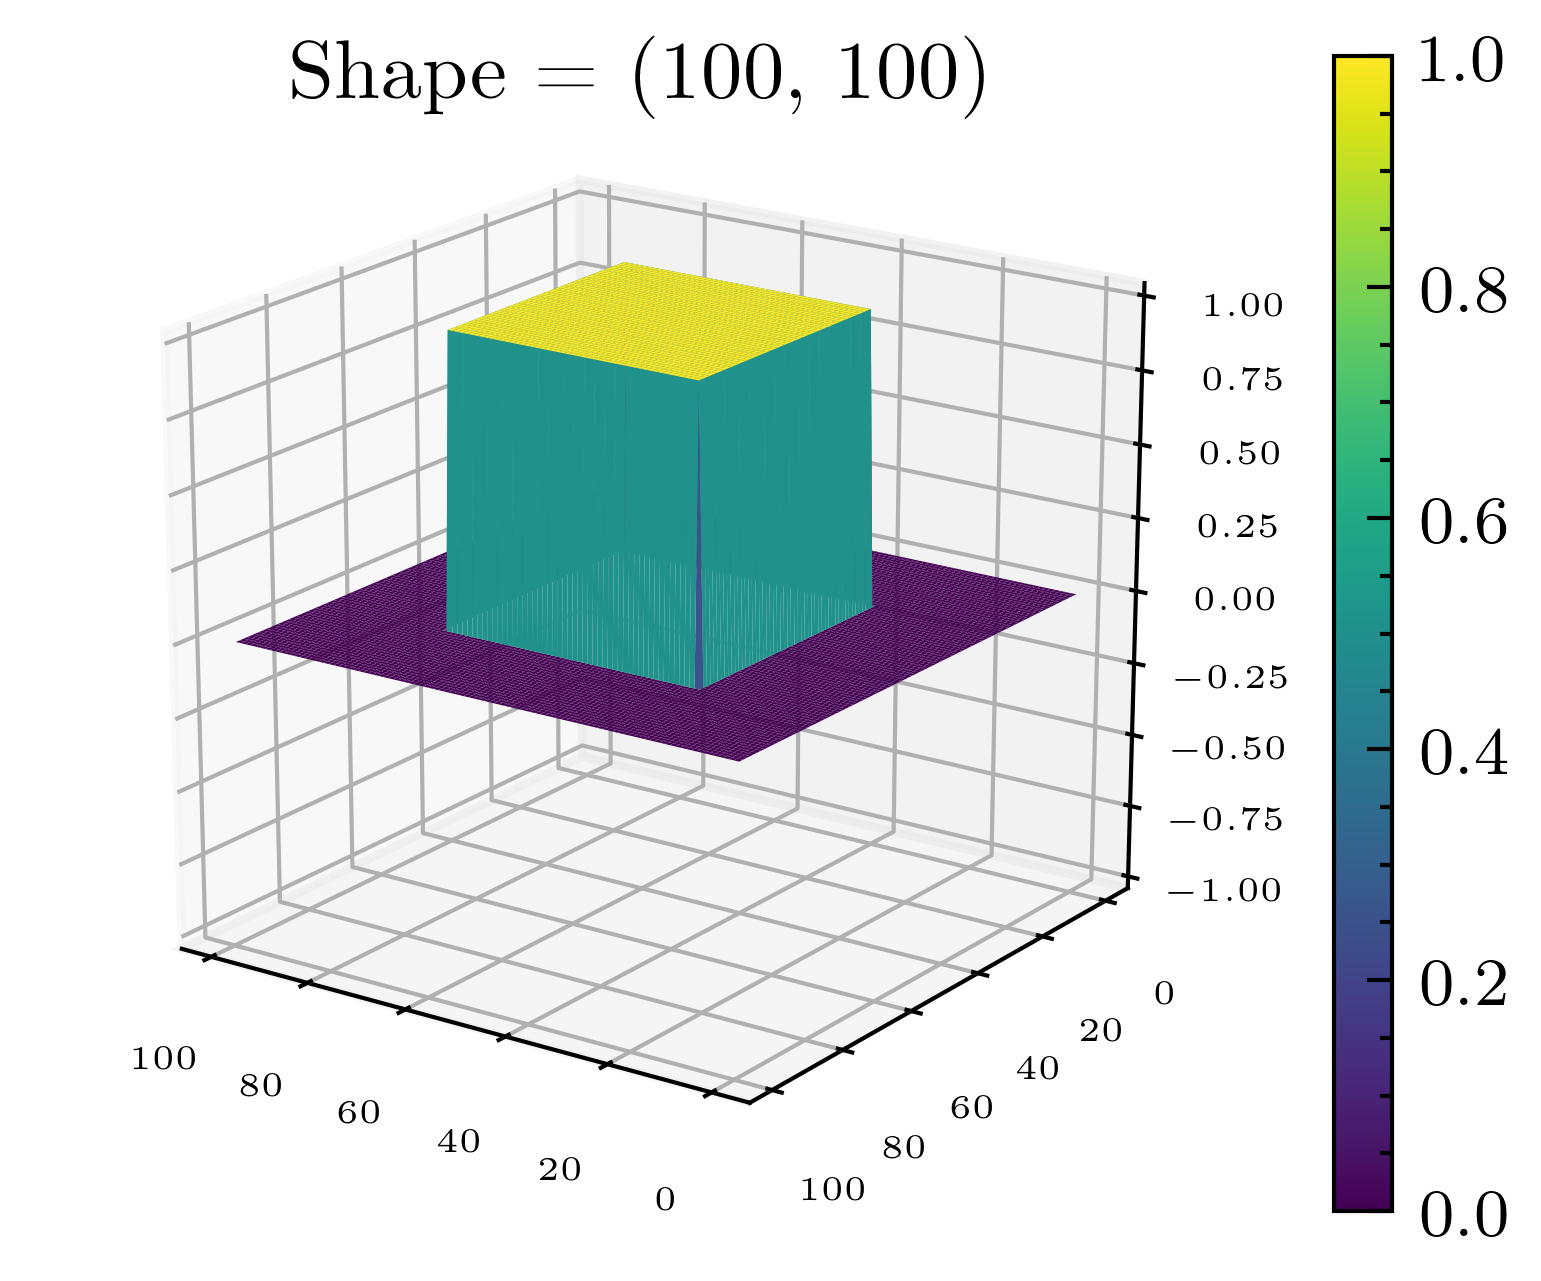
\includegraphics[width=\textwidth]{../img/data-aug/square-middle.png}
    \end{subfigure}    
\label{fig: square-patch}
\caption{A patch with a square in the middle}    
\end{figure}
\paragraph{Dropout} is a technique to randomly set some pixels to zero, in our case we flat some random pixel in the patch. 
\paragraph{Coarse Dropout} similar to dropout, it sets to zero random regions of pixels.
\paragraph{Simplex Noise} is a form of Perlin noise that is mostly used in ground generation. Our idea is to add some noise to make the network generalize better since lots of training maps have only obstacles in flat ground. Since it is computationally expensive, we randomly fist apply the noise to five hundred images with only zeros. Then, we randomly scaled them and add to the input image.
\begin{figure}[H]
    \centering

        \begin{subfigure}[b]{0.45\textwidth}
            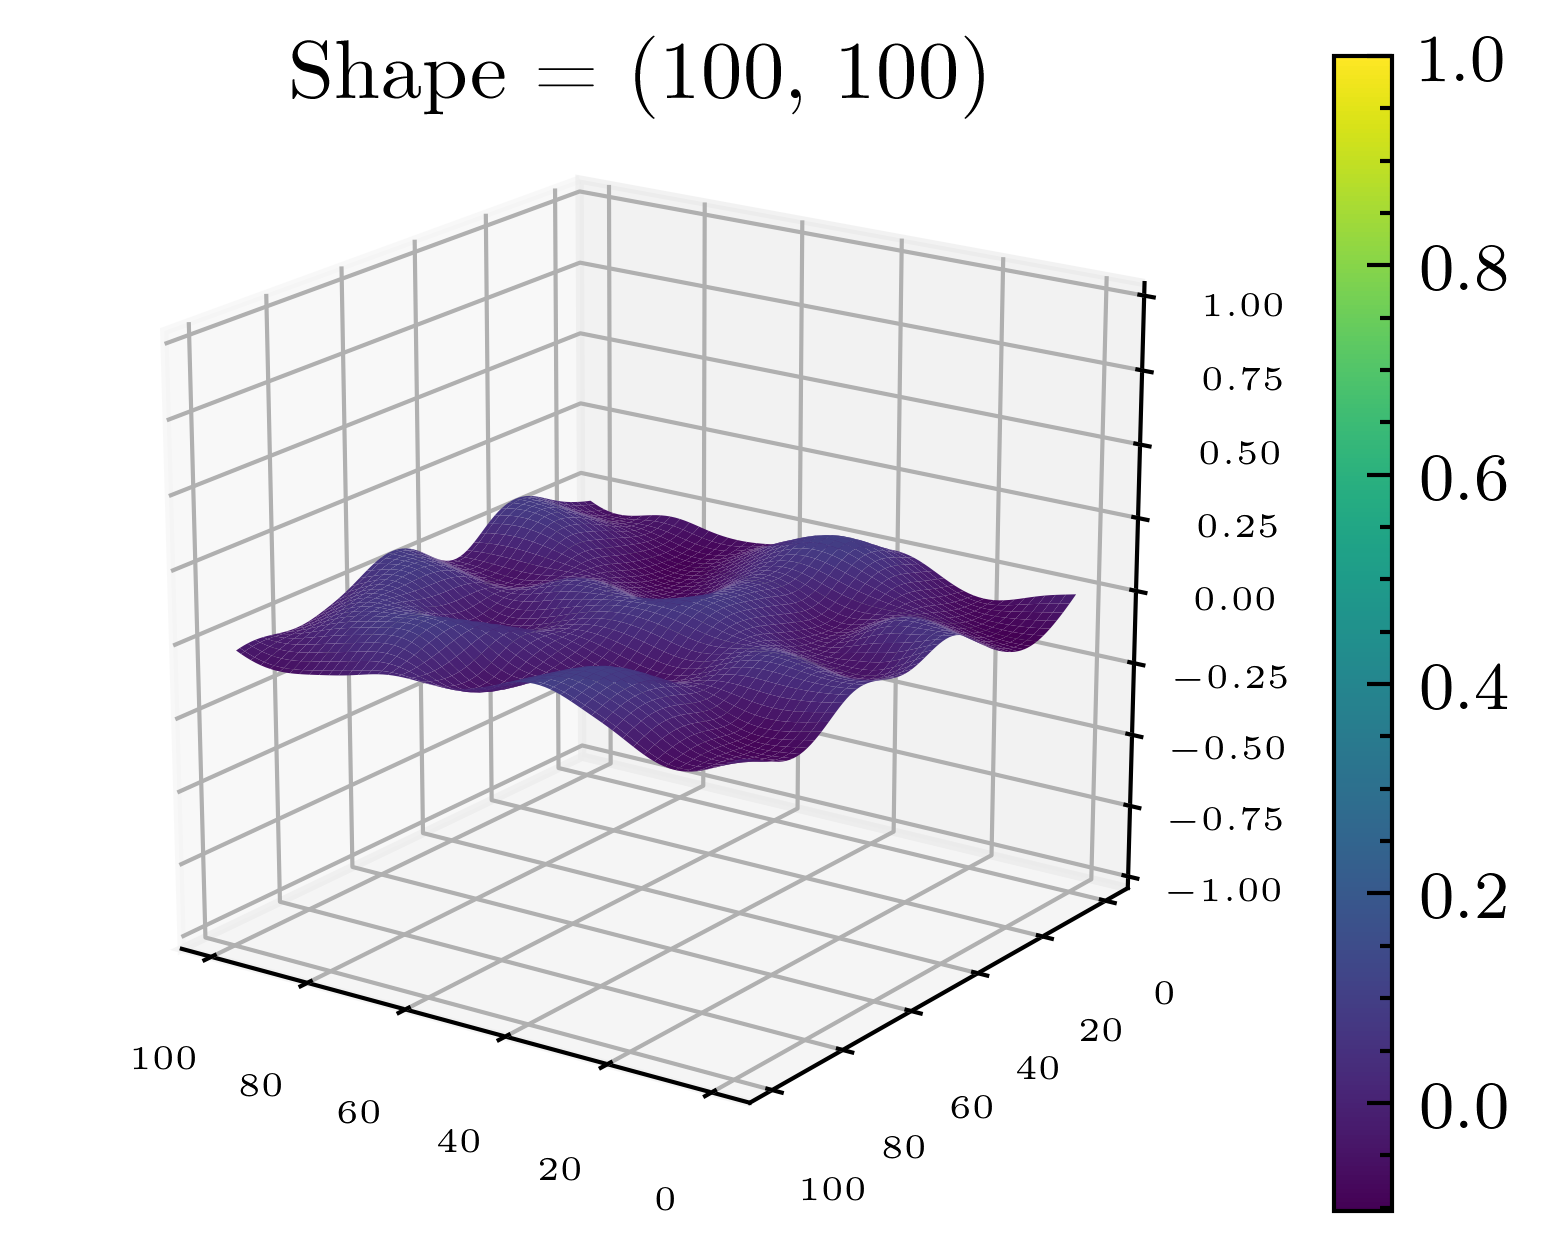
\includegraphics[width=\textwidth]{../img/data-aug/3d/simplex1.png}
            \caption{Features size = 10}
        \end{subfigure}
        \begin{subfigure}[b]{0.45\linewidth}
            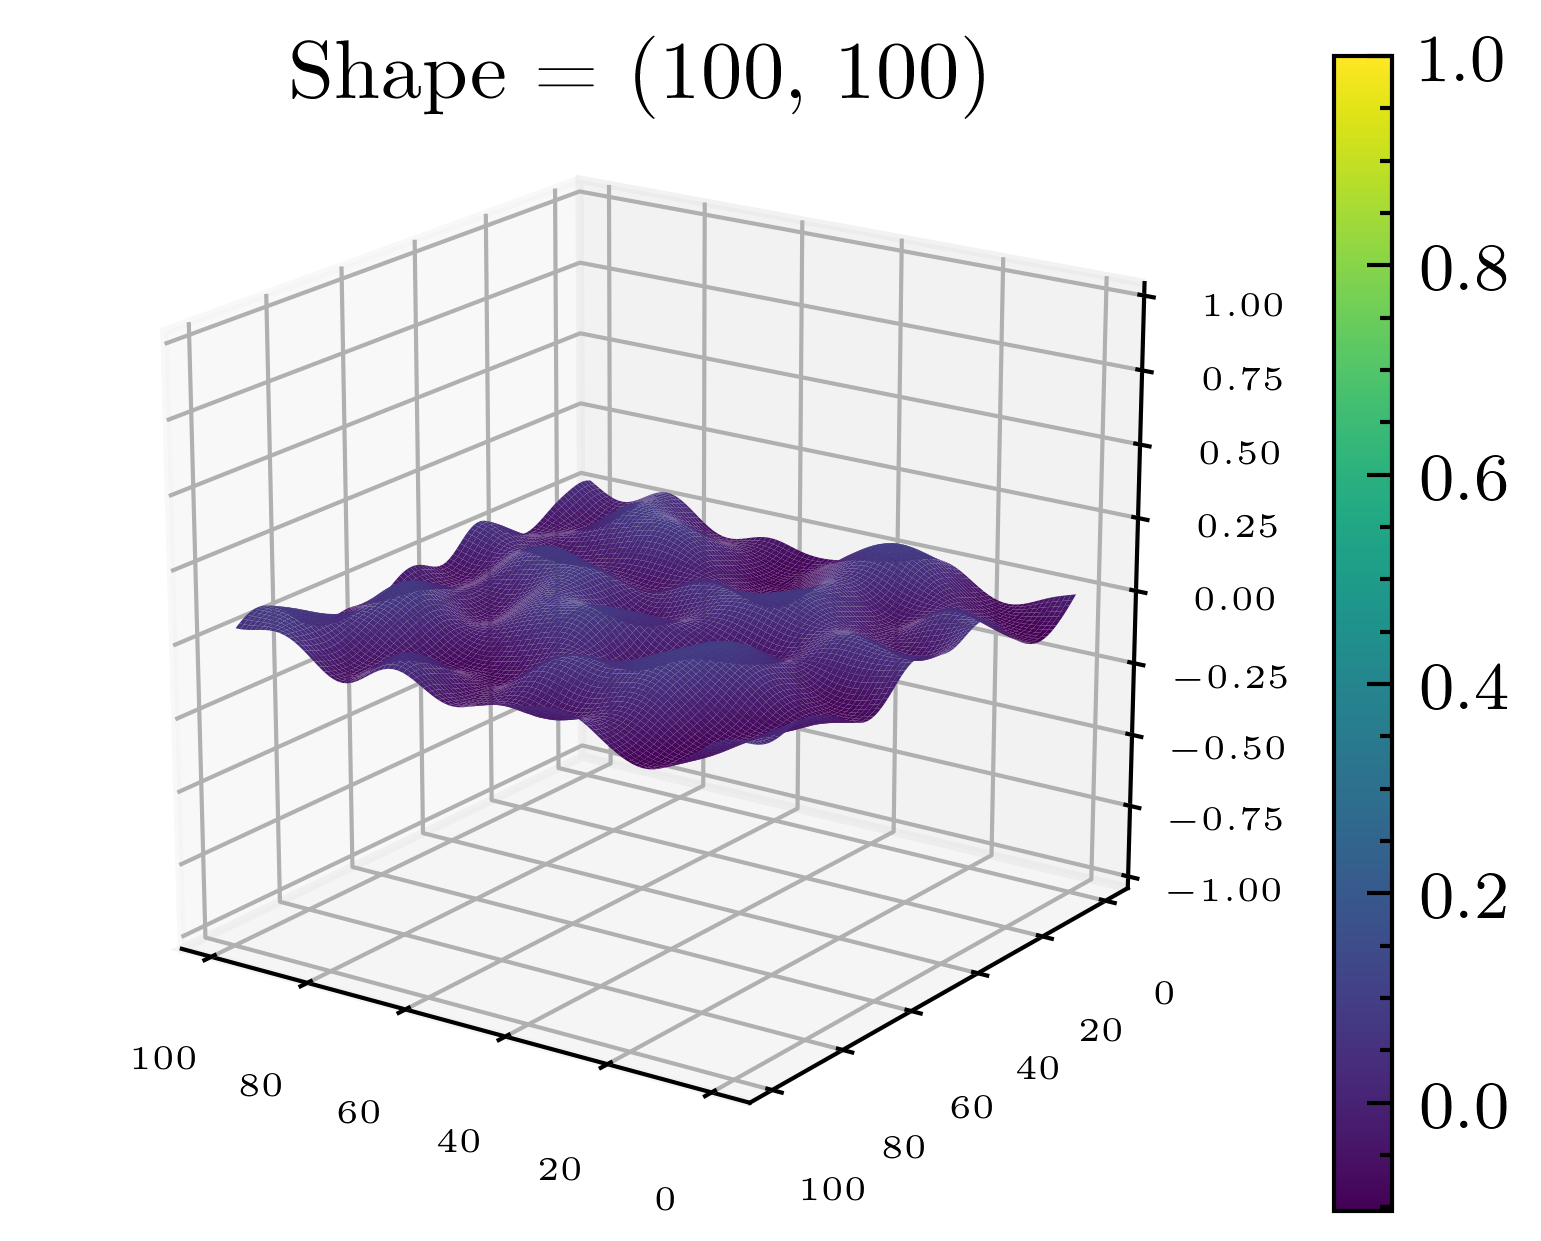
\includegraphics[width=\textwidth]{../img/data-aug/3d/simplex2.png}
            \caption{Data-aug}
            \end{subfigure}    
          \begin{subfigure}[b]{0.45\textwidth}
            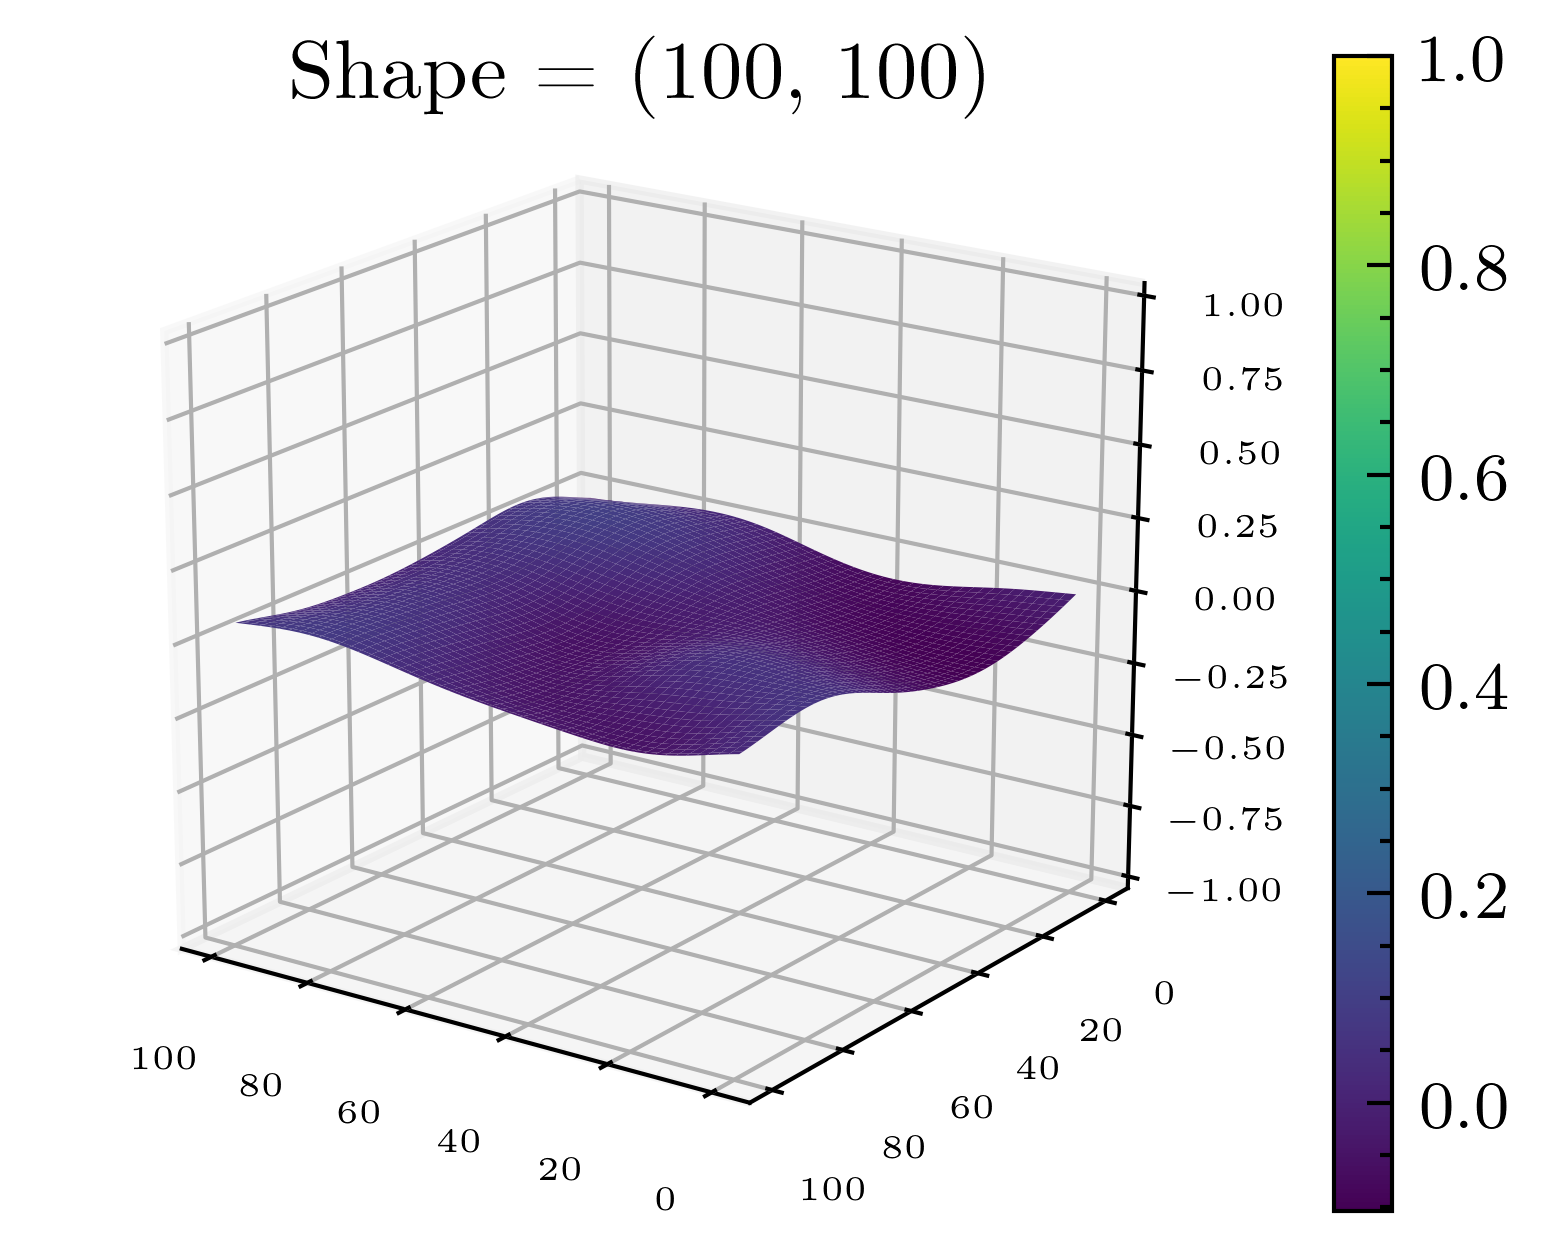
\includegraphics[width=\textwidth]{../img/data-aug/3d/simplex3.png}
            \caption{Features size = 30}
        \end{subfigure}    
        \begin{subfigure}[b]{0.45\textwidth}
            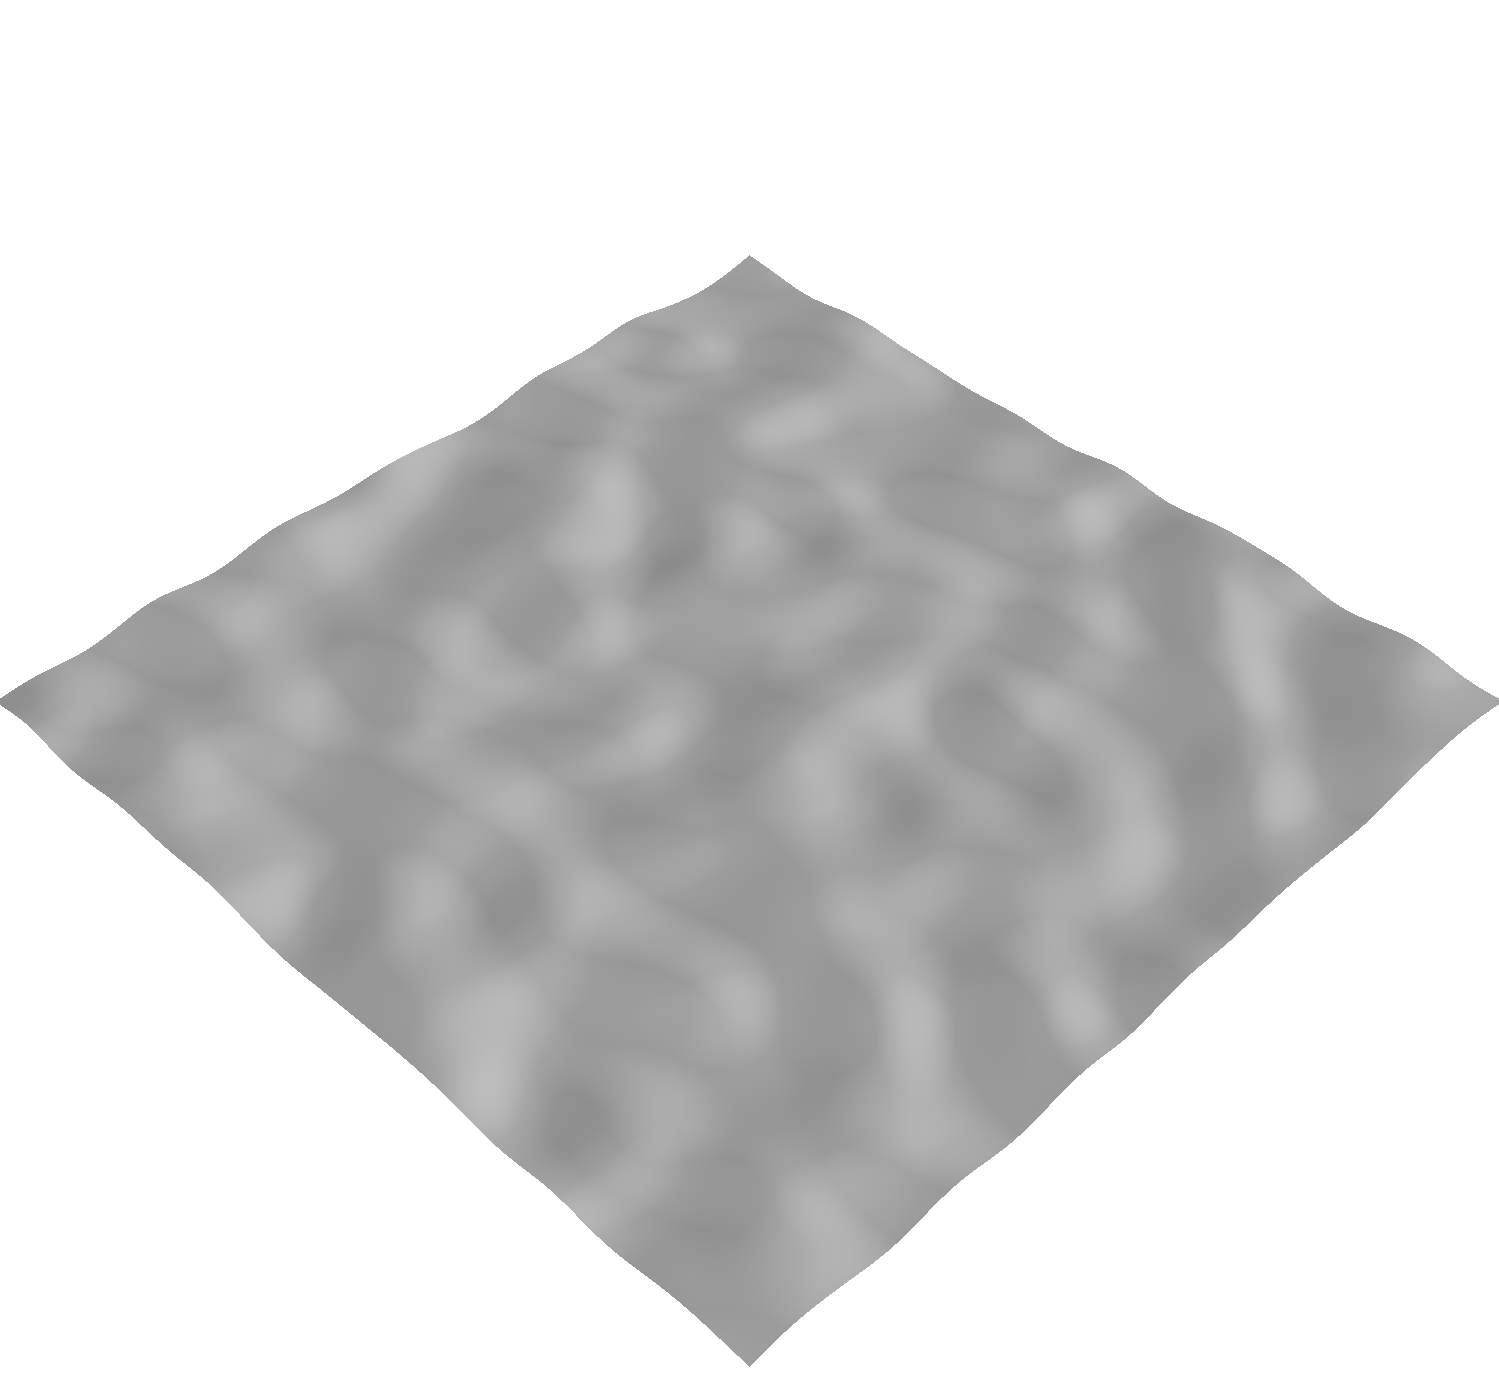
\includegraphics[width=\textwidth]{../img/data-aug/3d/simplex4.png}
            \caption{Features size = 40}
        \end{subfigure}    
    \label{fig: simplex-noise}
    \caption{Simplex Noise on flat ground}    
\end{figure}

The following images show the tree data augmentation techniques used applied the input image.
\begin{figure}[H]
    \centering
        \begin{subfigure}[b]{0.45\textwidth}
            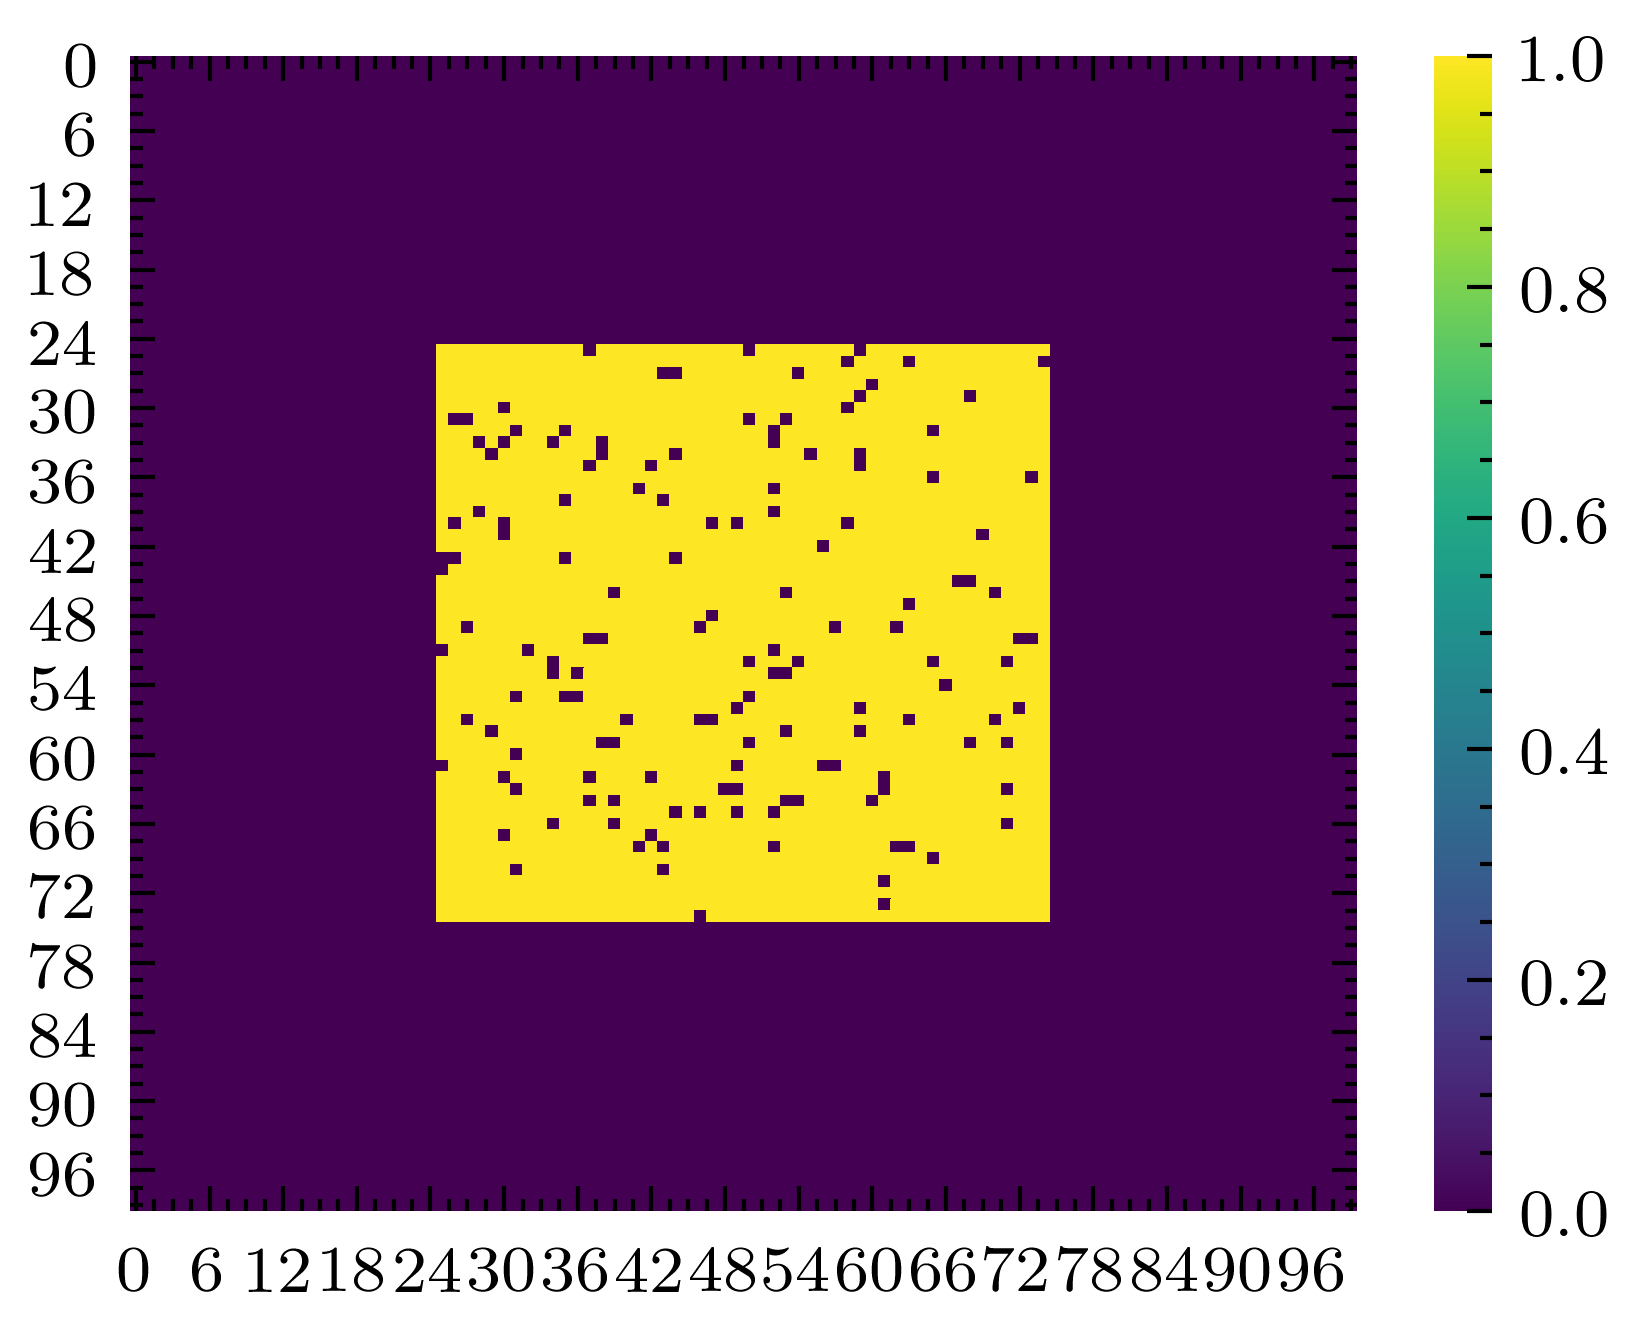
\includegraphics[width=\textwidth]{../img/data-aug/2d/center-dropout.png}
            \caption{Dropout}
        \end{subfigure}
        \begin{subfigure}[b]{0.45\linewidth}
            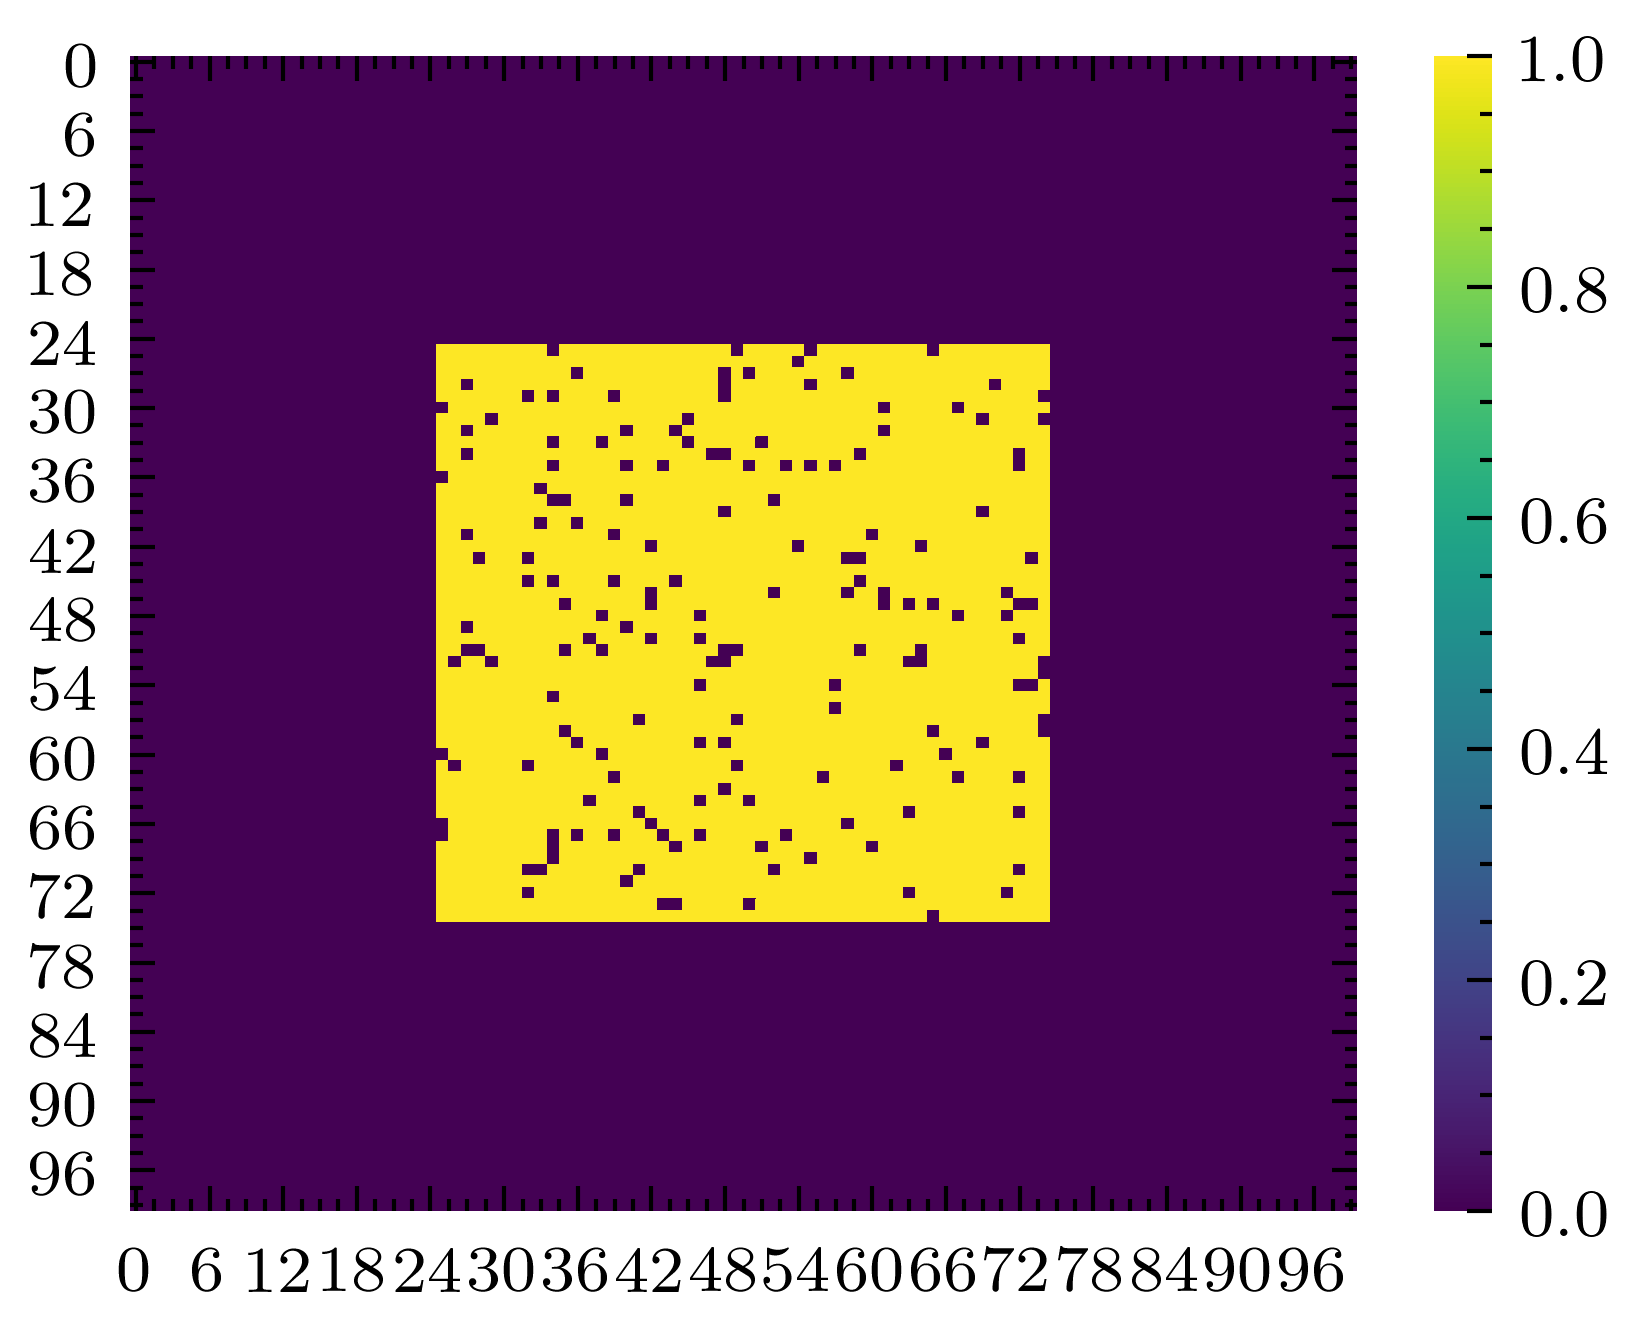
\includegraphics[width=\textwidth]{../img/data-aug/2d/center-coarse-dropout.png}
            \caption{Coarse Dropout}
            \end{subfigure}    

          \begin{subfigure}[b]{0.45\textwidth}
            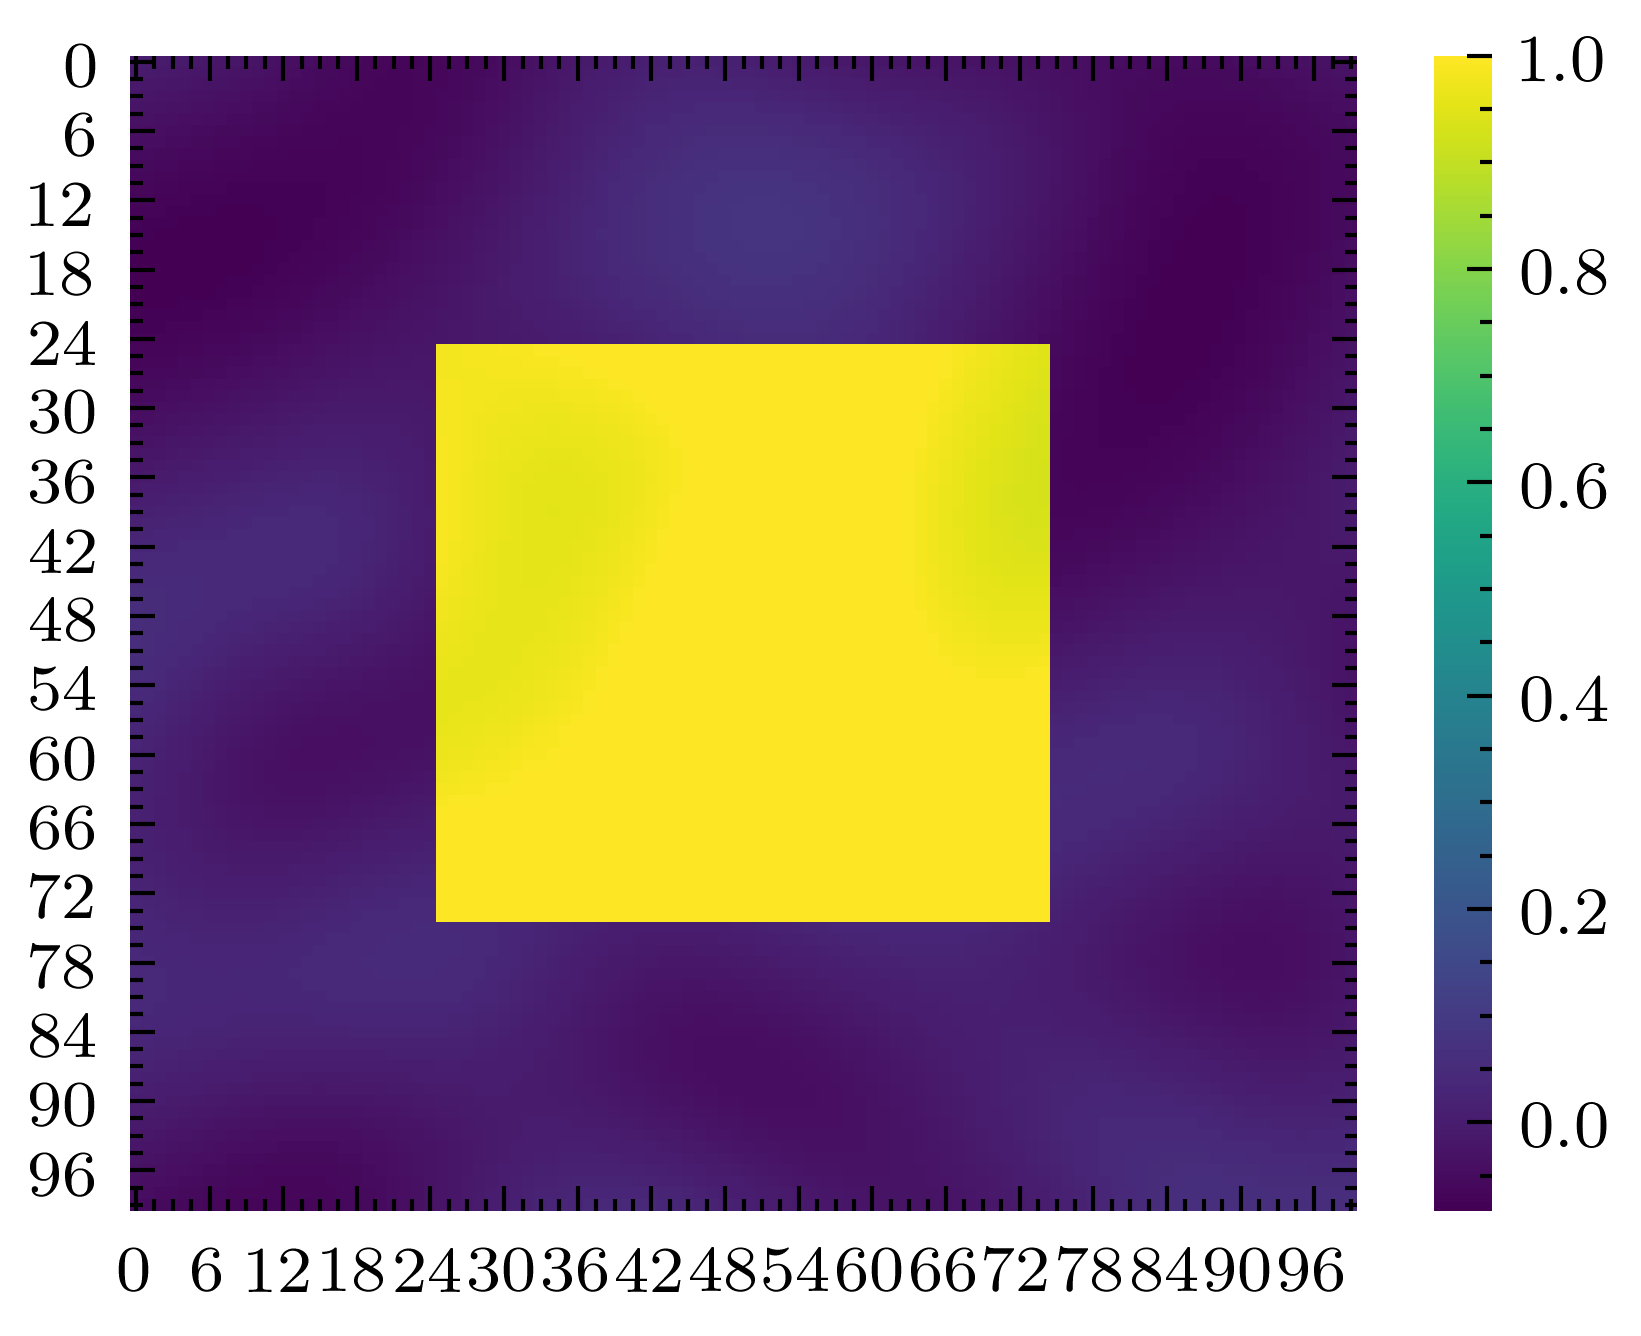
\includegraphics[width=\textwidth]{../img/data-aug/2d/center-simplex.png}
            \caption{Simplex Noise}

        \end{subfigure}    
        \begin{subfigure}[b]{0.45\textwidth}
            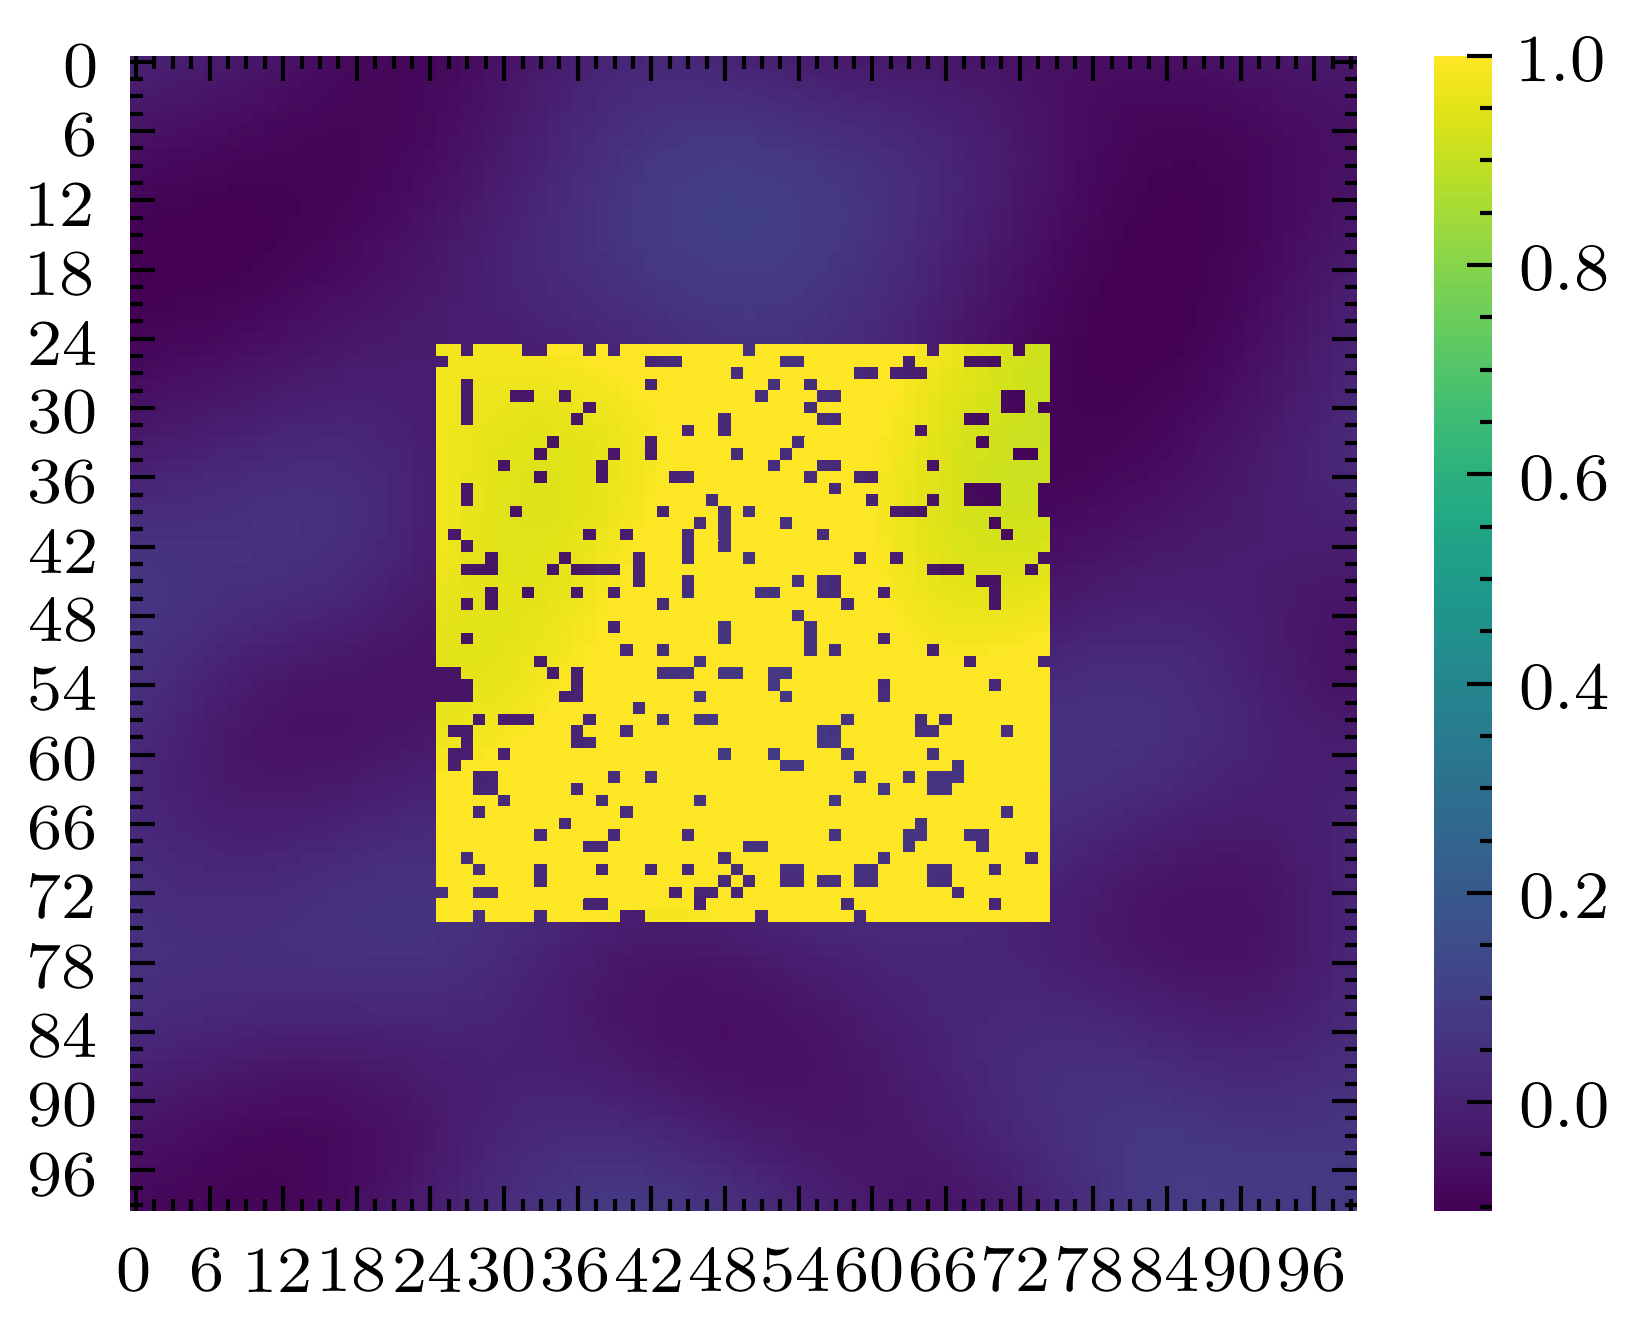
\includegraphics[width=\textwidth]{../img/data-aug/2d/center-aug.png}
            \caption{Final result}
        \end{subfigure}    
    \label{fig: square-patch-aug}
    \caption{Data augmentation}    
\end{figure}
It follows an other set of figures that shows the data augmentation we utilised on different inputs.

\begin{figure}[H]
    \centering
        \begin{subfigure}[b]{0.45\textwidth}
            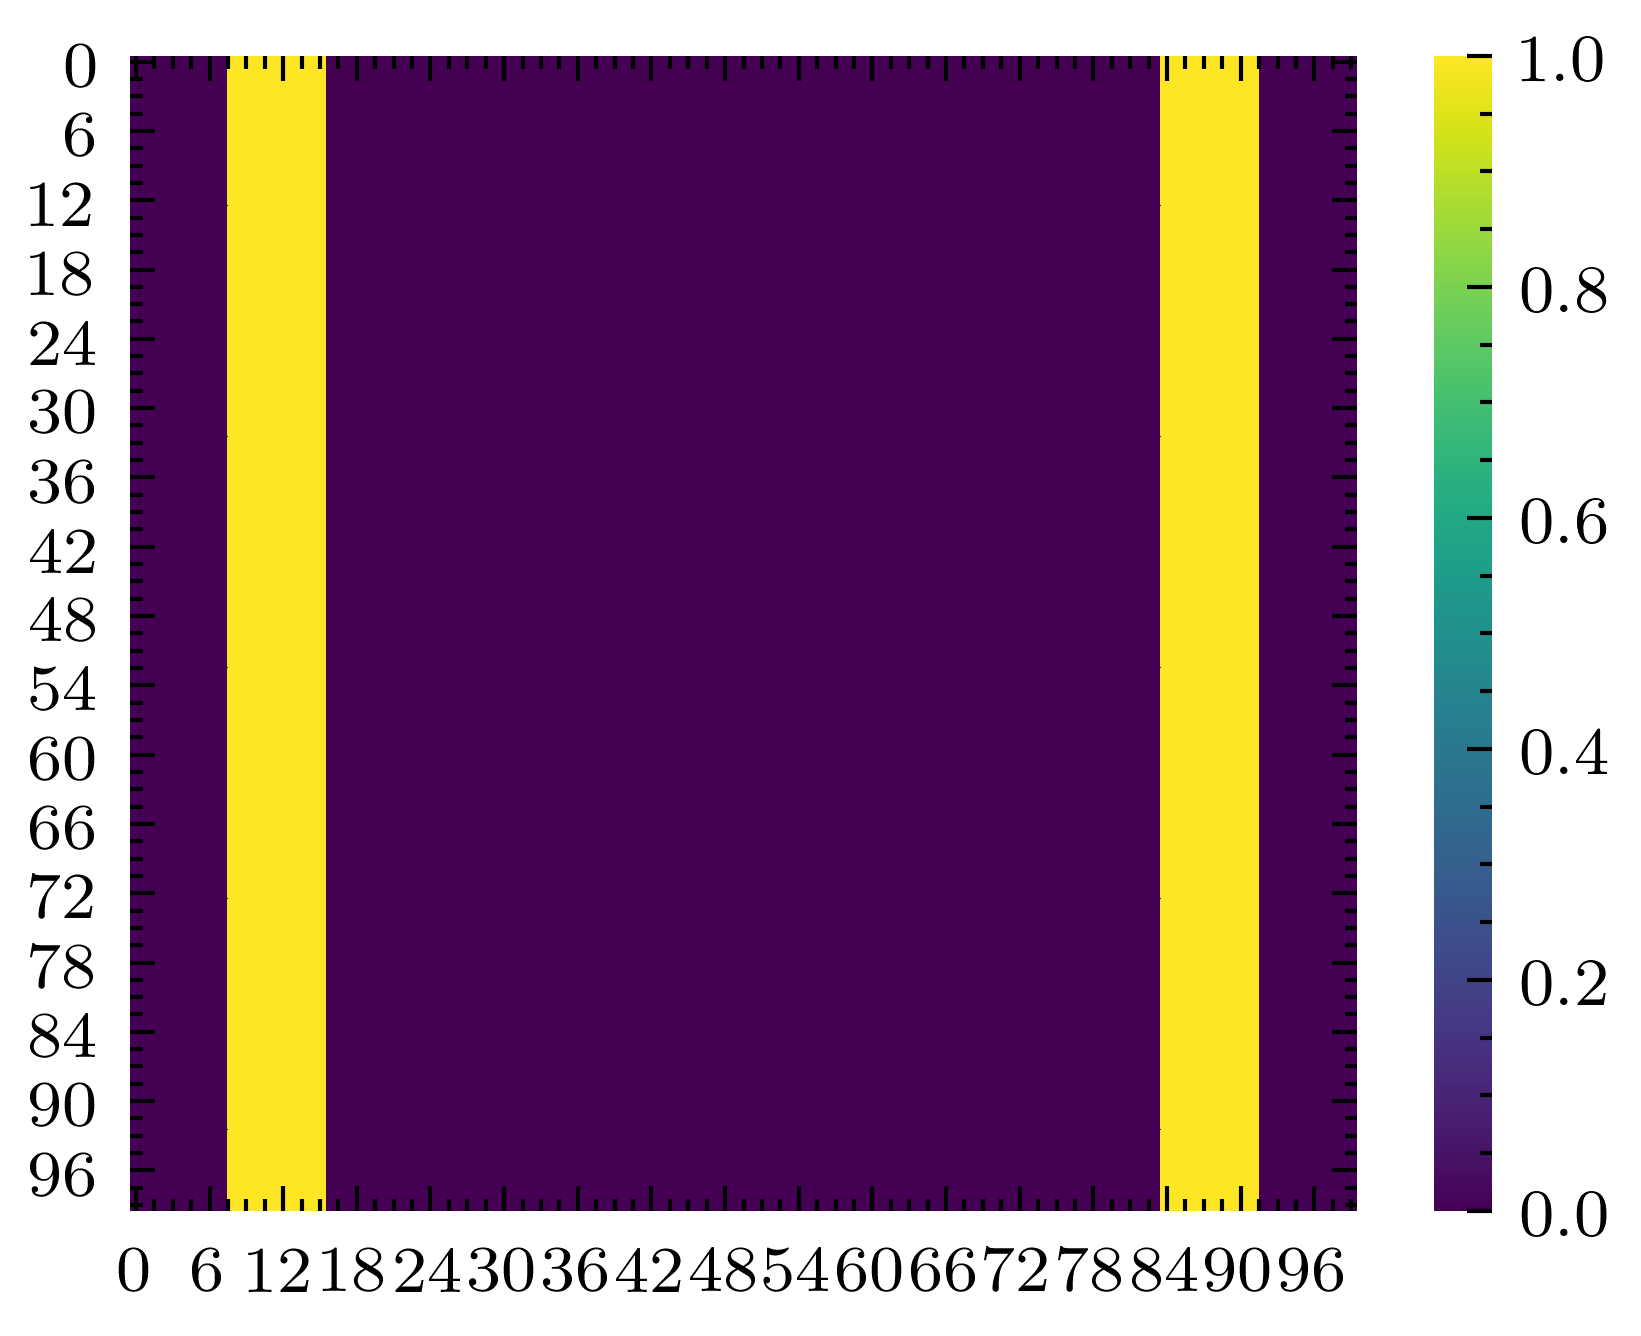
\includegraphics[width=\textwidth]{../img/data-aug/2d/wall.png}
            \caption{Walls}
        \end{subfigure}
        \begin{subfigure}[b]{0.45\linewidth}
            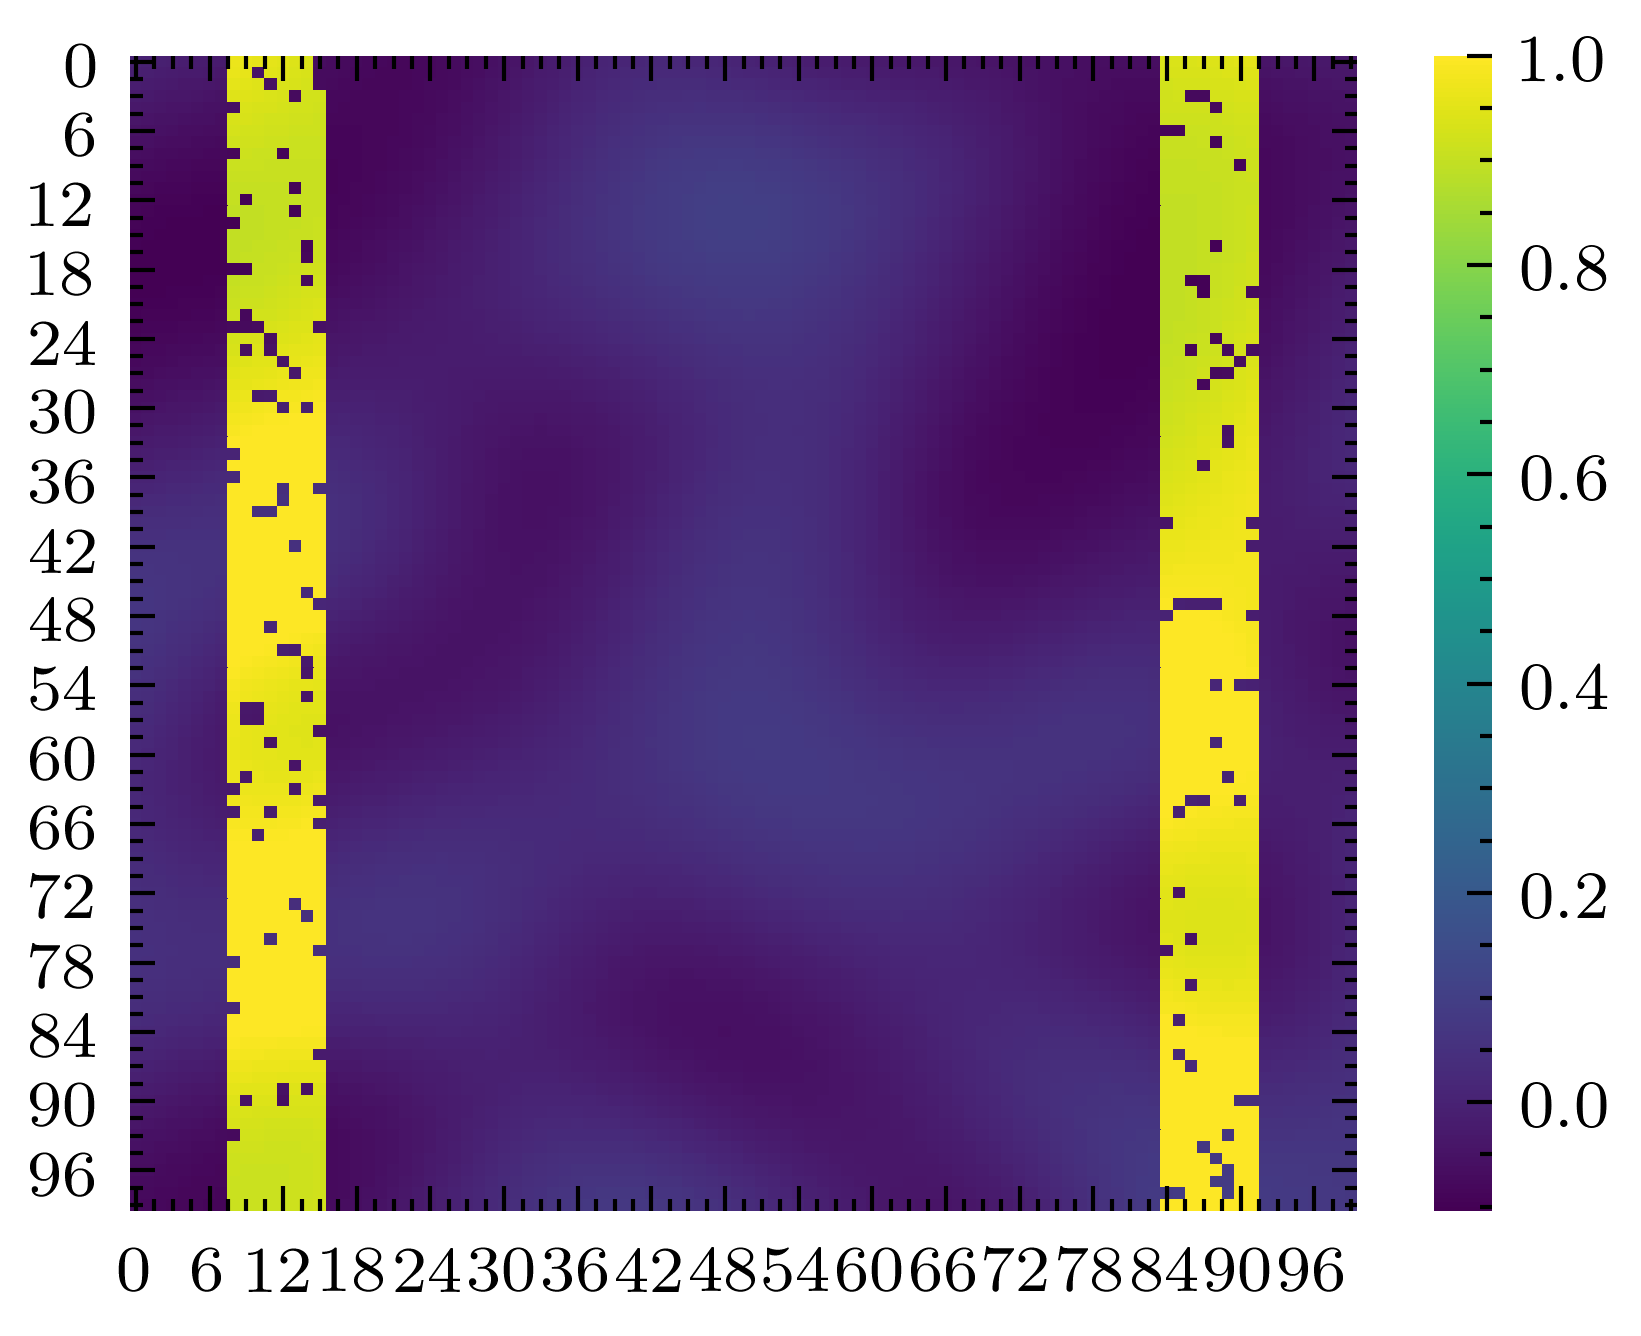
\includegraphics[width=\textwidth]{../img/data-aug/2d/wall-aug.png}
            \caption{Walls aug}
        \end{subfigure}    
        \begin{subfigure}[b]{0.45\textwidth}
            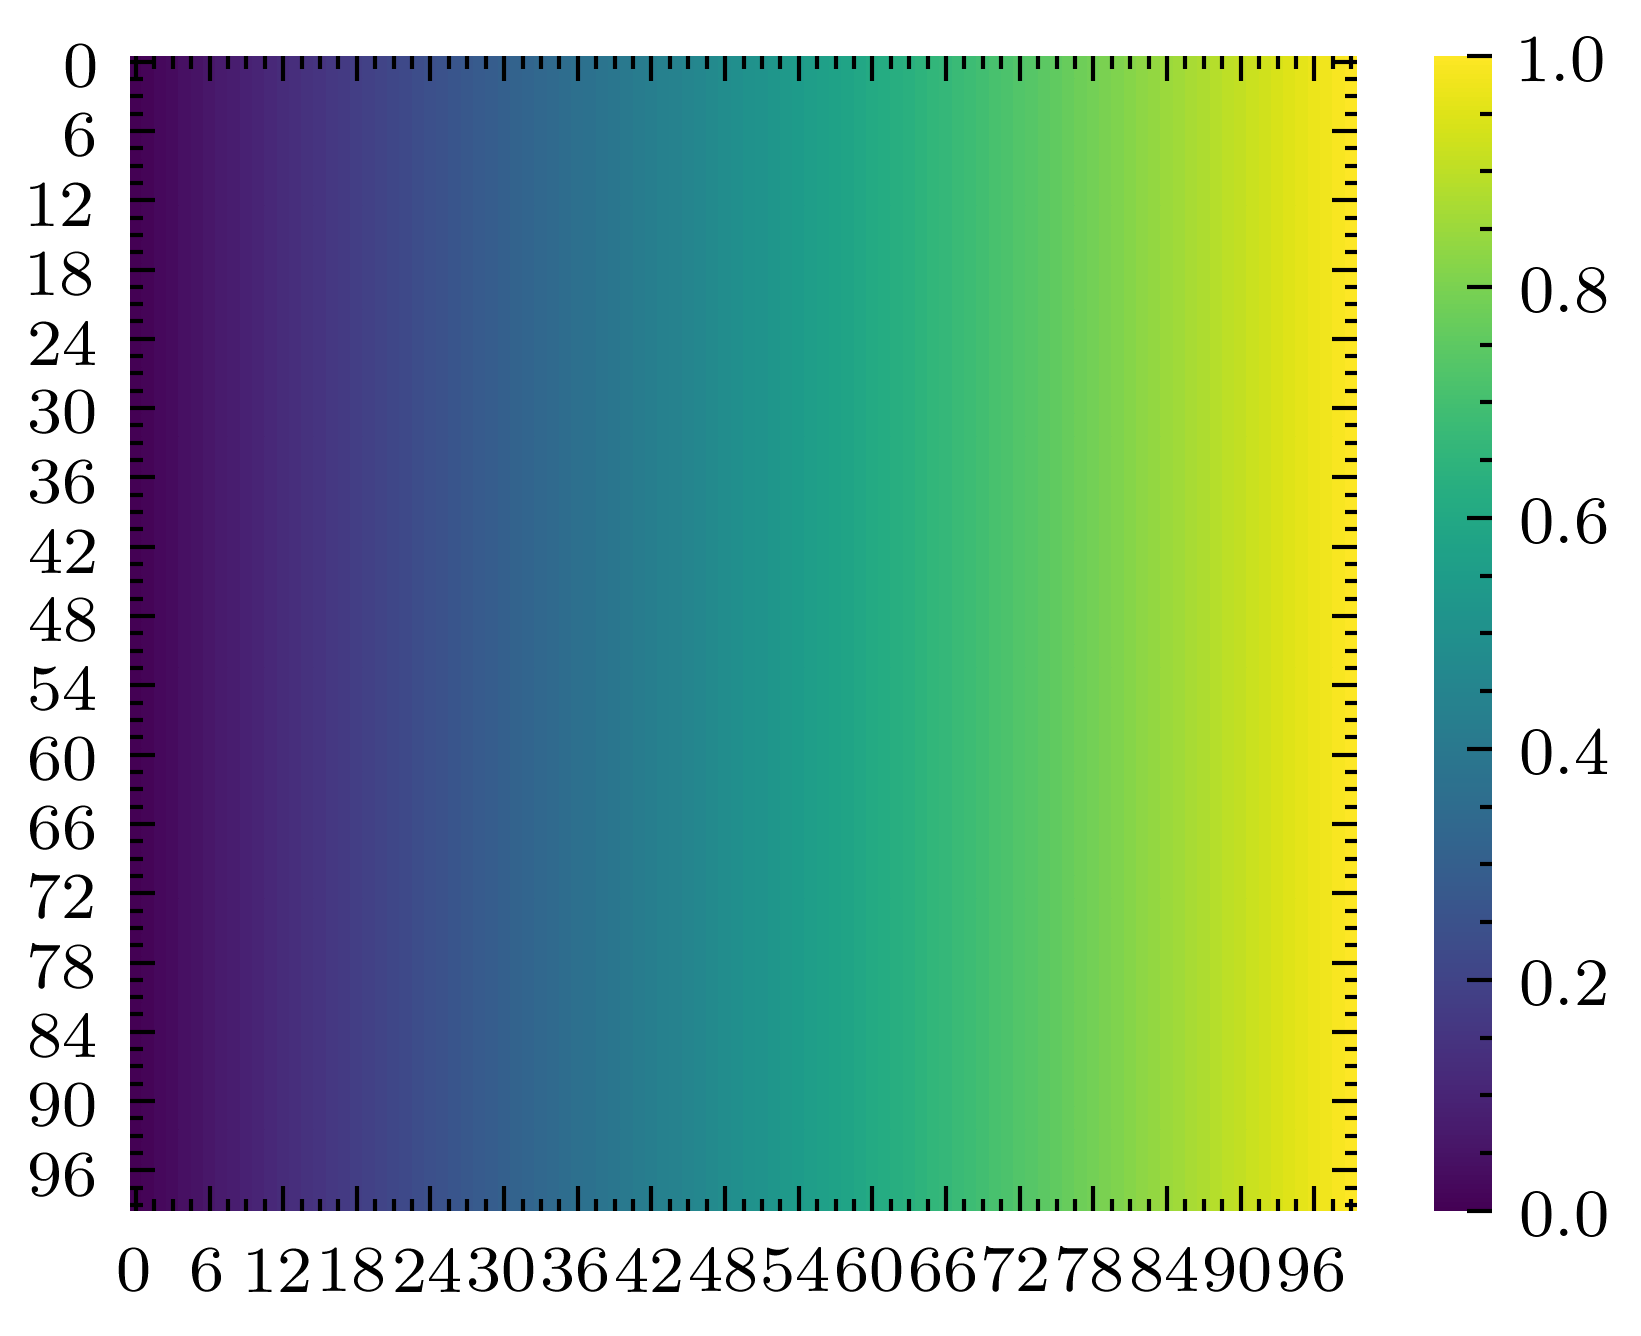
\includegraphics[width=\textwidth]{../img/data-aug/2d/ramp.png}
            \caption{Ramp}
        \end{subfigure}
        \begin{subfigure}[b]{0.45\linewidth}
            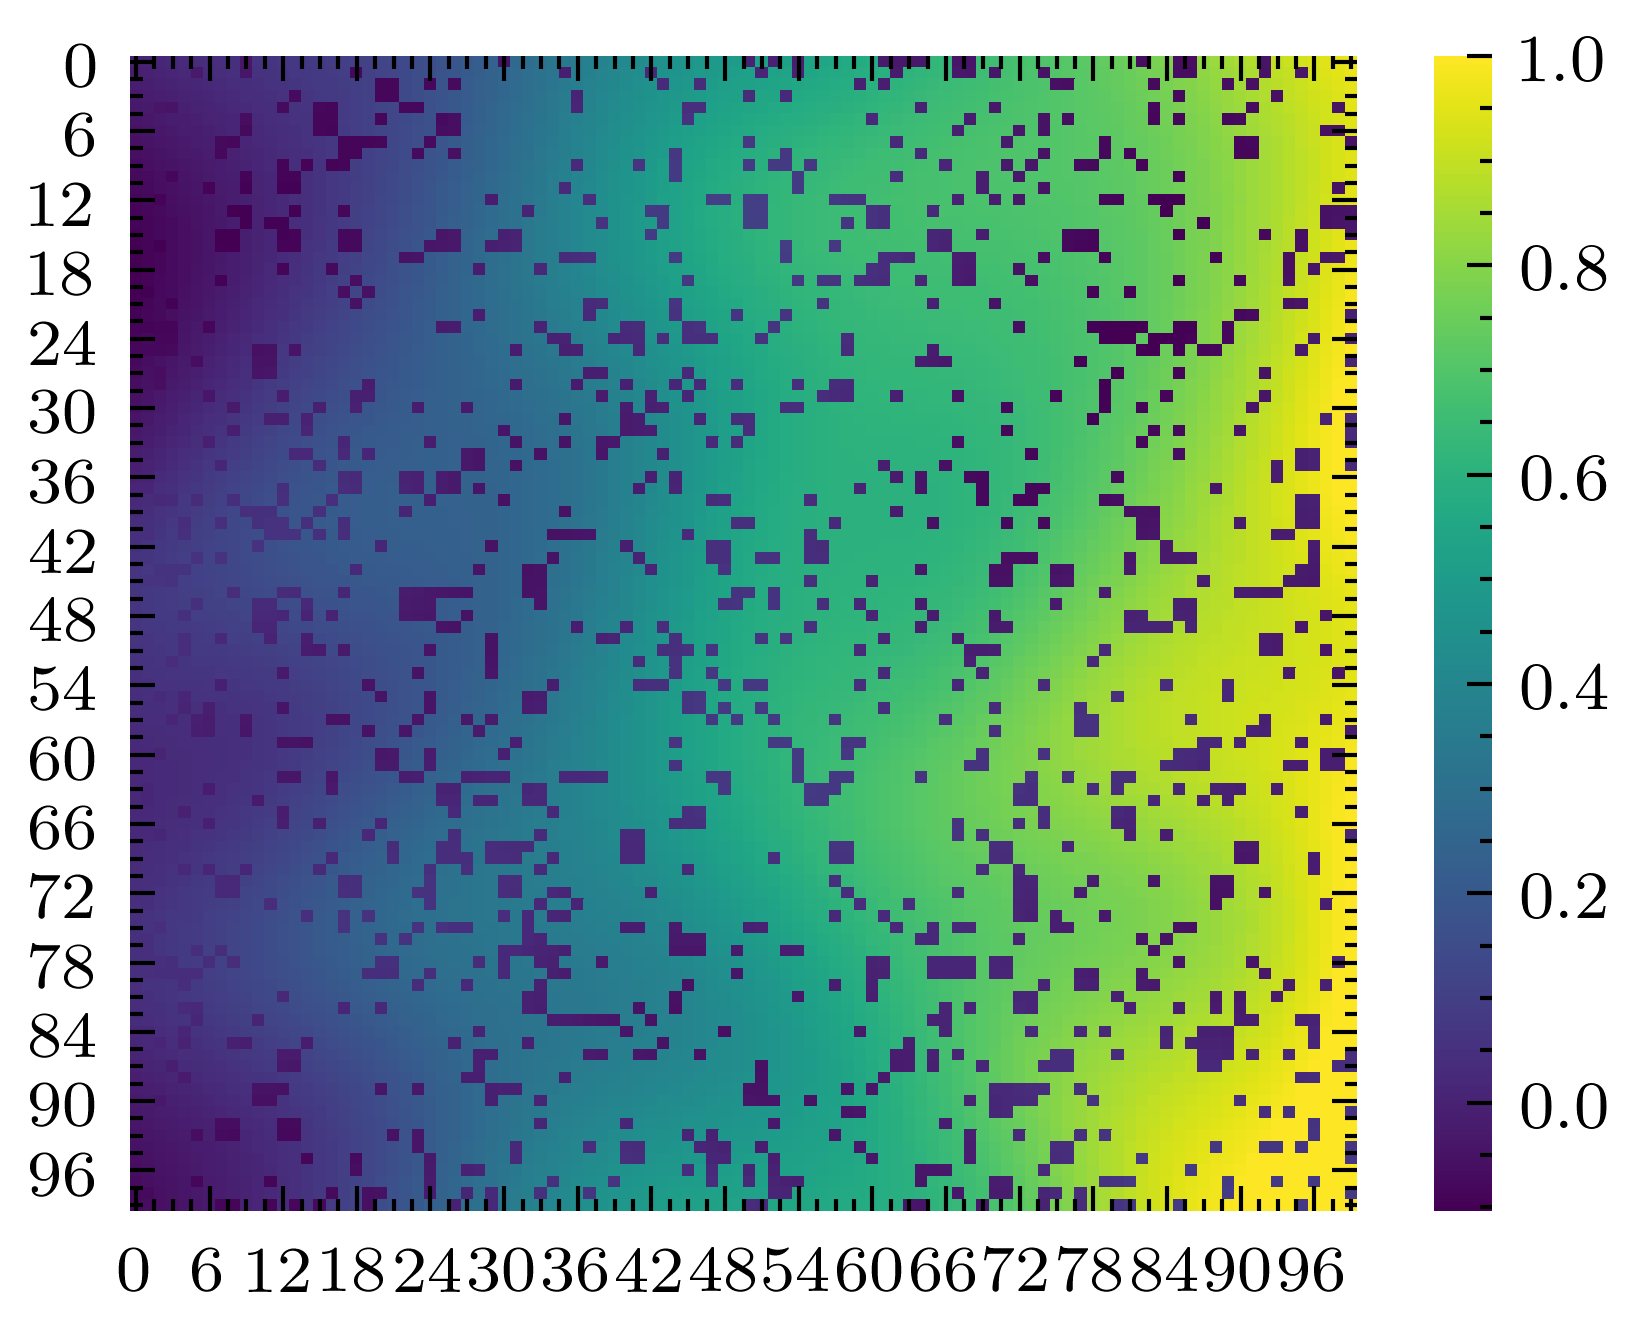
\includegraphics[width=\textwidth]{../img/data-aug/2d/ramp-aug.png}
            \caption{ramp aug}
        \end{subfigure}    
    \label{fig: others-aug}
    \caption{Wall}    
\end{figure}
In all the traning epochs, we apply data-augmentation to each input image $x$ with a probability of $0.8$. Dropout has a probability between $0.05$ and $0.1$. Coarse dropout with a probability of $0.02$ and $0.1$ with a size of the lower resolution image from which to sample the dropout between $0.6$ and $0.8$. Simplex noise with a feature size between $1$ and $50$ with a random scaling factor between $6$ and $10$. 
\end{document}